% Options for packages loaded elsewhere
\PassOptionsToPackage{unicode}{hyperref}
\PassOptionsToPackage{hyphens}{url}
%
\documentclass[
]{book}
\usepackage{lmodern}
\usepackage{amssymb,amsmath}
\usepackage{ifxetex,ifluatex}
\ifnum 0\ifxetex 1\fi\ifluatex 1\fi=0 % if pdftex
  \usepackage[T1]{fontenc}
  \usepackage[utf8]{inputenc}
  \usepackage{textcomp} % provide euro and other symbols
\else % if luatex or xetex
  \usepackage{unicode-math}
  \defaultfontfeatures{Scale=MatchLowercase}
  \defaultfontfeatures[\rmfamily]{Ligatures=TeX,Scale=1}
\fi
% Use upquote if available, for straight quotes in verbatim environments
\IfFileExists{upquote.sty}{\usepackage{upquote}}{}
\IfFileExists{microtype.sty}{% use microtype if available
  \usepackage[]{microtype}
  \UseMicrotypeSet[protrusion]{basicmath} % disable protrusion for tt fonts
}{}
\makeatletter
\@ifundefined{KOMAClassName}{% if non-KOMA class
  \IfFileExists{parskip.sty}{%
    \usepackage{parskip}
  }{% else
    \setlength{\parindent}{0pt}
    \setlength{\parskip}{6pt plus 2pt minus 1pt}}
}{% if KOMA class
  \KOMAoptions{parskip=half}}
\makeatother
\usepackage{xcolor}
\IfFileExists{xurl.sty}{\usepackage{xurl}}{} % add URL line breaks if available
\IfFileExists{bookmark.sty}{\usepackage{bookmark}}{\usepackage{hyperref}}
\hypersetup{
  pdftitle={vignette},
  hidelinks,
  pdfcreator={LaTeX via pandoc}}
\urlstyle{same} % disable monospaced font for URLs
\usepackage{color}
\usepackage{fancyvrb}
\newcommand{\VerbBar}{|}
\newcommand{\VERB}{\Verb[commandchars=\\\{\}]}
\DefineVerbatimEnvironment{Highlighting}{Verbatim}{commandchars=\\\{\}}
% Add ',fontsize=\small' for more characters per line
\usepackage{framed}
\definecolor{shadecolor}{RGB}{248,248,248}
\newenvironment{Shaded}{\begin{snugshade}}{\end{snugshade}}
\newcommand{\AlertTok}[1]{\textcolor[rgb]{0.94,0.16,0.16}{#1}}
\newcommand{\AnnotationTok}[1]{\textcolor[rgb]{0.56,0.35,0.01}{\textbf{\textit{#1}}}}
\newcommand{\AttributeTok}[1]{\textcolor[rgb]{0.77,0.63,0.00}{#1}}
\newcommand{\BaseNTok}[1]{\textcolor[rgb]{0.00,0.00,0.81}{#1}}
\newcommand{\BuiltInTok}[1]{#1}
\newcommand{\CharTok}[1]{\textcolor[rgb]{0.31,0.60,0.02}{#1}}
\newcommand{\CommentTok}[1]{\textcolor[rgb]{0.56,0.35,0.01}{\textit{#1}}}
\newcommand{\CommentVarTok}[1]{\textcolor[rgb]{0.56,0.35,0.01}{\textbf{\textit{#1}}}}
\newcommand{\ConstantTok}[1]{\textcolor[rgb]{0.00,0.00,0.00}{#1}}
\newcommand{\ControlFlowTok}[1]{\textcolor[rgb]{0.13,0.29,0.53}{\textbf{#1}}}
\newcommand{\DataTypeTok}[1]{\textcolor[rgb]{0.13,0.29,0.53}{#1}}
\newcommand{\DecValTok}[1]{\textcolor[rgb]{0.00,0.00,0.81}{#1}}
\newcommand{\DocumentationTok}[1]{\textcolor[rgb]{0.56,0.35,0.01}{\textbf{\textit{#1}}}}
\newcommand{\ErrorTok}[1]{\textcolor[rgb]{0.64,0.00,0.00}{\textbf{#1}}}
\newcommand{\ExtensionTok}[1]{#1}
\newcommand{\FloatTok}[1]{\textcolor[rgb]{0.00,0.00,0.81}{#1}}
\newcommand{\FunctionTok}[1]{\textcolor[rgb]{0.00,0.00,0.00}{#1}}
\newcommand{\ImportTok}[1]{#1}
\newcommand{\InformationTok}[1]{\textcolor[rgb]{0.56,0.35,0.01}{\textbf{\textit{#1}}}}
\newcommand{\KeywordTok}[1]{\textcolor[rgb]{0.13,0.29,0.53}{\textbf{#1}}}
\newcommand{\NormalTok}[1]{#1}
\newcommand{\OperatorTok}[1]{\textcolor[rgb]{0.81,0.36,0.00}{\textbf{#1}}}
\newcommand{\OtherTok}[1]{\textcolor[rgb]{0.56,0.35,0.01}{#1}}
\newcommand{\PreprocessorTok}[1]{\textcolor[rgb]{0.56,0.35,0.01}{\textit{#1}}}
\newcommand{\RegionMarkerTok}[1]{#1}
\newcommand{\SpecialCharTok}[1]{\textcolor[rgb]{0.00,0.00,0.00}{#1}}
\newcommand{\SpecialStringTok}[1]{\textcolor[rgb]{0.31,0.60,0.02}{#1}}
\newcommand{\StringTok}[1]{\textcolor[rgb]{0.31,0.60,0.02}{#1}}
\newcommand{\VariableTok}[1]{\textcolor[rgb]{0.00,0.00,0.00}{#1}}
\newcommand{\VerbatimStringTok}[1]{\textcolor[rgb]{0.31,0.60,0.02}{#1}}
\newcommand{\WarningTok}[1]{\textcolor[rgb]{0.56,0.35,0.01}{\textbf{\textit{#1}}}}
\usepackage{longtable,booktabs}
% Correct order of tables after \paragraph or \subparagraph
\usepackage{etoolbox}
\makeatletter
\patchcmd\longtable{\par}{\if@noskipsec\mbox{}\fi\par}{}{}
\makeatother
% Allow footnotes in longtable head/foot
\IfFileExists{footnotehyper.sty}{\usepackage{footnotehyper}}{\usepackage{footnote}}
\makesavenoteenv{longtable}
\usepackage{graphicx,grffile}
\makeatletter
\def\maxwidth{\ifdim\Gin@nat@width>\linewidth\linewidth\else\Gin@nat@width\fi}
\def\maxheight{\ifdim\Gin@nat@height>\textheight\textheight\else\Gin@nat@height\fi}
\makeatother
% Scale images if necessary, so that they will not overflow the page
% margins by default, and it is still possible to overwrite the defaults
% using explicit options in \includegraphics[width, height, ...]{}
\setkeys{Gin}{width=\maxwidth,height=\maxheight,keepaspectratio}
% Set default figure placement to htbp
\makeatletter
\def\fps@figure{htbp}
\makeatother
\setlength{\emergencystretch}{3em} % prevent overfull lines
\providecommand{\tightlist}{%
  \setlength{\itemsep}{0pt}\setlength{\parskip}{0pt}}
\setcounter{secnumdepth}{5}
\usepackage{booktabs}
\usepackage{amsthm}
\usepackage[left=2cm,right=2cm,top=2cm,bottom=2cm]{geometry}
\makeatletter
\def\thm@space@setup{%
  \thm@preskip=8pt plus 2pt minus 4pt
  \thm@postskip=\thm@preskip
}
\makeatother
\usepackage[]{natbib}
\bibliographystyle{apalike}

\title{vignette}
\author{}
\date{\vspace{-2.5em}}

\begin{document}
\maketitle

{
\setcounter{tocdepth}{1}
\tableofcontents
}
\hypertarget{status}{%
\chapter{Status}\label{status}}

This status report outlines the code we are developing to process \texttt{WinCruz} data and prepare it for density estimation analysis using \texttt{distance} and related packages in \texttt{R}.

\hypertarget{changes}{%
\subsubsection*{Changes}\label{changes}}
\addcontentsline{toc}{subsubsection}{Changes}

\begin{itemize}
\item
  New \textbf{status report format} (a \texttt{bookdown} vignette, compatible with a future website and PDF tutorial.)
\item
  \textbf{Initiation of package framework} (more efficient to design, develop, test, and document code). See \texttt{Install} chapter for details.
\item
  Implementation of \textbf{new settings system}: survey-wide and cohort-specific settings. See \texttt{Settings} chapter for description / explanation.
\item
  Update of strata and segmentizing functions to accommodate new settings system. See \texttt{Processing} chapter.
\item
  The function \texttt{process\_polygon()} now calculates the area, in km2, of strata and study area polygons.
\end{itemize}

\hypertarget{next-focus}{%
\subsubsection*{Next focus}\label{next-focus}}
\addcontentsline{toc}{subsubsection}{Next focus}

\begin{itemize}
\tightlist
\item
  Transfer code to the new settings system and package framework:
\end{itemize}

--- mapping functions\\
--- sightings processing\\
--- survey summary

\begin{itemize}
\item
  Update backlog
\item
  Back to developing the sightings processing
\end{itemize}

\hypertarget{questions-for-amanda}{%
\subsubsection*{Questions for Amanda}\label{questions-for-amanda}}
\addcontentsline{toc}{subsubsection}{Questions for Amanda}

\begin{itemize}
\item
  Lots of structural changes (new vignette system, initiation of package framework). Lots on my list to do to complete the transfer, so not many questions for now.
\item
  Am I getting closer with the new settings / segmentizing frameworks?
\end{itemize}

\hypertarget{install}{%
\chapter{\texorpdfstring{Install \texttt{LTabundR}}{Install LTabundR}}\label{install}}

\hypertarget{option-1-install-from-github}{%
\section*{Option 1: Install from GitHub}\label{option-1-install-from-github}}
\addcontentsline{toc}{section}{Option 1: Install from GitHub}

Since the package is currently private, this is more complicated than it will be once the package is released.

The first step is creating an \texttt{R} environment variable containing your \texttt{GitHub} personal access token.

Complete these instructions \textbf{only once:}

\begin{Shaded}
\begin{Highlighting}[]
\CommentTok{# Open your .Renviron file}
\KeywordTok{library}\NormalTok{(usethis)}
\NormalTok{usethis}\OperatorTok{::}\KeywordTok{edit_r_environ}\NormalTok{()}

\CommentTok{# Add your GitHub personal access token as a variable in `.Renviron`}
\NormalTok{GITHUB_TOKEN <-}\StringTok{ 'your_token_goes_here_as_a_character_string'}

\CommentTok{# Save and close your .Renviron file}
\CommentTok{# Reload .Renviron}
\KeywordTok{readRenviron}\NormalTok{(}\StringTok{'~/.Renviron'}\NormalTok{)}
\end{Highlighting}
\end{Shaded}

Then run this code \textbf{every time} you want to reinstall / update the package:

\begin{Shaded}
\begin{Highlighting}[]
\KeywordTok{library}\NormalTok{(devtools)}
\NormalTok{github_token <-}\StringTok{ }\KeywordTok{Sys.getenv}\NormalTok{(}\StringTok{"GITHUB_TOKEN"}\NormalTok{)}
\NormalTok{devtools}\OperatorTok{::}\KeywordTok{install_github}\NormalTok{(}\DataTypeTok{repo =} \StringTok{'amandalbradford/LTabundR-dev'}\NormalTok{,}
                         \DataTypeTok{subdir=}\StringTok{'LTabundR'}\NormalTok{,}
                         \DataTypeTok{auth_token=}\NormalTok{github_token)}
\KeywordTok{library}\NormalTok{(LTabundR)}
\end{Highlighting}
\end{Shaded}

\hypertarget{option-2-install-locally}{%
\section*{Option 2: Install locally}\label{option-2-install-locally}}
\addcontentsline{toc}{section}{Option 2: Install locally}

For now you can also install or update the package locally, using this code:

\begin{Shaded}
\begin{Highlighting}[]
\KeywordTok{library}\NormalTok{(devtools) }

\CommentTok{# Remove the package, if you have an earlier version of it on your machine}
\ControlFlowTok{if}\NormalTok{(}\StringTok{'LTAabundR'} \OperatorTok\StringTok{ }\KeywordTok{installed.packages}\NormalTok{())\{}\KeywordTok{remove.packages}\NormalTok{(}\StringTok{'LTabundR'}\NormalTok{)\} }

\CommentTok{# Specify the path to the package's project folder.}
\NormalTok{path_to_package <-}\StringTok{ '../LTabundR'}

\CommentTok{# Update function documentation}
\KeywordTok{document}\NormalTok{(path_to_package) }

\CommentTok{# Install package and any dependencies you need}
\KeywordTok{install}\NormalTok{(path_to_package) }

\KeywordTok{library}\NormalTok{(LTabundR)}
\end{Highlighting}
\end{Shaded}

\hypertarget{settings}{%
\chapter{Settings}\label{settings}}

To customize the way data are processed and included in your analysis, use the \texttt{load\_settings()} function. This function emulates and expands upon the settings file, \texttt{ABUND.INP}, that was used to run \texttt{ABUND7/9} in \texttt{FORTRAN}.

This function allows you to use `factory defaults' if you don't wish to specify anything special such as strata or study area polygons:

\begin{Shaded}
\begin{Highlighting}[]
\NormalTok{settings <-}\StringTok{ }\KeywordTok{load_settings}\NormalTok{()}
\end{Highlighting}
\end{Shaded}

If you do not want to use all the defaults, you can give \texttt{load\_settings()} some custom inputs. The function accepts four arguments:

\begin{itemize}
\item
  \texttt{strata}: dataframe(s) of coordinates
\item
  \texttt{study\_area}: a dataframe of coordinates
\item
  \texttt{survey}: settings that will apply universally to the analysis
\item
  \texttt{cohorts}: settings that are specific to groups of species. By providing cohort-specific settings, the code for a single analysis becomes fully flexible to prepare and more easily reproduced, since code need not be modified in order to replicate the analysis in full.
\end{itemize}

The output of \texttt{load\_settings()} is a named list with a slot for each of these arguments:

\begin{Shaded}
\begin{Highlighting}[]
\NormalTok{settings }\OperatorTok\StringTok{ }\NormalTok{names}
\NormalTok{[}\DecValTok{1}\NormalTok{] }\StringTok{"strata"}     \StringTok{"study_area"} \StringTok{"survey"}     \StringTok{"cohorts"}   
\end{Highlighting}
\end{Shaded}

\hypertarget{survey-strata}{%
\section*{Survey strata}\label{survey-strata}}
\addcontentsline{toc}{section}{Survey strata}

Stratum polygons can be provided as a named list of \texttt{data.frame} objects. Each \texttt{data.frame} must have \texttt{Lat} and \texttt{Lon} as the first two columns, providing coordinates in decimal degrees in which South and West coordinates are negative. Other columns are allowed, but the first two need to be \texttt{Lon} and \texttt{Lat}. The name of the slot holding the \texttt{data.frame} will be used as a reference name for the stratum.

If \texttt{strata} is \texttt{NULL}, abundance will not be estimated; only density within the searched area (i.e., the total segment length x effective strip width).

While users are welcome to upload polygons of their own, the package comes with ``stock'' polygons for strata that are commonly used in the main NMFS study regions: the Central North Pacific (CNP, including Hawaii) \ldots{}

\begin{Shaded}
\begin{Highlighting}[]
\KeywordTok{data}\NormalTok{(strata_cnp) }
\KeywordTok{names}\NormalTok{(strata_cnp)}
\NormalTok{[}\DecValTok{1}\NormalTok{] }\StringTok{"HI_EEZ"}   \StringTok{"WHICEAS"}  \StringTok{"OtherCNP"}
\end{Highlighting}
\end{Shaded}

\ldots the California Current System (CCS) \ldots{}

\begin{Shaded}
\begin{Highlighting}[]
\KeywordTok{data}\NormalTok{(strata_ccs) }
\KeywordTok{names}\NormalTok{(strata_ccs)}
\NormalTok{[}\DecValTok{1}\NormalTok{] }\StringTok{"CCS"}         \StringTok{"Southern_CA"} \StringTok{"Central_CA"}  \StringTok{"Nothern_CA"}  \StringTok{"OR_WA"}      
\end{Highlighting}
\end{Shaded}

\ldots{} and the Eastern Tropical Pacific (ETP):

\begin{Shaded}
\begin{Highlighting}[]
\KeywordTok{data}\NormalTok{(strata_etp) }
\KeywordTok{names}\NormalTok{(strata_etp)}
\NormalTok{ [}\DecValTok{1}\NormalTok{] }\StringTok{"MOPS_AreaCoreM"}     \StringTok{"MOPS_AreaIn"}        \StringTok{"MOPS_AreaIn1"}      
\NormalTok{ [}\DecValTok{4}\NormalTok{] }\StringTok{"MOPS_AreaIn2"}       \StringTok{"MOPS_AREAINS"}       \StringTok{"MOPS_AREAMID"}      
\NormalTok{ [}\DecValTok{7}\NormalTok{] }\StringTok{"MOPS_AreaMid1"}      \StringTok{"MOPS_AreaMid2"}      \StringTok{"MOPS_AreaMOPS"}     
\NormalTok{[}\DecValTok{10}\NormalTok{] }\StringTok{"MOPS_AREANORS"}      \StringTok{"MOPS_AreaOuterM"}    \StringTok{"MOPS_AreaSou"}      
\NormalTok{[}\DecValTok{13}\NormalTok{] }\StringTok{"MOPS_AREASOUS"}      \StringTok{"MOPS_AreaSpin"}      \StringTok{"MOPS_AreaSpinS"}    
\NormalTok{[}\DecValTok{16}\NormalTok{] }\StringTok{"MOPS_AREAWES"}       \StringTok{"PODS_93STRAT1"}      \StringTok{"PODS_93STRAT2"}     
\NormalTok{[}\DecValTok{19}\NormalTok{] }\StringTok{"PODS_Area92"}        \StringTok{"PODS_AREA92RS"}      \StringTok{"PODS_Area92s"}      
\NormalTok{[}\DecValTok{22}\NormalTok{] }\StringTok{"PODS_AREA93"}        \StringTok{"PODS_AREA93A"}       \StringTok{"PODS_AREA93AR"}     
\NormalTok{[}\DecValTok{25}\NormalTok{] }\StringTok{"PODS_AREA93AS"}      \StringTok{"PODS_AREA93BR"}      \StringTok{"PODS_AREA93M"}      
\NormalTok{[}\DecValTok{28}\NormalTok{] }\StringTok{"PODS_AREA93MS"}      \StringTok{"PODS_AREA93R"}       \StringTok{"PODS_AREA93R1"}     
\NormalTok{[}\DecValTok{31}\NormalTok{] }\StringTok{"PODS_AREA93R2"}      \StringTok{"PODS_AREA93RS"}      \StringTok{"PODS_AREA93S"}      
\NormalTok{[}\DecValTok{34}\NormalTok{] }\StringTok{"PODS_AREANCOR"}      \StringTok{"PODS_GOCpoly"}       \StringTok{"Pre1986_Area79ES1"} 
\NormalTok{[}\DecValTok{37}\NormalTok{] }\StringTok{"Pre1986_Area79ES1s"} \StringTok{"Pre1986_Area79ES2"}  \StringTok{"Pre1986_Area79ES2s"}
\NormalTok{[}\DecValTok{40}\NormalTok{] }\StringTok{"Pre1986_Area79NE1"}  \StringTok{"Pre1986_Area79NE1s"} \StringTok{"Pre1986_Area79NE2"} 
\NormalTok{[}\DecValTok{43}\NormalTok{] }\StringTok{"Pre1986_Area79NE2s"} \StringTok{"Pre1986_Area79NE3"}  \StringTok{"Pre1986_Area79NE3s"}
\NormalTok{[}\DecValTok{46}\NormalTok{] }\StringTok{"Pre1986_AreaCal"}    \StringTok{"Pre1986_AreaCals"}   \StringTok{"Pre1986_AreaMid"}   
\NormalTok{[}\DecValTok{49}\NormalTok{] }\StringTok{"Pre1986_AreaMidS"}   \StringTok{"Pre1986_AreaNorth"}  \StringTok{"Pre1986_AreaNorthS"}
\NormalTok{[}\DecValTok{52}\NormalTok{] }\StringTok{"Pre1986_AreaSouth"}  \StringTok{"Pre1986_AreaSouthS"} \StringTok{"STAR_Area98a"}      
\NormalTok{[}\DecValTok{55}\NormalTok{] }\StringTok{"STAR_Area98b"}       \StringTok{"STAR_AreaCore"}      \StringTok{"STAR_AreaCore2"}    
\NormalTok{[}\DecValTok{58}\NormalTok{] }\StringTok{"STAR_AreaCoreS"}     \StringTok{"STAR_AreaNCoast"}    \StringTok{"STAR_AreaNCstS"}    
\NormalTok{[}\DecValTok{61}\NormalTok{] }\StringTok{"STAR_AreaOuter"}     \StringTok{"STAR_AreaOuter00"}   \StringTok{"STAR_AreaSCoast"}   
\NormalTok{[}\DecValTok{64}\NormalTok{] }\StringTok{"STAR_AreaSCstS"}     \StringTok{"STAR_AreaSPn"}       \StringTok{"STAR_AreaSPs"}      
\NormalTok{[}\DecValTok{67}\NormalTok{] }\StringTok{"STAR_AreaSTAR"}      \StringTok{"STAR_AreaSTAR2"}     \StringTok{"STAR_AreaSTARlite"} 
\NormalTok{[}\DecValTok{70}\NormalTok{] }\StringTok{"STAR_Dcaparea"}     
\end{Highlighting}
\end{Shaded}

The package includes functions for visualizing and selecting from these strata. See the \protect\hyperlink{stratagallery}{Strata Gallery} appendix.

\hypertarget{study-area-polygon}{%
\section*{Study area polygon}\label{study-area-polygon}}
\addcontentsline{toc}{section}{Study area polygon}

The \texttt{study\_area} argument accepts a single \texttt{data.frame}, formatted the same as those for the \texttt{strata} argument, or a numeric value indicating the area of your study area in square km. If \texttt{study\_area} is \texttt{NULL}, abundance will not be estimated; only density.

Study area polygons can be provided in the same format as strata: a two-column \texttt{csv} (column names \texttt{Lon} and \texttt{Lat} with decimal-degree coordinates).

A stock study area polygon is available for the CNP:

\begin{Shaded}
\begin{Highlighting}[]
\KeywordTok{data}\NormalTok{(study_cnp) }
\NormalTok{study_cnp}
\NormalTok{   Lon   Lat}
\DecValTok{1} \DecValTok{-131} \FloatTok{40.00}
\DecValTok{2} \DecValTok{-126} \FloatTok{32.05}
\DecValTok{3} \DecValTok{-120} \FloatTok{25.00}
\DecValTok{4} \DecValTok{-120} \FloatTok{-5.00}
\DecValTok{5} \DecValTok{-185} \FloatTok{-5.00}
\DecValTok{6} \DecValTok{-185} \FloatTok{40.00}
\DecValTok{7} \DecValTok{-131} \FloatTok{40.00}
\end{Highlighting}
\end{Shaded}

\hypertarget{survey-wide-settings}{%
\section*{Survey-wide settings}\label{survey-wide-settings}}
\addcontentsline{toc}{section}{Survey-wide settings}

Survey-wide settings apply universally to all species in the analysis.

\hypertarget{defaults}{%
\subsection*{Defaults}\label{defaults}}
\addcontentsline{toc}{subsection}{Defaults}

\begin{Shaded}
\begin{Highlighting}[]
\NormalTok{settings}\OperatorTok{$}\NormalTok{survey}
\OperatorTok{$}\NormalTok{segment_method}
\NormalTok{[}\DecValTok{1}\NormalTok{] }\StringTok{"day"}

\OperatorTok{$}\NormalTok{segment_target_km}
\NormalTok{[}\DecValTok{1}\NormalTok{] }\DecValTok{150}

\OperatorTok{$}\NormalTok{segment_max_km_gap}
\NormalTok{[}\DecValTok{1}\NormalTok{] }\DecValTok{5}

\OperatorTok{$}\NormalTok{segment_max_interval}
\NormalTok{[}\DecValTok{1}\NormalTok{] }\DecValTok{48}

\OperatorTok{$}\NormalTok{segment_type_handling}
\NormalTok{[}\DecValTok{1}\NormalTok{] }\StringTok{"separate"} \StringTok{"pool"}    

\OperatorTok{$}\NormalTok{segment_remainder_handling}
\NormalTok{[}\DecValTok{1}\NormalTok{] }\StringTok{"append"}  \StringTok{"segment"}

\OperatorTok{$}\NormalTok{ship_list}
\OtherTok{NULL}

\OperatorTok{$}\NormalTok{species_codes}
\OtherTok{NULL}

\OperatorTok{$}\NormalTok{group_size_coefficients}
\OtherTok{NULL}

\OperatorTok{$}\NormalTok{smear_angles}
\NormalTok{[}\DecValTok{1}\NormalTok{] }\OtherTok{FALSE}

\OperatorTok{$}\NormalTok{random_seed}
\NormalTok{[}\DecValTok{1}\NormalTok{] }\DecValTok{833171}

\OperatorTok{$}\NormalTok{verbose}
\NormalTok{[}\DecValTok{1}\NormalTok{] }\OtherTok{TRUE}
\end{Highlighting}
\end{Shaded}

Defaults for the \texttt{survey} argument list are built up efficiently using the function \texttt{load\_survey\_settings()} (see example code at bottom).

\hypertarget{details}{%
\subsection*{Details}\label{details}}
\addcontentsline{toc}{subsection}{Details}

The \texttt{survey\_settings} input accepts a list with any of the following named slots:

\begin{itemize}
\item
  \textbf{\texttt{segment\_method:}} this argument controls how effort will be ``segmentized'', or chopped into discrete sections for the purposes of estimating the variance of the abundance estimate. The two options are \texttt{"day"} -- all effort within the same Cruise-StudyArea-Stratum-Year-Effort will be binned into segments by calendar date -- and \texttt{"equallength"} -- effort within each unique effort scenario (Cruise-StudyArea-etc.) will be divided into segments of approximately equal length.
\item
  \textbf{\texttt{segment\_target\_km:}} if segmenting by \texttt{"equallength"}, this field allows you to specify what that target length is, in km.
\item
  \textbf{\texttt{segment\_max\_km\_gap:}} the segmentizing function works by calculating the distance between each row of \texttt{DAS} data. If that distance exceeds the length specified here (e.g., 5 km), the function will assume that there was a break in effort.
\item
  \textbf{\texttt{segment\_max\_interval:}} if segmentizing by \texttt{"equallength"}, this setting allows you to specify the time gaps in effort contained within a single segment. For example, if your goal is a few large segments of equal length (e.g., 150-km segments, for bootstrap estimation of density variance), you are probably willing for discrete periods of effort to be concatenated into a single segment, even if the gaps between effort are as large as 1 or 2 days, in which case you would set \texttt{segment\_max\_interval} to 24 or 48 (hours), respectively. However, if your goal is many smaller segments (e.g., 5-km segments, for habitat modeling), you want to ensure that effort is contiguous so that segment locations can be accurately related to environmental variables, in which case you would set \texttt{segment\_max\_interval} to be very small (e.g., .1 or 6 minutes).
\item
  \textbf{\texttt{segment\_type\_handling:}} if \texttt{"pool"}, all effort types that qualify as valid according to \texttt{cohort\_settings} (see next section) will be pooled together, making it possible for different effort types to occur in the same segment (e.g., \texttt{EffType}'s ``\texttt{S}'' and ``\texttt{F}'' are allowed to occur in the same segment; if this argument is \texttt{"separate"}, segments will only be allowed to contain a single effort type.
\item
  \textbf{\texttt{segment\_remainder\_handling:}} if segmentizing by \texttt{"equallength"}, periods of contiguous effort (as specified by \texttt{segment\_max\_interval}) are unlikely to be perfectly divisible by your \texttt{segment\_target\_km}; there is going to be a remainder. You can handle this remainder in various ways: (1) \texttt{"disperse"} allows the function to adjust \texttt{segment\_target\_km} so that there is in fact no remainder, effectively dispersing the remainder evenly across all segments within that period of contiguous effort; (2) \texttt{"append"} asks the function to append the remainder to a randomly selected segment; (3) \texttt{"segment"} asks the function to simply place the remainder in its own segment, placed randomly within the period of contiguous effort. Note that this setting has a second layer of versatility, because it can accept a one- or two-element character vector. If a two-element vector is provided (e.g., \texttt{c("append","segment")}), the first element will be used in the event that the remainder is less than or equal to half \texttt{segment\_target\_km}; if the remainder is more than half that target length, the second element will be used. This feature allows for replication of the segmentizing methods in \href{https://www.int-res.com/abstracts/meps/v413/p163-183/}{Becker et al.~(2010)}.
\item
  \textbf{\texttt{ship\_list:}} A \texttt{data.frame} containing a list of ship names. If not provided the default version, which was current as of the release of \texttt{ABUND9} in 2020, will be used (\texttt{data(ships)}). Supplied \texttt{data.frames} must match the column naming structure of \texttt{data(ships)}. (\emph{Note: the purpose of this argument in the \texttt{INP} file is not clear to me; need to understand how/why to include this. -- eric})
\item
  \textbf{\texttt{species\_codes:}} A \texttt{data.frame} containing species codes. If not provided the default version, which was current as of the release of \texttt{ABUND9} in 2020, will be used (\texttt{data(species\_codes)}). Supplied \texttt{data.frames} must match the column naming structure of \texttt{data(species\_codes)}.
\item
  \textbf{\texttt{group\_size\_coefficients:}} A \texttt{data.frame} of calibration factors. \emph{NOTE: details needed here.}
\item
  \textbf{\texttt{smear\_angles:}} If \texttt{TRUE} (the default is \texttt{FALSE}), bearing angles to a group of animals will be ``smeared'' by adding a uniformly distributed random number between -5 and +5 degrees. This has not been used in any recent analyses because observers have not been rounding angles as much. It was suggested by Buckland as a method for dealing with rounding which is especially influential when rounding to zero places many sightings at zero perpendicular distance.
\item
  \textbf{\texttt{random\_seed:}} a number used as the seed for stages involving random number generation. If not \texttt{NULL}, the results will be exactly reproducible. Default is \texttt{833171} (\emph{sensu} example code in \texttt{ABUND9}).
\item
  \textbf{\texttt{verbose:}} If \texttt{TRUE} (the default), status updates will be printed to the \texttt{R} console.
\end{itemize}

\hypertarget{cohort-specific-settings}{%
\section*{Cohort-specific settings}\label{cohort-specific-settings}}
\addcontentsline{toc}{section}{Cohort-specific settings}

Cohort-specific settings apply only to a group of species.

\hypertarget{defaults-1}{%
\subsection*{Defaults}\label{defaults-1}}
\addcontentsline{toc}{subsection}{Defaults}

The default is to use a single cohort for all species:

\begin{Shaded}
\begin{Highlighting}[]
\NormalTok{settings}\OperatorTok{$}\NormalTok{cohorts }\OperatorTok\StringTok{ }\NormalTok{names}
\NormalTok{[}\DecValTok{1}\NormalTok{] }\StringTok{"default"}
\end{Highlighting}
\end{Shaded}

Default values for the \texttt{default} cohort:

\begin{Shaded}
\begin{Highlighting}[]
\NormalTok{settings}\OperatorTok{$}\NormalTok{cohorts}\OperatorTok{$}\NormalTok{default}
\OperatorTok{$}\NormalTok{id}
\NormalTok{[}\DecValTok{1}\NormalTok{] }\StringTok{"default"}

\OperatorTok{$}\NormalTok{species}
\OtherTok{NULL}

\OperatorTok{$}\NormalTok{probable_species}
\NormalTok{[}\DecValTok{1}\NormalTok{] }\OtherTok{FALSE}

\OperatorTok{$}\NormalTok{sighting_method}
\NormalTok{[}\DecValTok{1}\NormalTok{] }\DecValTok{0}

\OperatorTok{$}\NormalTok{cue_range}
\NormalTok{[}\DecValTok{1}\NormalTok{] }\DecValTok{0} \DecValTok{1} \DecValTok{2} \DecValTok{3} \DecValTok{4} \DecValTok{5} \DecValTok{6} \DecValTok{7}

\OperatorTok{$}\NormalTok{school_size_range}
\NormalTok{[}\DecValTok{1}\NormalTok{]     }\DecValTok{0} \DecValTok{10000}

\OperatorTok{$}\NormalTok{use_low_if_na}
\NormalTok{[}\DecValTok{1}\NormalTok{] }\OtherTok{FALSE}

\OperatorTok{$}\NormalTok{io_sightings}
\NormalTok{[}\DecValTok{1}\NormalTok{] }\DecValTok{0}

\OperatorTok{$}\NormalTok{geometric_mean_group}
\NormalTok{[}\DecValTok{1}\NormalTok{] }\OtherTok{TRUE}

\OperatorTok{$}\NormalTok{truncation_km}
\NormalTok{[}\DecValTok{1}\NormalTok{] }\FloatTok{5.5}

\OperatorTok{$}\NormalTok{beaufort_range}
\NormalTok{[}\DecValTok{1}\NormalTok{] }\DecValTok{0} \DecValTok{1} \DecValTok{2} \DecValTok{3} \DecValTok{4} \DecValTok{5} \DecValTok{6}

\OperatorTok{$}\NormalTok{abeam_sightings}
\NormalTok{[}\DecValTok{1}\NormalTok{] }\OtherTok{FALSE}

\OperatorTok{$}\NormalTok{strata_overlap_handling}
\NormalTok{[}\DecValTok{1}\NormalTok{] }\StringTok{"smallest"} \StringTok{"largest"}  \StringTok{"each"}    

\OperatorTok{$}\NormalTok{density_types}
\NormalTok{[}\DecValTok{1}\NormalTok{] }\StringTok{"S"} \StringTok{"F"}

\OperatorTok{$}\NormalTok{density_modes}
\NormalTok{[}\DecValTok{1}\NormalTok{] }\StringTok{"P"} \StringTok{"C"}

\OperatorTok{$}\NormalTok{density_on_off}
\NormalTok{[}\DecValTok{1}\NormalTok{] }\OtherTok{TRUE}

\OperatorTok{$}\NormalTok{distance_types}
\OtherTok{NULL}

\OperatorTok{$}\NormalTok{distance_modes}
\OtherTok{NULL}

\OperatorTok{$}\NormalTok{distance_on_off}
\NormalTok{[}\DecValTok{1}\NormalTok{] }\OtherTok{TRUE}
\end{Highlighting}
\end{Shaded}

Defaults for the \texttt{cohorts} argument list is built up efficiently using the function \texttt{load\_cohort\_settings()} (see example code at bottom).

\hypertarget{details-1}{%
\subsection*{Details}\label{details-1}}
\addcontentsline{toc}{subsection}{Details}

The \texttt{cohort\_settings} input accepts a list of any length. Each slot in that list can contain settings for a different cohort. Each cohort list can have any of the following named slots:

\begin{itemize}
\item
  \textbf{\texttt{id:}} An informal identifier for this cohort, to help you keep track of which cohort is which. For example, settings for a cohort of large whales species could be named \texttt{"big\ whales"}; settings for small delphinids and phocoenids could be named \texttt{"small\_odontocetes"}; settings for beaked whales could be named \texttt{"beakers"}.
\item
  \textbf{\texttt{species:}} A vector of species codes to include in this cohort. If \texttt{NULL} (the default), all species will be included.
\item
  \textbf{\texttt{probable\_species:}} If \texttt{TRUE} (default is \texttt{FALSE}), the ``probable'' species identifications will be used in place of the ``unidentified'' categories. The probable species codes are marked with an event code ``?'' in the data file following the ``S'' and ``A'' event codes of a sighting.
\item
  \textbf{\texttt{sighting\_method:}} A coded integer which determines which sightings will be included based on how they were first seen. Allowable codes are 0=any method, 1=with 25X only, 2=not with 25X binos and not from helo (ie. naked eyes and 7x).
\item
  \textbf{\texttt{cue\_range:}} Numeric vector of acceptable ``observation cues'' for sightings used in estimates of abundance. (0=MISSNG, 1=BRD, 2=SPLSH, 3=MAMM, 4=SHIP, 5=?, 6=BLOW, 7=HELO)
\item
  \textbf{\texttt{school\_size\_range:}} Minimum and maximum group sizes to be included in estimates of abundance. This is the overall group size, not the number of the given species that are present in a group.
\item
  \textbf{\texttt{use\_low\_if\_na:}} If an observer does not make a best estimate of group size, mean group size will be calculated from ``low'' estimates. This will be done only if no observer has a ``best'' estimate.
\item
  \textbf{\texttt{io\_sightings:}} A coded integer which specifies how sightings by the independent observer will be handled. Allowable codes are \texttt{\_1}=include independent observer sightings wih all other sightings, \texttt{0}=ignore sightings by independent observer, \texttt{1}=use only sightings made by regular observer team WHEN an independent observer was present, \texttt{2}=include only sightings made by the independent observer. Used for making g(0) estimates only, otherwise IO sightings are usually ignored (code = \texttt{0}).
\item
  \textbf{\texttt{geometric\_mean\_group:}} This logical variable specifies whether to use a weighted geometric mean when calculating mean group size. Barlow, Gerrodette, and Perryman (1998) found that this gave slightly better performance than a straight mean group size. Default is \texttt{TRUE}.
\item
  \textbf{\texttt{truncation\_km:}} Specifies the maximum perpendicular distance for groups that are to be included for abundance estimation. Also determines the bins used for grouped perpendicular distances.
\item
  \textbf{\texttt{beaufort\_range:}} Vector of Beaufort sea states (integers) that are acceptable in estimating the detection function and density. Beaufort data with a decimal place will be rounded to the nearest integer to evaluate for inclusion.
\item
  \textbf{\texttt{abeam\_sightings:}} = If \texttt{TRUE}, sightings that occur aft of beam are included in estimating the detectin function and densities. Default is \texttt{FALSE}: all abeam sightings will be ignored.
\item
  \textbf{\texttt{strata\_overlap\_handling:}} In the event that survey strata overlap, this setting tells \texttt{R} how to handle it. The options are \texttt{"smallest"} (the default), in which effort can belong to only a single stratum, and the smallest of overlapping strata will be used (e.g., an insular polygon nested within a larger EEZ polygon); \texttt{"largest"}, in which effort can belong to only a single stratum and the largest of overlapping strata will be used (we are not sure what use case this would server, but we offer it as an option for niche analyses); and \texttt{"each"}, in which each effort is allowed to belong to two or more strata at once and all analyses will be conducted for each overlapping polygon separately (e.g., this may be appropriate for nested strata in which you want to estimate density in the entirety of the larger stratum in addition to estimating density for the nested stratum).
\item
  \textbf{\texttt{density\_types:}} A character vector of the effort types that will be included in detection function estimation and density estimation, and therefore considered in effort segmentizing. Accepted values are \texttt{"S"} (systematic/standard effort), \texttt{"F"} (fine-scale effort), and \texttt{"N"} (non-systematic/non-standard effort, in which systematic protocols are being used but effort is not occurring along design-based transect routes). The default values are \texttt{c("S","F")}.
\item
  \textbf{\texttt{density\_modes:}} The effort modes that will be included in detection function estimation and density estimation, and therefore considered in effort segmentizing. Accepted values are \texttt{"P"} (passing) and \texttt{"C"} (closing), and the default values are \texttt{c("P","C")}.
\item
  \textbf{\texttt{density\_on\_off:}} The value(s) of \texttt{OnEffort} (On Effort is \texttt{TRUE}, Off Effort is \texttt{FALSE}) that will included in detection function estimation and density estimation, and therefore considered in effort segmentizing. Default is \texttt{TRUE} only.
\item
  \textbf{\texttt{distance\_types:}} If effort types are specified in this argument, this selection will be used to filter data for estimation of the detection function. If left \texttt{NULL} (the default), the argument \texttt{density\_types} will be used. This option will be rarely used, but it may prove helpful in cases in which sightings for a species are so few that including all effort types (\texttt{c(\textquotesingle{}S\textquotesingle{},\textquotesingle{}F\textquotesingle{},\textquotesingle{}N\textquotesingle{})}) may be justifiable for estimating the detection function, even if only \texttt{\textquotesingle{}S\textquotesingle{}} and \texttt{\textquotesingle{}F\textquotesingle{}} are used for density estimation.
\item
  \textbf{\texttt{distance\_modes:}} Same idea as \texttt{distance\_types} above, but for effort modes (Passing / Closing).
\item
  \textbf{\texttt{distance\_on\_off:}} Same idea as \texttt{distance\_types} above, but for \texttt{OnEffort} status (\texttt{TRUE} or \texttt{FALSE}).
\end{itemize}

\hypertarget{example-code}{%
\section*{Example code}\label{example-code}}
\addcontentsline{toc}{section}{Example code}

\hypertarget{use-settings-defaults-no-strata}{%
\subsection*{Use settings defaults (no strata)}\label{use-settings-defaults-no-strata}}
\addcontentsline{toc}{subsection}{Use settings defaults (no strata)}

\begin{Shaded}
\begin{Highlighting}[]
\NormalTok{settings <-}\StringTok{ }\KeywordTok{load_settings}\NormalTok{()}
\end{Highlighting}
\end{Shaded}

\hypertarget{use-settings-defaults-with-strata}{%
\subsection*{Use settings defaults with strata}\label{use-settings-defaults-with-strata}}
\addcontentsline{toc}{subsection}{Use settings defaults with strata}

\begin{Shaded}
\begin{Highlighting}[]
\CommentTok{# Load strata dataframes}
\KeywordTok{data}\NormalTok{(strata_cnp)}
\KeywordTok{data}\NormalTok{(study_cnp)}

\NormalTok{settings <-}\StringTok{ }\KeywordTok{load_settings}\NormalTok{(}\DataTypeTok{strata =}\NormalTok{ strata_cnp,}
                          \DataTypeTok{study_area =}\NormalTok{ study_cnp)}
\end{Highlighting}
\end{Shaded}

\hypertarget{customize-survey-but-not-cohorts}{%
\subsection*{Customize survey, but not cohorts}\label{customize-survey-but-not-cohorts}}
\addcontentsline{toc}{subsection}{Customize survey, but not cohorts}

When a cohort is not specified, the default values will be used.

\begin{Shaded}
\begin{Highlighting}[]
\CommentTok{# Load strata dataframes}
\KeywordTok{data}\NormalTok{(strata_cnp)}
\KeywordTok{data}\NormalTok{(study_cnp)}

\CommentTok{# Survey settings}
\NormalTok{survey <-}\StringTok{ }
\StringTok{  }\KeywordTok{load_survey_settings}\NormalTok{(}\DataTypeTok{segment_method =} \StringTok{'equallength'}\NormalTok{,}
                       \DataTypeTok{segment_target_km =} \DecValTok{30}\NormalTok{,}
                       \DataTypeTok{segment_max_km_gap =} \DecValTok{5}\NormalTok{,}
                       \DataTypeTok{segment_max_interval =} \DecValTok{48}\NormalTok{,}
                       \DataTypeTok{segment_type_handling =} \StringTok{'separate'}\NormalTok{,}
                       \DataTypeTok{segment_remainder_handling =} \KeywordTok{c}\NormalTok{(}\StringTok{'append'}\NormalTok{,}\StringTok{'segment'}\NormalTok{),}
                       \DataTypeTok{verbose =} \OtherTok{TRUE}\NormalTok{)}

\CommentTok{# Load settings}
\NormalTok{settings <-}\StringTok{ }\KeywordTok{load_settings}\NormalTok{(}\DataTypeTok{strata =}\NormalTok{ strata_cnp,}
                          \DataTypeTok{study_area =}\NormalTok{ study_cnp,}
\NormalTok{                          survey)}
\end{Highlighting}
\end{Shaded}

\hypertarget{fully-custom-strata-study-area-survey-and-cohorts}{%
\subsection*{Fully custom: strata, study area, survey and cohorts}\label{fully-custom-strata-study-area-survey-and-cohorts}}
\addcontentsline{toc}{subsection}{Fully custom: strata, study area, survey and cohorts}

These are the settings we will use in the remainder of the tutorial:

\begin{Shaded}
\begin{Highlighting}[]
\CommentTok{# Load strata}
\KeywordTok{data}\NormalTok{(strata_cnp)}
\KeywordTok{data}\NormalTok{(study_cnp)}

\CommentTok{# Survey settings}
\NormalTok{survey <-}\StringTok{ }
\StringTok{  }\KeywordTok{load_survey_settings}\NormalTok{(}\DataTypeTok{segment_method =} \StringTok{'equallength'}\NormalTok{,}
                       \DataTypeTok{segment_target_km =} \DecValTok{30}\NormalTok{,}
                       \DataTypeTok{segment_max_km_gap =} \DecValTok{5}\NormalTok{,}
                       \DataTypeTok{segment_max_interval =} \DecValTok{48}\NormalTok{,}
                       \DataTypeTok{segment_type_handling =} \StringTok{'separate'}\NormalTok{,}
                       \DataTypeTok{segment_remainder_handling =} \KeywordTok{c}\NormalTok{(}\StringTok{'append'}\NormalTok{,}\StringTok{'segment'}\NormalTok{),}
                       \DataTypeTok{verbose =} \OtherTok{TRUE}\NormalTok{)}

\CommentTok{# Cohort 1 (default)}
\NormalTok{cohort1 <-}\StringTok{ }\KeywordTok{load_cohort_settings}\NormalTok{()}

\CommentTok{# Cohort 2}
\NormalTok{cohort2 <-}\StringTok{ }
\StringTok{  }\KeywordTok{load_cohort_settings}\NormalTok{(}\DataTypeTok{id=}\StringTok{'fkw_insular'}\NormalTok{,}
                       \DataTypeTok{species=}\DecValTok{33}\NormalTok{,}
                       \DataTypeTok{use_low_if_na =} \OtherTok{TRUE}\NormalTok{,}
                       \DataTypeTok{truncation_km =} \DecValTok{5}\NormalTok{,}
                       \DataTypeTok{strata_overlap_handling =} \StringTok{'each'}\NormalTok{)}

\CommentTok{# Load settings}
\NormalTok{settings <-}\StringTok{ }\KeywordTok{load_settings}\NormalTok{(}\DataTypeTok{strata =}\NormalTok{ strata_cnp,}
                          \DataTypeTok{study_area =}\NormalTok{ study_cnp,}
                          \DataTypeTok{survey =}\NormalTok{ survey,}
                          \DataTypeTok{cohorts=}\KeywordTok{list}\NormalTok{(cohort1,}
\NormalTok{                                       cohort2))}
\end{Highlighting}
\end{Shaded}

\hypertarget{processing}{%
\chapter{Data processing}\label{processing}}

\hypertarget{bring-in-cruise-data}{%
\section*{Bring in cruise data}\label{bring-in-cruise-data}}
\addcontentsline{toc}{section}{Bring in cruise data}

Specify the path to your \texttt{.DAS} data file(s):

\begin{Shaded}
\begin{Highlighting}[]
\NormalTok{das_file <-}\StringTok{ 'data/surveys/HICEASwinter2020.das'}
\end{Highlighting}
\end{Shaded}

Read in and process this \texttt{.DAS} file using the functions in Sam's \texttt{swfscDAS} package. To do so quickly, we built a wrapper function that makes this quick and easy:

\begin{Shaded}
\begin{Highlighting}[]
\NormalTok{das <-}\StringTok{ }\KeywordTok{load_das}\NormalTok{(das_file, }
                \DataTypeTok{perform_checks =} \OtherTok{TRUE}\NormalTok{,}
                \DataTypeTok{print_glimpse =} \OtherTok{TRUE}\NormalTok{)}
\end{Highlighting}
\end{Shaded}

\begin{verbatim}
Cruise numbers: 
2001 <NA> 
  48    0 
Rows: 22,486
Columns: 40
$ Event     <chr> "*", "*", "*", "*", "*", "*", "*", "*", "*", "*", "B", "R", ~
$ DateTime  <dttm> 2020-01-19 07:11:52, 2020-01-19 07:13:52, 2020-01-19 07:15:~
$ Lat       <dbl> 21.79983, 21.80517, 21.81050, 21.81583, 21.82133, 21.82667, ~
$ Lon       <dbl> -159.7652, -159.7657, -159.7662, -159.7668, -159.7673, -159.~
$ OnEffort  <lgl> FALSE, FALSE, FALSE, FALSE, FALSE, FALSE, FALSE, FALSE, FALS~
$ Cruise    <dbl> NA, NA, NA, NA, NA, NA, NA, NA, NA, NA, 2001, 2001, 2001, 20~
$ Mode      <chr> NA, NA, NA, NA, NA, NA, NA, NA, NA, NA, "C", "C", "C", "C", ~
$ OffsetGMT <int> NA, NA, NA, NA, NA, NA, NA, NA, NA, NA, -10, -10, -10, -10, ~
$ EffType   <chr> NA, NA, NA, NA, NA, NA, NA, NA, NA, NA, NA, "F", "F", "F", "~
$ ESWsides  <dbl> NA, NA, NA, NA, NA, NA, NA, NA, NA, NA, NA, 2, 2, 2, 2, 2, 2~
$ Course    <dbl> NA, NA, NA, NA, NA, NA, NA, NA, NA, NA, NA, NA, NA, NA, 350,~
$ SpdKt     <dbl> NA, NA, NA, NA, NA, NA, NA, NA, NA, NA, NA, NA, NA, NA, 9.9,~
$ Bft       <dbl> NA, NA, NA, NA, NA, NA, NA, NA, NA, NA, NA, NA, NA, 4, 4, 4,~
$ SwellHght <dbl> NA, NA, NA, NA, NA, NA, NA, NA, NA, NA, NA, NA, NA, 6, 6, 6,~
$ WindSpdKt <dbl> NA, NA, NA, NA, NA, NA, NA, NA, NA, NA, NA, NA, NA, 15, 15, ~
$ RainFog   <dbl> NA, NA, NA, NA, NA, NA, NA, NA, NA, NA, NA, NA, NA, NA, NA, ~
$ HorizSun  <dbl> NA, NA, NA, NA, NA, NA, NA, NA, NA, NA, NA, NA, NA, NA, NA, ~
$ VertSun   <dbl> NA, NA, NA, NA, NA, NA, NA, NA, NA, NA, NA, NA, NA, NA, NA, ~
$ Glare     <lgl> NA, NA, NA, NA, NA, NA, NA, NA, NA, NA, NA, NA, NA, NA, NA, ~
$ Vis       <dbl> NA, NA, NA, NA, NA, NA, NA, NA, NA, NA, NA, NA, NA, NA, NA, ~
$ ObsL      <chr> NA, NA, NA, NA, NA, NA, NA, NA, NA, NA, NA, NA, "126", "126"~
$ Rec       <chr> NA, NA, NA, NA, NA, NA, NA, NA, NA, NA, NA, NA, "307", "307"~
$ ObsR      <chr> NA, NA, NA, NA, NA, NA, NA, NA, NA, NA, NA, NA, "238", "238"~
$ ObsInd    <chr> NA, NA, NA, NA, NA, NA, NA, NA, NA, NA, NA, NA, NA, NA, NA, ~
$ Data1     <chr> NA, NA, NA, NA, NA, NA, NA, NA, NA, NA, "2001", "F", "126", ~
$ Data2     <chr> NA, NA, NA, NA, NA, NA, NA, NA, NA, NA, "C", NA, "307", "06"~
$ Data3     <chr> NA, NA, NA, NA, NA, NA, NA, NA, NA, NA, "-10", NA, "238", "1~
$ Data4     <chr> NA, NA, NA, NA, NA, NA, NA, NA, NA, NA, "N", NA, NA, NA, NA,~
$ Data5     <chr> NA, NA, NA, NA, NA, NA, NA, NA, NA, NA, NA, NA, NA, "15.0", ~
$ Data6     <chr> NA, NA, NA, NA, NA, NA, NA, NA, NA, NA, NA, NA, NA, NA, NA, ~
$ Data7     <chr> NA, NA, NA, NA, NA, NA, NA, NA, NA, NA, NA, NA, NA, NA, NA, ~
$ Data8     <chr> NA, NA, NA, NA, NA, NA, NA, NA, NA, NA, NA, NA, NA, NA, NA, ~
$ Data9     <chr> NA, NA, NA, NA, NA, NA, NA, NA, NA, NA, NA, NA, NA, NA, NA, ~
$ Data10    <chr> NA, NA, NA, NA, NA, NA, NA, NA, NA, NA, NA, NA, NA, NA, NA, ~
$ Data11    <chr> NA, NA, NA, NA, NA, NA, NA, NA, NA, NA, NA, NA, NA, NA, NA, ~
$ Data12    <chr> NA, NA, NA, NA, NA, NA, NA, NA, NA, NA, NA, NA, NA, NA, NA, ~
$ EffortDot <lgl> FALSE, FALSE, FALSE, FALSE, FALSE, FALSE, FALSE, FALSE, FALS~
$ EventNum  <chr> "001", "002", "003", "004", "005", "006", "007", "008", "009~
$ file_das  <chr> "HICEASwinter2020.das", "HICEASwinter2020.das", "HICEASwinte~
$ line_num  <int> 1, 2, 3, 4, 5, 6, 7, 8, 9, 10, 11, 12, 13, 14, 15, 16, 17, 1~
\end{verbatim}

\hypertarget{format-das-data}{%
\section*{\texorpdfstring{Format \texttt{DAS} data}{Format DAS data}}\label{format-das-data}}
\addcontentsline{toc}{section}{Format \texttt{DAS} data}

Finalize formatting: remove rows with invalid locations and calculate the distance, in km, between each row of data. Other refinements can be added to this function later on.

\begin{Shaded}
\begin{Highlighting}[]
\NormalTok{das <-}\StringTok{ }\KeywordTok{format_das}\NormalTok{(das, settings)}
\end{Highlighting}
\end{Shaded}

\begin{Shaded}
\begin{Highlighting}[]
\KeywordTok{par}\NormalTok{(}\DataTypeTok{mfrow=}\KeywordTok{c}\NormalTok{(}\DecValTok{1}\NormalTok{,}\DecValTok{2}\NormalTok{))}
\KeywordTok{hist}\NormalTok{(das}\OperatorTok{$}\NormalTok{km_int, }\DataTypeTok{xlab=}\StringTok{'KM between each DAS row'}\NormalTok{, }
     \DataTypeTok{main=}\OtherTok{NULL}\NormalTok{, }\DataTypeTok{breaks=}\KeywordTok{seq}\NormalTok{(}\DecValTok{0}\NormalTok{,}\KeywordTok{max}\NormalTok{(das}\OperatorTok{$}\NormalTok{km_int),}\DataTypeTok{length=}\DecValTok{100}\NormalTok{))}
\KeywordTok{plot}\NormalTok{(das}\OperatorTok{$}\NormalTok{km_cum, }\DataTypeTok{ylab=}\StringTok{'Cumulative KM surveyed'}\NormalTok{, }\DataTypeTok{main=}\OtherTok{NULL}\NormalTok{, }\DataTypeTok{type=}\StringTok{'l'}\NormalTok{)}
\end{Highlighting}
\end{Shaded}

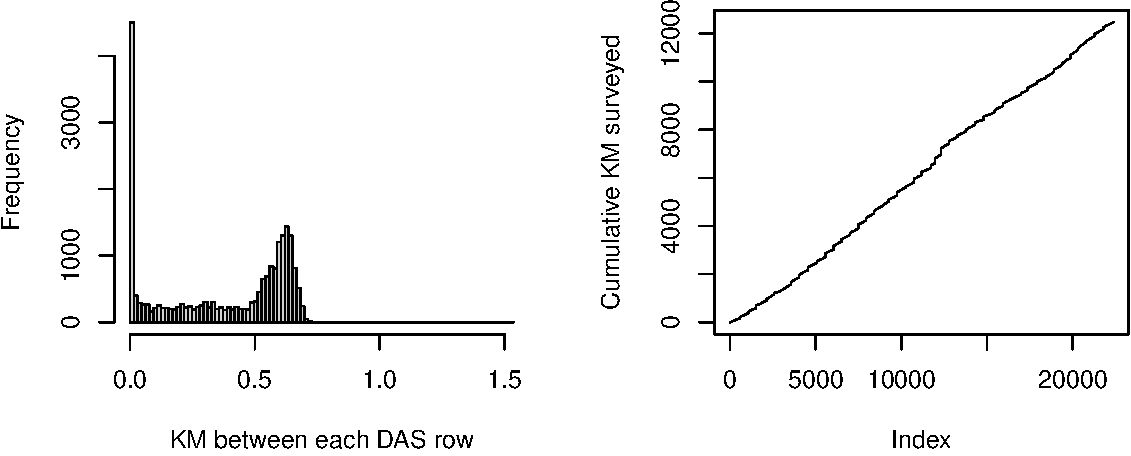
\includegraphics{figures/unnamed-chunk-22-1.pdf}

\hypertarget{process-strata}{%
\section*{Process strata}\label{process-strata}}
\addcontentsline{toc}{section}{Process strata}

Run the following function to add strata and study-area information to each sub-segment of effort:

\begin{Shaded}
\begin{Highlighting}[]
\NormalTok{cruz <-}\StringTok{ }\KeywordTok{process_strata}\NormalTok{(das, settings)}
\NormalTok{Spherical }\KeywordTok{geometry}\NormalTok{ (s2) switched off}
\end{Highlighting}
\end{Shaded}

This function loops through each stratum \texttt{data.frame} you have provided it in \texttt{settings\$strata}, formats the stratum, and asks whether each DAS row occurs within it. For each stratum, a column named \texttt{stratum\_\textless{}StratumName\textgreater{}} is added to the \texttt{das} object; each row in this column is \texttt{TRUE} (included) or \texttt{FALSE}.

A similar procedure is run if a dataframe is provided in \texttt{settings\$study\_area}. A column named \texttt{study\_area} is added to \texttt{das} containing a boolean (\texttt{TRUE} if the sub-segment or sighting occurs within the study area).

The function then loops through each species cohort and uses that cohort's settings to determine a single stratum assignment for each row of \texttt{DAS} data in the event of overlapping strata. The key cohort setting referenced here is \texttt{stratum\_overlap\_handling}.

\hypertarget{the-cruz-object}{%
\subsection*{\texorpdfstring{The \texttt{cruz} object}{The cruz object}}\label{the-cruz-object}}
\addcontentsline{toc}{subsection}{The \texttt{cruz} object}

The function \texttt{process\_strata()} returns a list, which we have saved in an object named \texttt{cruz}, with several slots:

\begin{Shaded}
\begin{Highlighting}[]
\NormalTok{cruz }\OperatorTok\StringTok{ }\NormalTok{names}
\NormalTok{[}\DecValTok{1}\NormalTok{] }\StringTok{"das"}        \StringTok{"settings"}   \StringTok{"strata"}     \StringTok{"study_area"} \StringTok{"cohorts"}   
\end{Highlighting}
\end{Shaded}

The slots \texttt{strata} and \texttt{study\_area} provide the area, in square km, of each polygon being used:

\begin{Shaded}
\begin{Highlighting}[]
\NormalTok{cruz}\OperatorTok{$}\NormalTok{strata}
\NormalTok{   stratum       area}
\DecValTok{1}\NormalTok{   HI_EEZ  }\FloatTok{2491447.3}
\DecValTok{2}\NormalTok{  WHICEAS   }\FloatTok{419789.2}
\DecValTok{3}\NormalTok{ OtherCNP }\FloatTok{34232739.5}
\end{Highlighting}
\end{Shaded}

\begin{Shaded}
\begin{Highlighting}[]
\NormalTok{cruz}\OperatorTok{$}\NormalTok{study_area}
\NormalTok{[}\DecValTok{1}\NormalTok{] }\DecValTok{34232739}
\end{Highlighting}
\end{Shaded}

The slot \texttt{cohorts} is itself a list with one slot for each cohort. The slots are named using the \texttt{id} cohort setting.

\begin{Shaded}
\begin{Highlighting}[]
\NormalTok{cruz}\OperatorTok{$}\NormalTok{cohorts }\OperatorTok\StringTok{ }\NormalTok{names}
\NormalTok{[}\DecValTok{1}\NormalTok{] }\StringTok{"default"}     \StringTok{"fkw_insular"}
\end{Highlighting}
\end{Shaded}

Each cohort slot has a copy of the \texttt{DAS} data with a stratum assignment tailored to its cohort-specific settings. For instance, the \texttt{default} cohort, whose \texttt{stratum\_overlap\_handling} is set to \texttt{"smallest"}, assigns the smallest stratum in the event of overlapping or nested strata:

\begin{Shaded}
\begin{Highlighting}[]
\NormalTok{cruz}\OperatorTok{$}\NormalTok{cohorts}\OperatorTok{$}\NormalTok{default}\OperatorTok{$}\NormalTok{stratum }\OperatorTok\StringTok{ }\KeywordTok{table}\NormalTok{(}\DataTypeTok{useNA=}\StringTok{'ifany'}\NormalTok{)}
\NormalTok{.}
\NormalTok{ HI_EEZ WHICEAS }
    \DecValTok{142}   \DecValTok{22228} 
\end{Highlighting}
\end{Shaded}

The \texttt{fkw\_insular} cohort, whose \texttt{stratum\_overlap\_handling} is set to \texttt{"each"} (i.e., effort is allowed to belong to multiple segments, if they overlap, and all analyses will be conducted for each stratum separately), has stratum assignments that look like this;

\begin{Shaded}
\begin{Highlighting}[]
\NormalTok{cruz}\OperatorTok{$}\NormalTok{cohorts}\OperatorTok{$}\NormalTok{fkw_insular}\OperatorTok{$}\NormalTok{stratum }\OperatorTok\StringTok{ }\KeywordTok{table}\NormalTok{(}\DataTypeTok{useNA=}\StringTok{'ifany'}\NormalTok{)}
\NormalTok{.}
\NormalTok{        HI_EEZ}\OperatorTok{&}\NormalTok{OtherCNP HI_EEZ}\OperatorTok{&}\NormalTok{WHICEAS}\OperatorTok{&}\NormalTok{OtherCNP }
                    \DecValTok{142}                   \DecValTok{22228} 
\end{Highlighting}
\end{Shaded}

When a row of \texttt{DAS} effort occurs in two overlapping strata, the stratum assignment for that row is a concatentation of the names of the strata it falls within, with names separated by ``\texttt{\&}''.

This list, with these five primary slots, will be referred to as a \texttt{cruz} object. The remainder of the data processing work flow is focused upon refining the effort and sighting data for each slot in \texttt{cohorts}. The other slots are no longer modified.

\hypertarget{segmentize-the-data}{%
\section*{Segmentize the data}\label{segmentize-the-data}}
\addcontentsline{toc}{section}{Segmentize the data}

To allocate survey data into discrete `effort segments', which are used in variance estimation in subsequent steps, run the function \texttt{segmentize()}. This process is controlled by both survey-wide and cohort-specific \protect\hypertarget{settings}{}{settings}, which are now carried in a slot within the \texttt{cruz} object.

\begin{Shaded}
\begin{Highlighting}[]
\NormalTok{cruz <-}\StringTok{ }\KeywordTok{segmentize}\NormalTok{(cruz, }\DataTypeTok{verbose=}\OtherTok{TRUE}\NormalTok{)}
\NormalTok{[}\DecValTok{1}\NormalTok{] }\StringTok{"separate"}
\NormalTok{[}\DecValTok{1}\NormalTok{] }\StringTok{"append"}  \StringTok{"segment"}
\NormalTok{[}\DecValTok{1}\NormalTok{] }\StringTok{"equallength"}
\NormalTok{[}\DecValTok{1}\NormalTok{] }\DecValTok{833171}
\NormalTok{[}\DecValTok{1}\NormalTok{] }\DecValTok{172800}
\NormalTok{[}\DecValTok{1}\NormalTok{] }\DecValTok{30}
\NormalTok{[}\DecValTok{1}\NormalTok{] }\StringTok{"S"} \StringTok{"F"}
\NormalTok{[}\DecValTok{1}\NormalTok{] }\StringTok{"P"} \StringTok{"C"}
\NormalTok{[}\DecValTok{1}\NormalTok{] }\OtherTok{TRUE}
\NormalTok{[}\DecValTok{1}\NormalTok{] }\StringTok{"S"} \StringTok{"F"}
\NormalTok{[}\DecValTok{1}\NormalTok{] }\StringTok{"P"} \StringTok{"C"}
\NormalTok{[}\DecValTok{1}\NormalTok{] }\OtherTok{TRUE}
\NormalTok{[}\DecValTok{1}\NormalTok{] }\StringTok{"separate"}
\NormalTok{[}\DecValTok{1}\NormalTok{] }\StringTok{"append"}  \StringTok{"segment"}
\NormalTok{[}\DecValTok{1}\NormalTok{] }\StringTok{"equallength"}
\NormalTok{[}\DecValTok{1}\NormalTok{] }\DecValTok{833171}
\NormalTok{[}\DecValTok{1}\NormalTok{] }\DecValTok{172800}
\NormalTok{[}\DecValTok{1}\NormalTok{] }\DecValTok{30}
\NormalTok{[}\DecValTok{1}\NormalTok{] }\StringTok{"S"} \StringTok{"F"}
\NormalTok{[}\DecValTok{1}\NormalTok{] }\StringTok{"P"} \StringTok{"C"}
\NormalTok{[}\DecValTok{1}\NormalTok{] }\OtherTok{TRUE}
\NormalTok{[}\DecValTok{1}\NormalTok{] }\StringTok{"S"} \StringTok{"F"} \StringTok{"N"}
\NormalTok{[}\DecValTok{1}\NormalTok{] }\StringTok{"P"} \StringTok{"C"}
\NormalTok{[}\DecValTok{1}\NormalTok{] }\OtherTok{TRUE}
\end{Highlighting}
\end{Shaded}

This function does not change the high-level structure of the \texttt{cruz} object \ldots{}

\begin{Shaded}
\begin{Highlighting}[]
\NormalTok{cruz }\OperatorTok\StringTok{ }\NormalTok{names}
\NormalTok{[}\DecValTok{1}\NormalTok{] }\StringTok{"das"}        \StringTok{"settings"}   \StringTok{"strata"}     \StringTok{"study_area"} \StringTok{"cohorts"}   
\end{Highlighting}
\end{Shaded}

\ldots{} or the cohort names in the \texttt{cohorts} slot \ldots{}

\begin{Shaded}
\begin{Highlighting}[]
\NormalTok{cruz}\OperatorTok{$}\NormalTok{cohorts }\OperatorTok\StringTok{ }\NormalTok{names}
\NormalTok{[}\DecValTok{1}\NormalTok{] }\StringTok{"default"}     \StringTok{"fkw_insular"}
\end{Highlighting}
\end{Shaded}

But it \emph{does} change the structure of data within each cohort. Each cohort will now have a slot named \texttt{density} \ldots{}

\begin{Shaded}
\begin{Highlighting}[]
\NormalTok{cruz}\OperatorTok{$}\NormalTok{cohorts}\OperatorTok{$}\NormalTok{default }\OperatorTok\StringTok{ }\NormalTok{names}
\NormalTok{[}\DecValTok{1}\NormalTok{] }\StringTok{"density"}
\end{Highlighting}
\end{Shaded}

And, if your settings specify that settings for density estimation differ from detection function estimation, a cohort will have a second slot named \texttt{distance}. This is the case for the second cohort in our example analysis: \texttt{fkw\_insular}.

\begin{Shaded}
\begin{Highlighting}[]
\NormalTok{cruz}\OperatorTok{$}\NormalTok{cohorts}\OperatorTok{$}\NormalTok{fkw_insular }\OperatorTok\StringTok{ }\NormalTok{names}
\NormalTok{[}\DecValTok{1}\NormalTok{] }\StringTok{"density"}  \StringTok{"distance"}
\end{Highlighting}
\end{Shaded}

Though their data segmentization will differ, the \texttt{density} and \texttt{distance} slots have identical structures:

\begin{Shaded}
\begin{Highlighting}[]
\NormalTok{cruz}\OperatorTok{$}\NormalTok{cohorts}\OperatorTok{$}\NormalTok{fkw_insular}\OperatorTok{$}\NormalTok{density }\OperatorTok\StringTok{ }\NormalTok{names}
\NormalTok{[}\DecValTok{1}\NormalTok{] }\StringTok{"segments"} \StringTok{"effort"}   \StringTok{"das"}     

\NormalTok{cruz}\OperatorTok{$}\NormalTok{cohorts}\OperatorTok{$}\NormalTok{fkw_insular}\OperatorTok{$}\NormalTok{distance }\OperatorTok\StringTok{ }\NormalTok{names}
\NormalTok{[}\DecValTok{1}\NormalTok{] }\StringTok{"segments"} \StringTok{"effort"}   \StringTok{"das"}     
\end{Highlighting}
\end{Shaded}

The \texttt{segments} slot contains summary data for each effort segment, including start/mid/end coordinates, average conditions, and segment distance:

\begin{Shaded}
\begin{Highlighting}[]
\NormalTok{cruz}\OperatorTok{$}\NormalTok{cohorts}\OperatorTok{$}\NormalTok{default}\OperatorTok{$}\NormalTok{density}\OperatorTok{$}\NormalTok{segments }\OperatorTok\StringTok{ }\NormalTok{glimpse}
\NormalTok{Rows}\OperatorTok{:}\StringTok{ }\DecValTok{278}
\NormalTok{Columns}\OperatorTok{:}\StringTok{ }\DecValTok{36}
\OperatorTok{$}\StringTok{ }\NormalTok{Cruise       }\OperatorTok{<}\NormalTok{dbl}\OperatorTok{>}\StringTok{ }\DecValTok{2001}\NormalTok{, }\DecValTok{2001}\NormalTok{, }\DecValTok{2001}\NormalTok{, }\DecValTok{2001}\NormalTok{, }\DecValTok{2001}\NormalTok{, }\DecValTok{2001}\NormalTok{, }\DecValTok{2001}\NormalTok{, }\DecValTok{2001}\NormalTok{, }\DecValTok{2001}\NormalTok{, }\DecValTok{200}\OperatorTok{~}
\ErrorTok{$}\StringTok{ }\NormalTok{stratum      }\OperatorTok{<}\NormalTok{chr}\OperatorTok{>}\StringTok{ "HI_EEZ"}\NormalTok{, }\StringTok{"HI_EEZ"}\NormalTok{, }\StringTok{"HI_EEZ"}\NormalTok{, }\StringTok{"HI_EEZ"}\NormalTok{, }\StringTok{"HI_EEZ"}\NormalTok{, }\StringTok{"WHICEA~}
\StringTok{$ study_area   <lgl> TRUE, TRUE, TRUE, TRUE, TRUE, TRUE, TRUE, TRUE, TRUE, TRU~}
\StringTok{$ seg_id       <int> 1, 2, 3, 4, 5, 6, 7, 8, 9, 10, 11, 12, 13, 14, 15, 16, 17~}
\StringTok{$ yday         <dbl> 21, 22, 39, 68, 22, 19, 19, 19, 20, 20, 21, 22, 23, 23, 2~}
\StringTok{$ dist         <dbl> 3.2237470, 0.6118778, 29.7257476, 19.8973176, 1.2231556, ~}
\StringTok{$ lat1         <dbl> 22.33300, 22.68750, 20.79283, 21.65833, 22.68750, 21.8520~}
\StringTok{$ lon1         <dbl> -161.2520, -161.1208, -153.6117, -161.7810, -161.1208, -1~}
\StringTok{$ DateTime1    <dttm> 2020-01-21 07:28:48, 2020-01-22 07:42:01, 2020-02-08 06:~}
\StringTok{$ timestamp1   <dbl> 1579591728, 1579678921, 1581144814, 1583688255, 157967892~}
\StringTok{$ lat2         <dbl> 22.68750, 20.79217, 21.65683, 21.66717, 22.68617, 22.1771~}
\StringTok{$ lon2         <dbl> -161.1208, -153.6090, -161.7753, -161.9295, -161.1158, -1~}
\StringTok{$ DateTime2    <dttm> 2020-01-22 07:42:01, 2020-02-08 06:51:34, 2020-03-08 17:~}
\StringTok{$ timestamp2   <dbl> 1579678921, 1581144694, 1583688135, 1583692815, 157967903~}
\StringTok{$ mlat         <dbl> 22.69117, 20.79133, 21.62583, 21.68417, 22.68750, 22.2345~}
\StringTok{$ mlon         <dbl> -161.1353, -153.6063, -161.6553, -161.8822, -161.1208, -1~}
\StringTok{$ mDateTime    <dttm> 2020-01-22 07:31:52, 2020-02-08 06:49:34, 2020-03-08 16:~}
\StringTok{$ mtimestamp   <dbl> 1579591728, 1579678921, 1581144814, 1583688255, 157967892~}
\StringTok{$ use          <lgl> FALSE, FALSE, FALSE, FALSE, TRUE, FALSE, FALSE, FALSE, FA~}
\StringTok{$ Mode         <chr> NA, "}\NormalTok{P}\StringTok{", NA, "}\NormalTok{C}\StringTok{", "}\NormalTok{P}\StringTok{", "}\NormalTok{C}\StringTok{", "}\NormalTok{C}\StringTok{", "}\NormalTok{C}\StringTok{", NA, "}\NormalTok{C}\StringTok{", "}\NormalTok{C}\StringTok{", "}\NormalTok{C}\StringTok{", ~}
\StringTok{$ EffType      <chr> NA, "}\NormalTok{S}\StringTok{", NA, "}\NormalTok{S}\StringTok{", "}\NormalTok{S}\StringTok{", NA, "}\NormalTok{N}\StringTok{", "}\NormalTok{F}\StringTok{", NA, "}\NormalTok{S}\StringTok{", "}\NormalTok{F}\StringTok{", "}\NormalTok{S}\StringTok{", "}\OperatorTok{~}
\ErrorTok{$}\StringTok{ }\NormalTok{ESWsides     }\OperatorTok{<}\NormalTok{dbl}\OperatorTok{>}\StringTok{ }\OtherTok{NA}\NormalTok{, }\DecValTok{2}\NormalTok{, }\OtherTok{NA}\NormalTok{, }\DecValTok{2}\NormalTok{, }\DecValTok{2}\NormalTok{, }\OtherTok{NA}\NormalTok{, }\DecValTok{2}\NormalTok{, }\DecValTok{2}\NormalTok{, }\OtherTok{NA}\NormalTok{, }\DecValTok{2}\NormalTok{, }\DecValTok{2}\NormalTok{, }\DecValTok{2}\NormalTok{, }\DecValTok{2}\NormalTok{, }\DecValTok{2}\NormalTok{, }\OtherTok{NA}\NormalTok{, }\DecValTok{2}\NormalTok{, }\DecValTok{2}\NormalTok{, }\DecValTok{2}\OperatorTok{~}
\ErrorTok{$}\StringTok{ }\NormalTok{year         }\OperatorTok{<}\NormalTok{dbl}\OperatorTok{>}\StringTok{ }\DecValTok{2020}\NormalTok{, }\DecValTok{2020}\NormalTok{, }\DecValTok{2020}\NormalTok{, }\DecValTok{2020}\NormalTok{, }\DecValTok{2020}\NormalTok{, }\DecValTok{2020}\NormalTok{, }\DecValTok{2020}\NormalTok{, }\DecValTok{2020}\NormalTok{, }\DecValTok{2020}\NormalTok{, }\DecValTok{202}\OperatorTok{~}
\ErrorTok{$}\StringTok{ }\NormalTok{month        }\OperatorTok{<}\NormalTok{dbl}\OperatorTok{>}\StringTok{ }\DecValTok{1}\NormalTok{, }\DecValTok{1}\NormalTok{, }\DecValTok{2}\NormalTok{, }\DecValTok{3}\NormalTok{, }\DecValTok{1}\NormalTok{, }\DecValTok{1}\NormalTok{, }\DecValTok{1}\NormalTok{, }\DecValTok{1}\NormalTok{, }\DecValTok{1}\NormalTok{, }\DecValTok{1}\NormalTok{, }\DecValTok{1}\NormalTok{, }\DecValTok{1}\NormalTok{, }\DecValTok{1}\NormalTok{, }\DecValTok{1}\NormalTok{, }\DecValTok{1}\NormalTok{, }\DecValTok{1}\NormalTok{, }\DecValTok{1}\NormalTok{, }\DecValTok{1}\NormalTok{, }\DecValTok{1}\NormalTok{, }\OperatorTok{~}
\ErrorTok{$}\StringTok{ }\NormalTok{day          }\OperatorTok{<}\NormalTok{int}\OperatorTok{>}\StringTok{ }\DecValTok{21}\NormalTok{, }\DecValTok{22}\NormalTok{, }\DecValTok{8}\NormalTok{, }\DecValTok{8}\NormalTok{, }\DecValTok{22}\NormalTok{, }\DecValTok{19}\NormalTok{, }\DecValTok{19}\NormalTok{, }\DecValTok{19}\NormalTok{, }\DecValTok{20}\NormalTok{, }\DecValTok{20}\NormalTok{, }\DecValTok{21}\NormalTok{, }\DecValTok{22}\NormalTok{, }\DecValTok{23}\NormalTok{, }\DecValTok{23}\NormalTok{, }\DecValTok{24}\NormalTok{,}\OperatorTok{~}
\ErrorTok{$}\StringTok{ }\NormalTok{min_line     }\OperatorTok{<}\NormalTok{int}\OperatorTok{>}\StringTok{ }\DecValTok{1080}\NormalTok{, }\DecValTok{1549}\NormalTok{, }\DecValTok{9811}\NormalTok{, }\DecValTok{20825}\NormalTok{, }\DecValTok{1550}\NormalTok{, }\DecValTok{11}\NormalTok{, }\DecValTok{240}\NormalTok{, }\DecValTok{601}\NormalTok{, }\DecValTok{701}\NormalTok{, }\DecValTok{963}\NormalTok{, }\DecValTok{14}\OperatorTok{~}
\ErrorTok{$}\StringTok{ }\NormalTok{max_line     }\OperatorTok{<}\NormalTok{int}\OperatorTok{>}\StringTok{ }\DecValTok{1548}\NormalTok{, }\DecValTok{9810}\NormalTok{, }\DecValTok{20824}\NormalTok{, }\DecValTok{20886}\NormalTok{, }\DecValTok{1554}\NormalTok{, }\DecValTok{239}\NormalTok{, }\DecValTok{499}\NormalTok{, }\DecValTok{700}\NormalTok{, }\DecValTok{962}\NormalTok{, }\DecValTok{1486}\NormalTok{,}\OperatorTok{~}
\ErrorTok{$}\StringTok{ }\NormalTok{n_rows       }\OperatorTok{<}\NormalTok{int}\OperatorTok{>}\StringTok{ }\DecValTok{14}\NormalTok{, }\DecValTok{3}\NormalTok{, }\DecValTok{58}\NormalTok{, }\DecValTok{62}\NormalTok{, }\DecValTok{5}\NormalTok{, }\DecValTok{103}\NormalTok{, }\DecValTok{120}\NormalTok{, }\DecValTok{99}\NormalTok{, }\DecValTok{111}\NormalTok{, }\DecValTok{164}\NormalTok{, }\DecValTok{117}\NormalTok{, }\DecValTok{89}\NormalTok{, }\DecValTok{90}\NormalTok{, }\DecValTok{59}\OperatorTok{~}
\ErrorTok{$}\StringTok{ }\NormalTok{avgBft       }\OperatorTok{<}\NormalTok{dbl}\OperatorTok{>}\StringTok{ }\OtherTok{NaN}\NormalTok{, }\OtherTok{NaN}\NormalTok{, }\FloatTok{7.000000}\NormalTok{, }\FloatTok{6.418047}\NormalTok{, }\FloatTok{2.000000}\NormalTok{, }\FloatTok{5.150894}\NormalTok{, }\FloatTok{4.84389}\OperatorTok{~}
\ErrorTok{$}\StringTok{ }\NormalTok{avgSwellHght }\OperatorTok{<}\NormalTok{dbl}\OperatorTok{>}\StringTok{ }\OtherTok{NaN}\NormalTok{, }\OtherTok{NaN}\NormalTok{, }\FloatTok{7.000000}\NormalTok{, }\FloatTok{7.000000}\NormalTok{, }\FloatTok{4.000000}\NormalTok{, }\FloatTok{7.433929}\NormalTok{, }\FloatTok{7.20666}\OperatorTok{~}
\ErrorTok{$}\StringTok{ }\NormalTok{avgHorizSun  }\OperatorTok{<}\NormalTok{dbl}\OperatorTok{>}\StringTok{ }\OtherTok{NaN}\NormalTok{, }\OtherTok{NaN}\NormalTok{, }\FloatTok{10.958794}\NormalTok{, }\FloatTok{11.000000}\NormalTok{, }\OtherTok{NaN}\NormalTok{, }\FloatTok{6.954993}\NormalTok{, }\FloatTok{6.314060}\NormalTok{, }\OperatorTok{~}
\ErrorTok{$}\StringTok{ }\NormalTok{avgVertSun   }\OperatorTok{<}\NormalTok{dbl}\OperatorTok{>}\StringTok{ }\OtherTok{NaN}\NormalTok{, }\OtherTok{NaN}\NormalTok{, }\FloatTok{1.058675}\NormalTok{, }\FloatTok{2.418106}\NormalTok{, }\OtherTok{NaN}\NormalTok{, }\FloatTok{1.419236}\NormalTok{, }\FloatTok{1.178142}\NormalTok{, }\FloatTok{2.}\OperatorTok{~}
\ErrorTok{$}\StringTok{ }\NormalTok{avgGlare     }\OperatorTok{<}\NormalTok{dbl}\OperatorTok{>}\StringTok{ }\OtherTok{NaN}\NormalTok{, }\OtherTok{NaN}\NormalTok{, }\FloatTok{0.05867486}\NormalTok{, }\FloatTok{1.00000000}\NormalTok{, }\OtherTok{NaN}\NormalTok{, }\FloatTok{0.00000000}\NormalTok{, }\FloatTok{0.4734}\OperatorTok{~}
\ErrorTok{$}\StringTok{ }\NormalTok{avgVis       }\OperatorTok{<}\NormalTok{dbl}\OperatorTok{>}\StringTok{ }\FloatTok{4.000000}\NormalTok{, }\OtherTok{NaN}\NormalTok{, }\FloatTok{5.000000}\NormalTok{, }\FloatTok{4.709023}\NormalTok{, }\FloatTok{6.200000}\NormalTok{, }\FloatTok{5.641518}\NormalTok{, }\FloatTok{6.}\OperatorTok{~}
\ErrorTok{$}\StringTok{ }\NormalTok{avgCourse    }\OperatorTok{<}\NormalTok{dbl}\OperatorTok{>}\StringTok{ }\OtherTok{NaN}\NormalTok{, }\OtherTok{NaN}\NormalTok{, }\FloatTok{287.23315}\NormalTok{, }\FloatTok{269.55972}\NormalTok{, }\FloatTok{105.00000}\NormalTok{, }\FloatTok{247.16155}\NormalTok{, }\DecValTok{166}\OperatorTok{~}
\ErrorTok{$}\StringTok{ }\NormalTok{avgSpdKt     }\OperatorTok{<}\NormalTok{dbl}\OperatorTok{>}\StringTok{ }\OtherTok{NaN}\NormalTok{, }\OtherTok{NaN}\NormalTok{, }\FloatTok{9.968032}\NormalTok{, }\FloatTok{9.315076}\NormalTok{, }\FloatTok{9.000000}\NormalTok{, }\FloatTok{8.964329}\NormalTok{, }\FloatTok{8.18859}\OperatorTok{~}
\end{Highlighting}
\end{Shaded}

\begin{Shaded}
\begin{Highlighting}[]
\CommentTok{# Number of segments}
\NormalTok{cruz}\OperatorTok{$}\NormalTok{cohorts}\OperatorTok{$}\NormalTok{default}\OperatorTok{$}\NormalTok{density}\OperatorTok{$}\NormalTok{segments }\OperatorTok\StringTok{ }\NormalTok{nrow}
\NormalTok{[}\DecValTok{1}\NormalTok{] }\DecValTok{278}

\CommentTok{# Segment length distribution}
\KeywordTok{hist}\NormalTok{(cruz}\OperatorTok{$}\NormalTok{cohorts}\OperatorTok{$}\NormalTok{default}\OperatorTok{$}\NormalTok{density}\OperatorTok{$}\NormalTok{segments}\OperatorTok{$}\NormalTok{dist,}
     \DataTypeTok{breaks =} \KeywordTok{seq}\NormalTok{(}\DecValTok{0}\NormalTok{,}\DecValTok{60}\NormalTok{,}\DataTypeTok{by=}\DecValTok{1}\NormalTok{),}
     \DataTypeTok{xlab=}\StringTok{'Segment lengths (km)'}\NormalTok{,}
     \DataTypeTok{main=}\KeywordTok{paste0}\NormalTok{(}\StringTok{'Target km: '}\NormalTok{,settings}\OperatorTok{$}\NormalTok{survey}\OperatorTok{$}\NormalTok{segment_target_km))}
\end{Highlighting}
\end{Shaded}

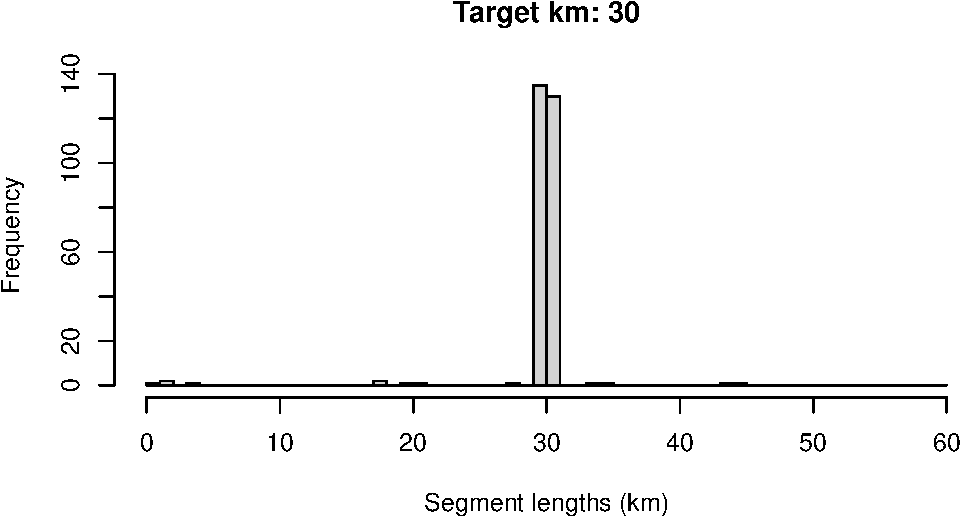
\includegraphics{figures/unnamed-chunk-37-1.pdf}

The \texttt{effort} slot is itself a list in which each slot holds the \texttt{DAS} for a single segment.

\begin{Shaded}
\begin{Highlighting}[]
\NormalTok{cruz}\OperatorTok{$}\NormalTok{cohorts}\OperatorTok{$}\NormalTok{default}\OperatorTok{$}\NormalTok{density}\OperatorTok{$}\NormalTok{effort }\OperatorTok\StringTok{ }\NormalTok{length}
\NormalTok{[}\DecValTok{1}\NormalTok{] }\DecValTok{278}
\end{Highlighting}
\end{Shaded}

And the \texttt{das} slot holds the original \texttt{data.frame} of \texttt{DAS} data, modified slightly: the column \texttt{OnEffort} has been modified according to Beaufort range conditions, and the column \texttt{seg\_id} indicates which segment the event occurs within

\begin{Shaded}
\begin{Highlighting}[]
\NormalTok{cruz}\OperatorTok{$}\NormalTok{cohorts}\OperatorTok{$}\NormalTok{default}\OperatorTok{$}\NormalTok{density}\OperatorTok{$}\NormalTok{das }\OperatorTok\StringTok{ }\NormalTok{names}
\NormalTok{ [}\DecValTok{1}\NormalTok{] }\StringTok{"Event"}            \StringTok{"DateTime"}         \StringTok{"Lat"}              \StringTok{"Lon"}             
\NormalTok{ [}\DecValTok{5}\NormalTok{] }\StringTok{"OnEffort"}         \StringTok{"Cruise"}           \StringTok{"Mode"}             \StringTok{"OffsetGMT"}       
\NormalTok{ [}\DecValTok{9}\NormalTok{] }\StringTok{"EffType"}          \StringTok{"ESWsides"}         \StringTok{"Course"}           \StringTok{"SpdKt"}           
\NormalTok{[}\DecValTok{13}\NormalTok{] }\StringTok{"Bft"}              \StringTok{"SwellHght"}        \StringTok{"WindSpdKt"}        \StringTok{"RainFog"}         
\NormalTok{[}\DecValTok{17}\NormalTok{] }\StringTok{"HorizSun"}         \StringTok{"VertSun"}          \StringTok{"Glare"}            \StringTok{"Vis"}             
\NormalTok{[}\DecValTok{21}\NormalTok{] }\StringTok{"ObsL"}             \StringTok{"Rec"}              \StringTok{"ObsR"}             \StringTok{"ObsInd"}          
\NormalTok{[}\DecValTok{25}\NormalTok{] }\StringTok{"Data1"}            \StringTok{"Data2"}            \StringTok{"Data3"}            \StringTok{"Data4"}           
\NormalTok{[}\DecValTok{29}\NormalTok{] }\StringTok{"Data5"}            \StringTok{"Data6"}            \StringTok{"Data7"}            \StringTok{"Data8"}           
\NormalTok{[}\DecValTok{33}\NormalTok{] }\StringTok{"Data9"}            \StringTok{"Data10"}           \StringTok{"Data11"}           \StringTok{"Data12"}          
\NormalTok{[}\DecValTok{37}\NormalTok{] }\StringTok{"EffortDot"}        \StringTok{"EventNum"}         \StringTok{"file_das"}         \StringTok{"line_num"}        
\NormalTok{[}\DecValTok{41}\NormalTok{] }\StringTok{"year"}             \StringTok{"month"}            \StringTok{"day"}              \StringTok{"yday"}            
\NormalTok{[}\DecValTok{45}\NormalTok{] }\StringTok{"km_int"}           \StringTok{"km_cum"}           \StringTok{"stratum_HI_EEZ"}   \StringTok{"stratum_WHICEAS"} 
\NormalTok{[}\DecValTok{49}\NormalTok{] }\StringTok{"stratum_OtherCNP"} \StringTok{"study_area"}       \StringTok{"stratum"}          \StringTok{"seg_id"}          
\end{Highlighting}
\end{Shaded}

The \texttt{segmentize()} function and its associated settings were designed to give researchers full control over how data are segmented, be it for design-based density analysis (which tend to use long segments of 100 km or more and allow for non-contiguous effort to be included in the same segment) or for habitat modeling (which tend to use short segments of 5 - 10 km and disallow non-contiguous effort to be pooled into the same segment). To demonstrate that versatility, checkout the \protect\hyperlink{segmentizing}{appendix on segmentizing}.

\hypertarget{process-sightings}{%
\section*{Process sightings}\label{process-sightings}}
\addcontentsline{toc}{section}{Process sightings}

\emph{Coming soon!}

\hypertarget{maps}{%
\chapter{Maps}\label{maps}}

To build a flexible system for mapping cruise data, we have the following functions:

\hypertarget{base-maps}{%
\section*{Base maps}\label{base-maps}}
\addcontentsline{toc}{section}{Base maps}

Begin with a basic map, including EEZ borders:

\begin{Shaded}
\begin{Highlighting}[]
\NormalTok{m <-}\StringTok{ }\KeywordTok{map_base}\NormalTok{(}\DataTypeTok{region=}\StringTok{'cnp'}\NormalTok{)}
\NormalTok{m}
\end{Highlighting}
\end{Shaded}

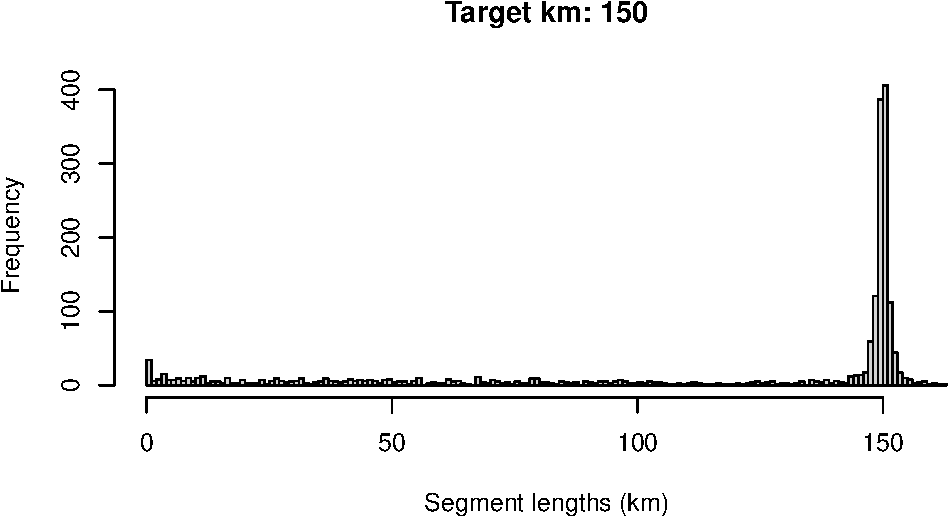
\includegraphics{figures/unnamed-chunk-43-1.pdf}

We also have a base map for the California Current \ldots{}

\begin{Shaded}
\begin{Highlighting}[]
\NormalTok{m <-}\StringTok{ }\KeywordTok{map_base}\NormalTok{(}\DataTypeTok{region=}\StringTok{'ccs'}\NormalTok{)}
\NormalTok{m}
\end{Highlighting}
\end{Shaded}

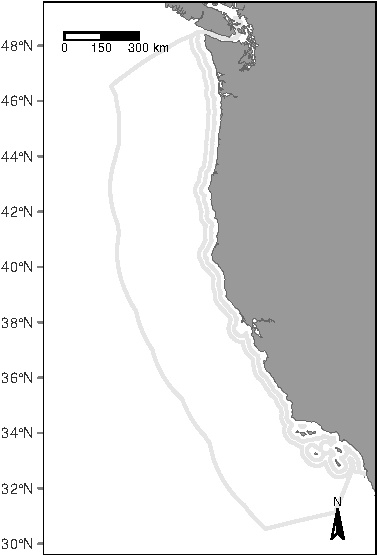
\includegraphics{figures/unnamed-chunk-44-1.pdf}

And the ETP:

\begin{Shaded}
\begin{Highlighting}[]
\NormalTok{m <-}\StringTok{ }\KeywordTok{map_base}\NormalTok{(}\DataTypeTok{region=}\StringTok{'etp'}\NormalTok{)}
\NormalTok{m}
\end{Highlighting}
\end{Shaded}

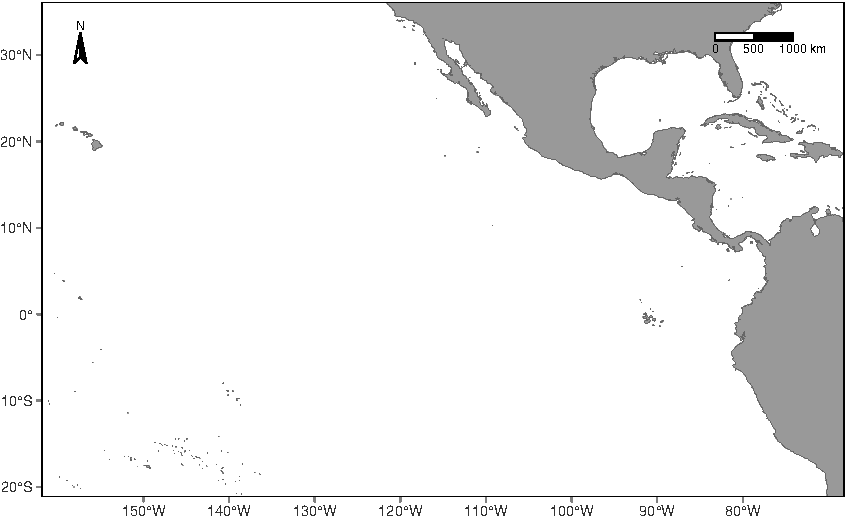
\includegraphics{figures/unnamed-chunk-45-1.pdf}

\hypertarget{add-strata}{%
\section*{Add strata}\label{add-strata}}
\addcontentsline{toc}{section}{Add strata}

Add your research strata to your map:

\begin{Shaded}
\begin{Highlighting}[]
\NormalTok{m <-}\StringTok{ }\KeywordTok{map_base}\NormalTok{(}\DataTypeTok{region=}\StringTok{'cnp'}\NormalTok{)}
\NormalTok{m <-}\StringTok{ }\KeywordTok{map_strata}\NormalTok{(m, }
\NormalTok{                settings, }
                \DataTypeTok{region=}\StringTok{'cnp'}\NormalTok{)}
\NormalTok{m}
\end{Highlighting}
\end{Shaded}

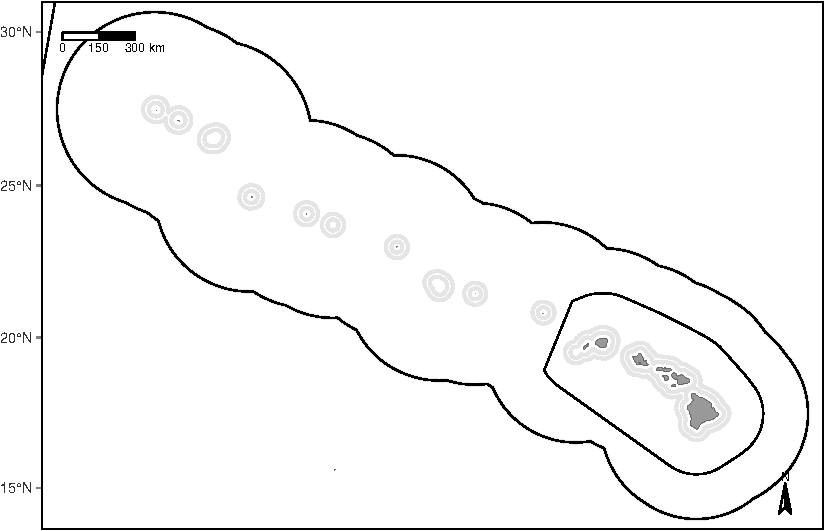
\includegraphics{figures/unnamed-chunk-46-1.pdf}

\hypertarget{add-survey-tracks}{%
\section*{Add survey tracks}\label{add-survey-tracks}}
\addcontentsline{toc}{section}{Add survey tracks}

\emph{Note: this may take a minute to render.}

\begin{Shaded}
\begin{Highlighting}[]
\NormalTok{m1 <-}\StringTok{ }\KeywordTok{map_effort}\NormalTok{(m, cruz)}
\NormalTok{m1}
\end{Highlighting}
\end{Shaded}

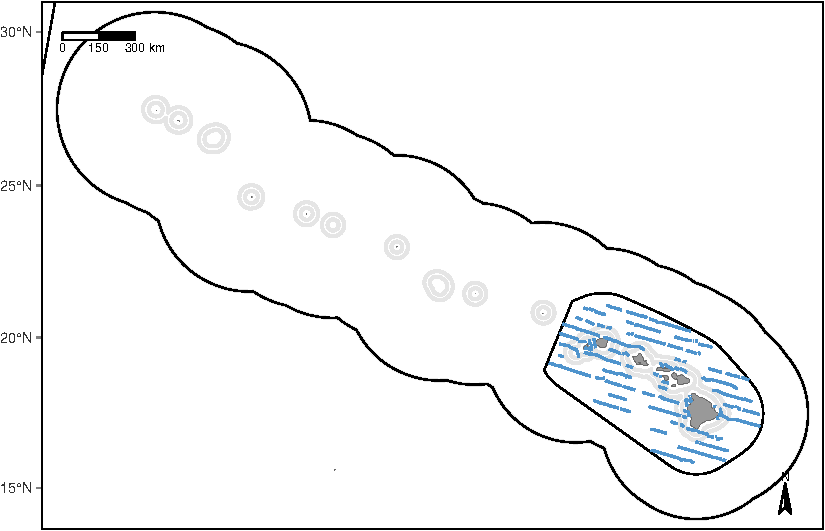
\includegraphics{figures/unnamed-chunk-47-1.pdf}

The defaults of \texttt{map\_effort()} assume, for simplicity, that you want to see the segments to be included in density estimation for the first cohort specified in your settings. You can adjust this and other defaults using the function arguments.

\hypertarget{customizing-effort}{%
\section*{Customizing effort}\label{customizing-effort}}
\addcontentsline{toc}{section}{Customizing effort}

\hypertarget{inputs}{%
\subsection*{Inputs}\label{inputs}}
\addcontentsline{toc}{subsection}{Inputs}

To demonstrate some of the customization options, consider this map that shows segments to be \emph{excluded} from the \texttt{"distance"} (detection function) analysis for our second cohort (\texttt{fkw\_insular}).

\begin{Shaded}
\begin{Highlighting}[]
\KeywordTok{map_effort}\NormalTok{(m, cruz,}
           \DataTypeTok{cohort =} \DecValTok{2}\NormalTok{,}
           \DataTypeTok{analysis =} \StringTok{'distance'}\NormalTok{,}
           \DataTypeTok{use_type =} \KeywordTok{c}\NormalTok{(}\OtherTok{FALSE}\NormalTok{),}
           \DataTypeTok{effort_color=}\StringTok{'firebrick'}\NormalTok{,}
           \DataTypeTok{effort_stroke=}\FloatTok{2.5}\NormalTok{,}
           \DataTypeTok{effort_linetype=}\DecValTok{1}\NormalTok{,)}
\end{Highlighting}
\end{Shaded}

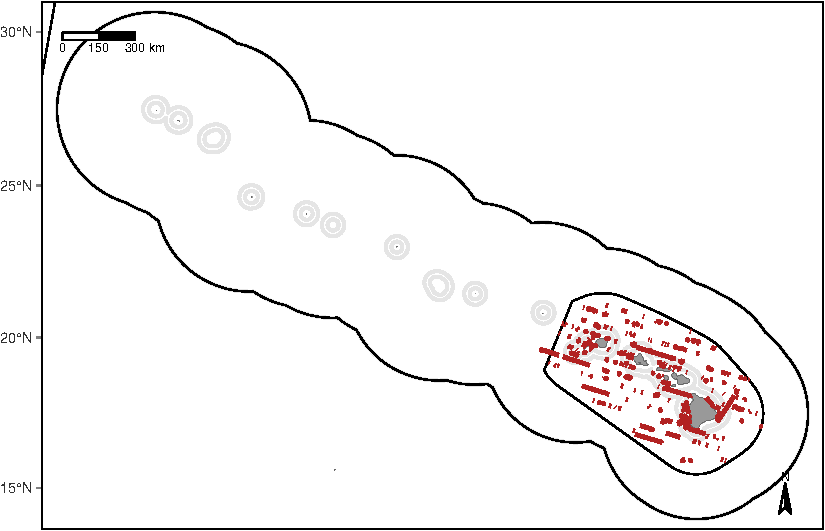
\includegraphics{figures/unnamed-chunk-48-1.pdf}

\hypertarget{color-code-conditions}{%
\subsection*{Color-code conditions}\label{color-code-conditions}}
\addcontentsline{toc}{subsection}{Color-code conditions}

Your second customization option is to add format variables to the \texttt{segments} slot of the cohort of interest in the \texttt{cruz} object. This gives you full control of line color, thickness, and line-type according to whatever specifications you wish to set, e.g., color-coding by effort type or Beaufort sea state.

This is possible because the function \texttt{map\_effort()} looks for the variables \texttt{col} (line color), \texttt{lwd} (line thickness or stroke), and \texttt{lty} (line type) in the columns of \texttt{cruz\$segments}. If these columns exist, the values therein will be used instead of the function defaults.

For example, color-code by Beaufort scale:

\begin{Shaded}
\begin{Highlighting}[]
\CommentTok{# Save copy of cruz object data to modify}
\NormalTok{cruz2 <-}\StringTok{ }\NormalTok{cruz}
\NormalTok{segments <-}\StringTok{ }\NormalTok{cruz2}\OperatorTok{$}\NormalTok{cohorts}\OperatorTok{$}\NormalTok{default}\OperatorTok{$}\NormalTok{density}\OperatorTok{$}\NormalTok{segments}

\CommentTok{# Add column `col`: color code by BFT sea state}
\NormalTok{bft_colors <-}\StringTok{ }\KeywordTok{c}\NormalTok{(}\StringTok{'steelblue4'}\NormalTok{,}\StringTok{'steelblue2'}\NormalTok{,}\StringTok{'cadetblue1'}\NormalTok{,}\StringTok{'grey'}\NormalTok{)}
\NormalTok{segments}\OperatorTok{$}\NormalTok{col <-}\StringTok{ }\NormalTok{bft_colors[}\DecValTok{4}\NormalTok{]}
\NormalTok{segments}\OperatorTok{$}\NormalTok{col[ segments}\OperatorTok{$}\NormalTok{avgBft }\OperatorTok{<=}\StringTok{ }\DecValTok{7}\NormalTok{ ] <-}\StringTok{ }\NormalTok{bft_colors[}\DecValTok{3}\NormalTok{] }\CommentTok{# bft 5 +}
\NormalTok{segments}\OperatorTok{$}\NormalTok{col[ segments}\OperatorTok{$}\NormalTok{avgBft }\OperatorTok{<=}\StringTok{ }\DecValTok{4}\NormalTok{ ] <-}\StringTok{ }\NormalTok{bft_colors[}\DecValTok{2}\NormalTok{] }\CommentTok{# bft 3 - 4}
\NormalTok{segments}\OperatorTok{$}\NormalTok{col[ segments}\OperatorTok{$}\NormalTok{avgBft }\OperatorTok{<=}\StringTok{ }\DecValTok{2}\NormalTok{ ] <-}\StringTok{ }\NormalTok{bft_colors[}\DecValTok{1}\NormalTok{] }\CommentTok{# bft 0 -2}

\CommentTok{# Update sub_segments slot in `cruz` object}
\NormalTok{cruz2}\OperatorTok{$}\NormalTok{cohorts}\OperatorTok{$}\NormalTok{default}\OperatorTok{$}\NormalTok{density}\OperatorTok{$}\NormalTok{segments <-}\StringTok{ }\NormalTok{segments}

\CommentTok{# Update map }
\NormalTok{m_custom2 <-}\StringTok{ }\KeywordTok{map_effort}\NormalTok{(m, cruz2)}

\CommentTok{# Add legend using native functions from mapping package `tmap`}
\NormalTok{m_custom2 <-}\StringTok{ }
\StringTok{  }\NormalTok{m_custom2 }\OperatorTok{+}\StringTok{ }
\StringTok{  }\NormalTok{tmap}\OperatorTok{::}\KeywordTok{tm_add_legend}\NormalTok{(}\StringTok{'line'}\NormalTok{, }
                        \DataTypeTok{col =}\NormalTok{ bft_colors,}
                        \DataTypeTok{lwd =} \DecValTok{3}\NormalTok{,}
                        \DataTypeTok{labels =} \KeywordTok{c}\NormalTok{(}\StringTok{' 0 - 2'}\NormalTok{, }
                                   \StringTok{' 3 - 4'}\NormalTok{, }
                                   \StringTok{' 5 +'}\NormalTok{, }
                                   \StringTok{' no data'}\NormalTok{),}
                         \DataTypeTok{title=}\StringTok{"Beaufort sea state"}\NormalTok{) }\OperatorTok{+}
\StringTok{  }\NormalTok{tmap}\OperatorTok{::}\KeywordTok{tm_layout}\NormalTok{(}\DataTypeTok{legend.position=}\KeywordTok{c}\NormalTok{(}\StringTok{'left'}\NormalTok{,}\StringTok{'bottom'}\NormalTok{))}

\CommentTok{# Show map}
\NormalTok{m_custom2}
\end{Highlighting}
\end{Shaded}

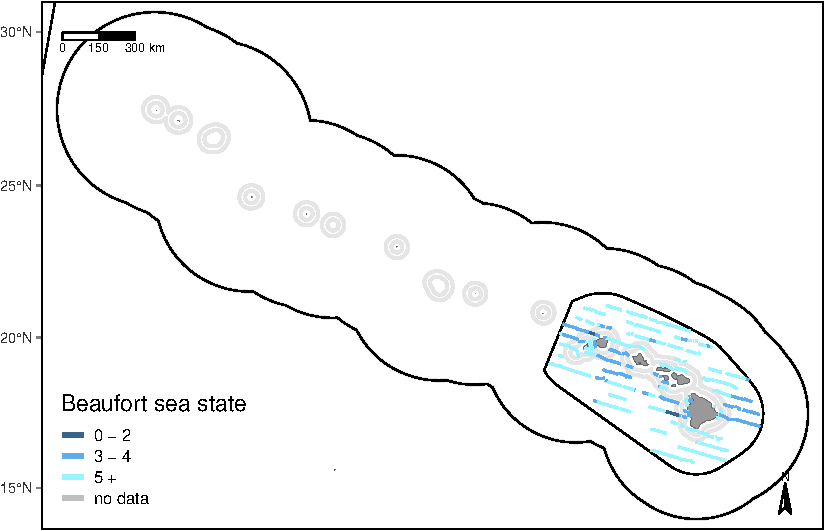
\includegraphics{figures/unnamed-chunk-49-1.pdf}

\hypertarget{summarize}{%
\chapter{Summarize survey}\label{summarize}}

\emph{Coming soon!}

\hypertarget{df}{%
\chapter{Detection functions}\label{df}}

\emph{Coming soon!}

\hypertarget{abundance}{%
\chapter{Abundance estimation}\label{abundance}}

\emph{Coming soon!}

\hypertarget{casestudies}{%
\chapter{Case studies}\label{casestudies}}

To demonstrate what we are building, below is template for quickly running all of the steps detailed in subsequent chapters.

\hypertarget{central-north-pacific}{%
\section*{Central North Pacific}\label{central-north-pacific}}
\addcontentsline{toc}{section}{Central North Pacific}

This template use the same data and settings used throughout the vignette:

\begin{Shaded}
\begin{Highlighting}[]
\KeywordTok{library}\NormalTok{(LTabundR)}

\CommentTok{# Settings =====================================================================}

\CommentTok{# Load strata & study area}
\KeywordTok{data}\NormalTok{(strata_cnp)}
\KeywordTok{data}\NormalTok{(study_cnp)}

\CommentTok{# Survey-wide}
\NormalTok{survey <-}\StringTok{ }
\StringTok{  }\KeywordTok{load_survey_settings}\NormalTok{(}\DataTypeTok{segment_method =} \StringTok{'equallength'}\NormalTok{,}
                       \DataTypeTok{segment_target_km =} \DecValTok{30}\NormalTok{,}
                       \DataTypeTok{segment_max_km_gap =} \DecValTok{5}\NormalTok{,}
                       \DataTypeTok{segment_max_interval =} \DecValTok{48}\NormalTok{,}
                       \DataTypeTok{segment_type_handling =} \StringTok{'separate'}\NormalTok{,}
                       \DataTypeTok{segment_remainder_handling =} \KeywordTok{c}\NormalTok{(}\StringTok{'append'}\NormalTok{,}\StringTok{'segment'}\NormalTok{),}
                       \DataTypeTok{verbose =} \OtherTok{TRUE}\NormalTok{)}

\CommentTok{# Cohort 1 (default)}
\NormalTok{cohort1 <-}\StringTok{ }\KeywordTok{load_cohort_settings}\NormalTok{()}

\CommentTok{# Cohort 2}
\NormalTok{cohort2 <-}\StringTok{ }
\StringTok{  }\KeywordTok{load_cohort_settings}\NormalTok{(}\DataTypeTok{id=}\StringTok{'fkw_insular'}\NormalTok{,}
                       \DataTypeTok{species=}\DecValTok{33}\NormalTok{,}
                       \DataTypeTok{use_low_if_na =} \OtherTok{TRUE}\NormalTok{,}
                       \DataTypeTok{truncation_km =} \DecValTok{5}\NormalTok{,}
                       \DataTypeTok{strata_overlap_handling =} \StringTok{'each'}\NormalTok{)}

\CommentTok{# Finalize settings}
\NormalTok{settings <-}\StringTok{ }\KeywordTok{load_settings}\NormalTok{(}\DataTypeTok{strata =}\NormalTok{ strata_cnp,}
                          \DataTypeTok{study_area =}\NormalTok{ study_cnp,}
                          \DataTypeTok{survey =}\NormalTok{ survey,}
                          \DataTypeTok{cohorts=}\KeywordTok{list}\NormalTok{(cohort1,}
\NormalTok{                                       cohort2))}


\CommentTok{# Processing ===================================================================}

\CommentTok{# Load & format DAS}
\NormalTok{das_file <-}\StringTok{ 'data/surveys/HICEASwinter2020.das'}
\NormalTok{das <-}\StringTok{ }\KeywordTok{load_das}\NormalTok{(das_file, }
                \DataTypeTok{perform_checks =} \OtherTok{TRUE}\NormalTok{,}
                \DataTypeTok{print_glimpse =} \OtherTok{TRUE}\NormalTok{)}
\NormalTok{das <-}\StringTok{ }\KeywordTok{format_das}\NormalTok{(das, settings)}

\CommentTok{# Process strata}
\NormalTok{cruz <-}\StringTok{ }\KeywordTok{process_strata}\NormalTok{(das, settings)}

\CommentTok{# Sanity-check stratum assignments}
\NormalTok{cruz}\OperatorTok{$}\NormalTok{cohorts}\OperatorTok{$}\NormalTok{default}\OperatorTok{$}\NormalTok{stratum }\OperatorTok\StringTok{ }\KeywordTok{table}\NormalTok{(}\DataTypeTok{useNA=}\StringTok{'ifany'}\NormalTok{)}
\NormalTok{cruz}\OperatorTok{$}\NormalTok{cohorts}\OperatorTok{$}\NormalTok{fkw_insular}\OperatorTok{$}\NormalTok{stratum }\OperatorTok\StringTok{ }\KeywordTok{table}\NormalTok{(}\DataTypeTok{useNA=}\StringTok{'ifany'}\NormalTok{)}

\CommentTok{# Segmentize}
\NormalTok{cruz <-}\StringTok{ }\KeywordTok{segmentize}\NormalTok{(cruz, }\DataTypeTok{verbose=}\OtherTok{TRUE}\NormalTok{)}

\CommentTok{# Review: Number of segments}
\NormalTok{cruz}\OperatorTok{$}\NormalTok{cohorts}\OperatorTok{$}\NormalTok{default}\OperatorTok{$}\NormalTok{density}\OperatorTok{$}\NormalTok{segments }\OperatorTok\StringTok{ }\NormalTok{nrow}

\CommentTok{# Review: segment length distribution}
\KeywordTok{hist}\NormalTok{(cruz}\OperatorTok{$}\NormalTok{cohorts}\OperatorTok{$}\NormalTok{default}\OperatorTok{$}\NormalTok{density}\OperatorTok{$}\NormalTok{segments}\OperatorTok{$}\NormalTok{dist,}
     \DataTypeTok{breaks =} \KeywordTok{seq}\NormalTok{(}\DecValTok{0}\NormalTok{,}\DecValTok{60}\NormalTok{,}\DataTypeTok{by=}\DecValTok{1}\NormalTok{),}
     \DataTypeTok{xlab=}\StringTok{'Segment lengths (km)'}\NormalTok{,}
     \DataTypeTok{main=}\KeywordTok{paste0}\NormalTok{(}\StringTok{'Target km: '}\NormalTok{,settings}\OperatorTok{$}\NormalTok{survey}\OperatorTok{$}\NormalTok{segment_target_km))}
\end{Highlighting}
\end{Shaded}

\hypertarget{california-current-system}{%
\section*{California Current System}\label{california-current-system}}
\addcontentsline{toc}{section}{California Current System}

\begin{Shaded}
\begin{Highlighting}[]
\KeywordTok{library}\NormalTok{(LTabundR)}

\CommentTok{# Read in DAS data}
\NormalTok{das_file <-}\StringTok{ 'data/surveys/CAORWA_91-09.das'}
\NormalTok{das <-}\StringTok{ }\KeywordTok{load_das}\NormalTok{(das_file)}

\CommentTok{# Subset to a single cruise}
\NormalTok{das <-}\StringTok{ }\NormalTok{das }\OperatorTok\StringTok{ }\KeywordTok{filter}\NormalTok{(Cruise }\OperatorTok{==}\StringTok{ }\DecValTok{1635}\NormalTok{)}
\end{Highlighting}
\end{Shaded}

\hypertarget{eastern-tropical-pacific}{%
\section*{Eastern Tropical Pacific}\label{eastern-tropical-pacific}}
\addcontentsline{toc}{section}{Eastern Tropical Pacific}

\hypertarget{practicalities}{%
\chapter{Practicalities}\label{practicalities}}

\hypertarget{reproducibility-project-management}{%
\subsection*{Reproducibility \& project management}\label{reproducibility-project-management}}
\addcontentsline{toc}{subsection}{Reproducibility \& project management}

One of the features of the \texttt{ABUND} framework we need to retain is that each analysis is self-contained and reproducible. The folder for an analysis must have all the files and data needed for someone else to be able to replicate it.

In the \texttt{R} package framework we are developing, the contents of a project folder will be straightforward (once the code base is bundled into a package).

\emph{Contents of a project folder:}

\begin{itemize}
\tightlist
\item
  \texttt{DAS} file(s) with survey data\\
\item
  Stratum and study area polygon(s), as \texttt{csv}(s) (optional)\\
\item
  Group size calibration files (optional)\\
\item
  An \texttt{analysis.R} file (or perhaps a \texttt{.Rmd}), containing an adaptation of the code provided in the template above. This script will contain project-specific settings (e.g., the \texttt{load\_settings()} call), which allow for the script to be reproducible.
\end{itemize}

\hypertarget{stratagallery}{%
\chapter{Appendix: Strata gallery}\label{stratagallery}}

\hypertarget{central-north-pacific-1}{%
\section*{Central North Pacific}\label{central-north-pacific-1}}
\addcontentsline{toc}{section}{Central North Pacific}

\begin{Shaded}
\begin{Highlighting}[]
\KeywordTok{strata_explore}\NormalTok{(}\StringTok{'cnp'}\NormalTok{)}
\end{Highlighting}
\end{Shaded}

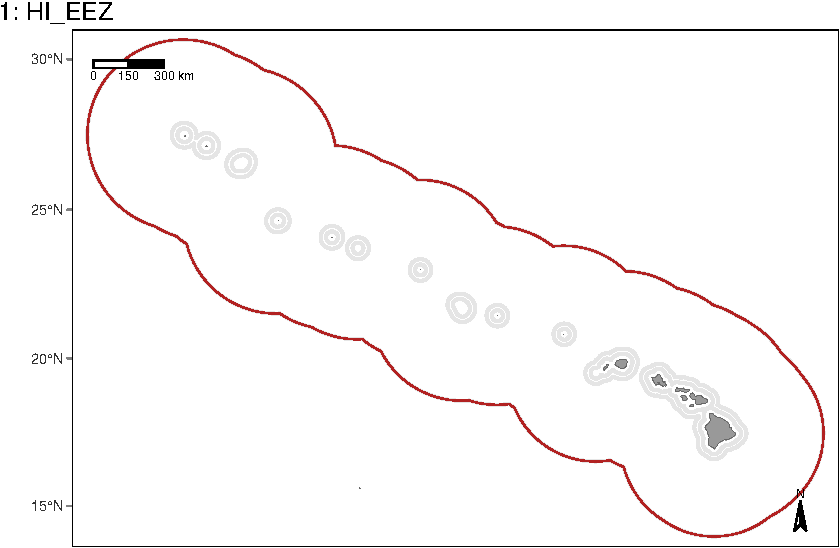
\includegraphics{figures/unnamed-chunk-53-1.pdf} 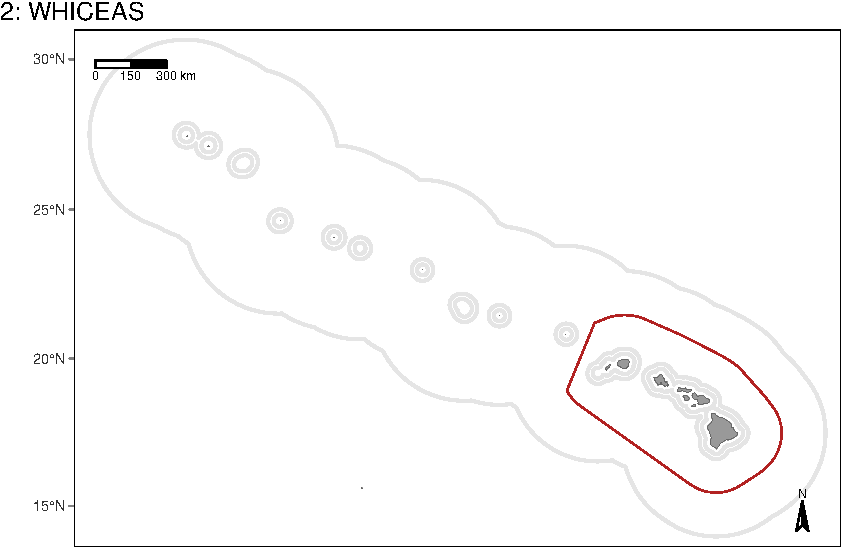
\includegraphics{figures/unnamed-chunk-53-2.pdf} 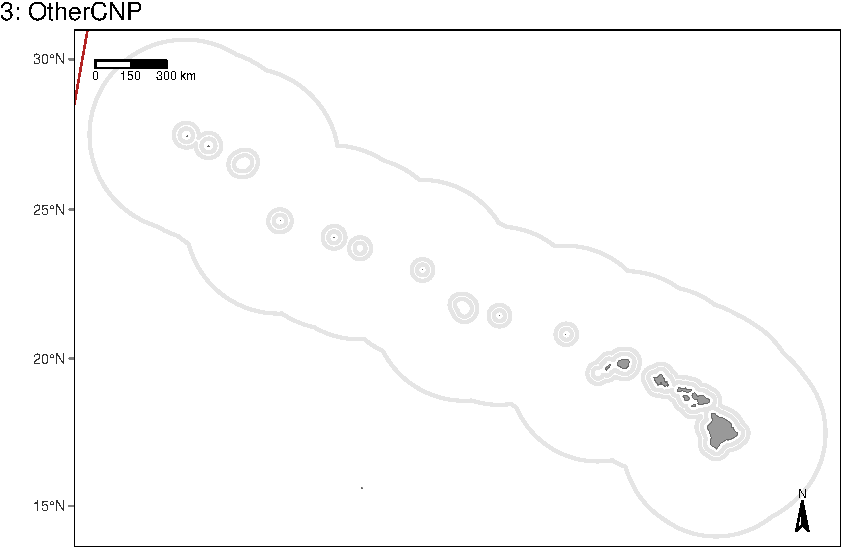
\includegraphics{figures/unnamed-chunk-53-3.pdf}

To acquire the filepath to one of these strata, pass the index (or indices) printed in the map titles above to the function \texttt{strata\_select()}:

\begin{Shaded}
\begin{Highlighting}[]
\NormalTok{strata <-}\StringTok{ }\KeywordTok{strata_select}\NormalTok{(}\DataTypeTok{selections =} \KeywordTok{c}\NormalTok{(}\DecValTok{1}\NormalTok{,}\DecValTok{3}\NormalTok{),}
                              \DataTypeTok{region =} \StringTok{'cnp'}\NormalTok{)}
\end{Highlighting}
\end{Shaded}

This function returns a named list that can be passed directly to the \texttt{strata} argument in \texttt{load\_settings()}.

\begin{Shaded}
\begin{Highlighting}[]
\NormalTok{strata }\OperatorTok\StringTok{ }\NormalTok{names}
\NormalTok{[}\DecValTok{1}\NormalTok{] }\StringTok{"HI_EEZ"}   \StringTok{"OtherCNP"}
\end{Highlighting}
\end{Shaded}

The second slot, \texttt{\$paths}, contains the filepaths you would need to pass to the \texttt{load\_settings()} function.

\hypertarget{california-current}{%
\section*{California Current}\label{california-current}}
\addcontentsline{toc}{section}{California Current}

\begin{Shaded}
\begin{Highlighting}[]
\KeywordTok{strata_explore}\NormalTok{(}\StringTok{'ccs'}\NormalTok{)}
\end{Highlighting}
\end{Shaded}

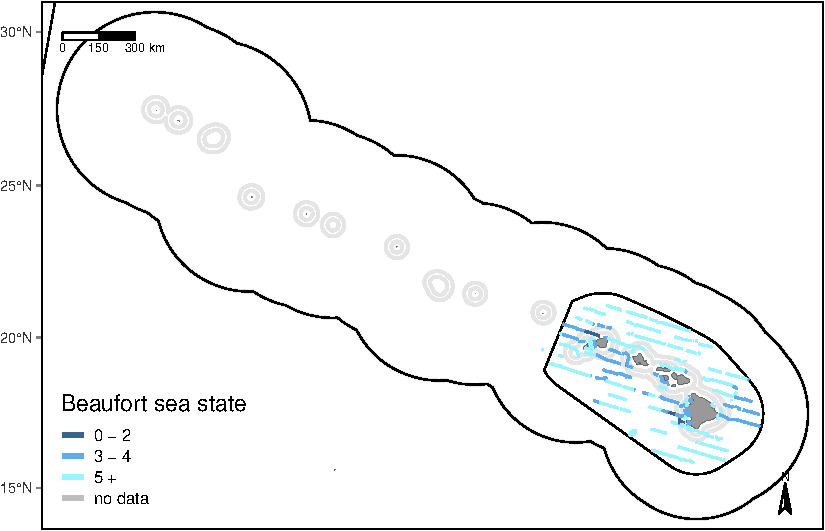
\includegraphics{figures/unnamed-chunk-56-1.pdf} 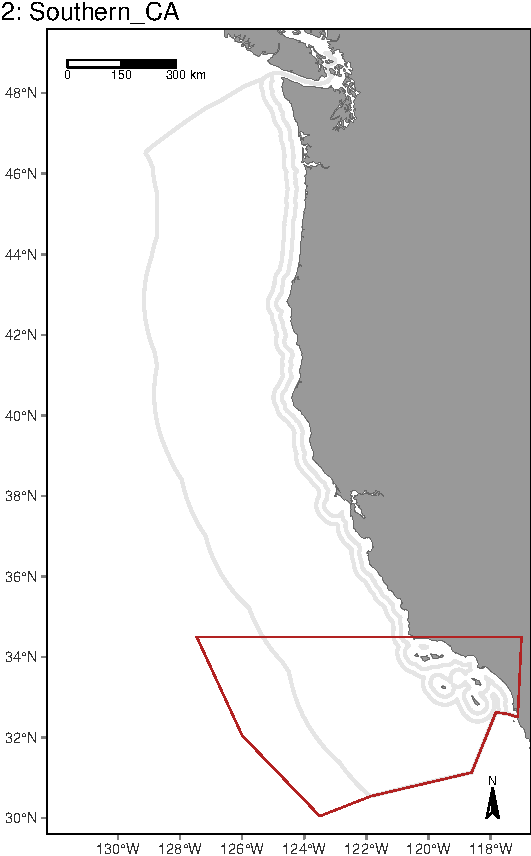
\includegraphics{figures/unnamed-chunk-56-2.pdf} 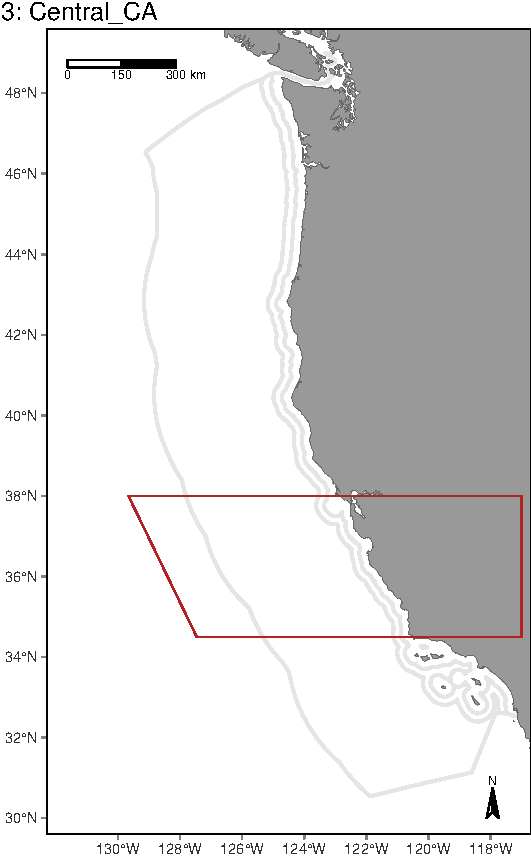
\includegraphics{figures/unnamed-chunk-56-3.pdf} 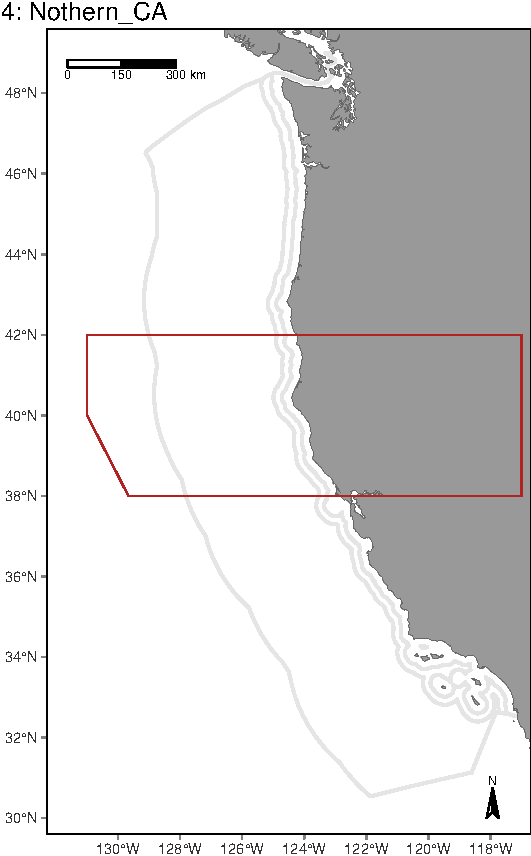
\includegraphics{figures/unnamed-chunk-56-4.pdf} 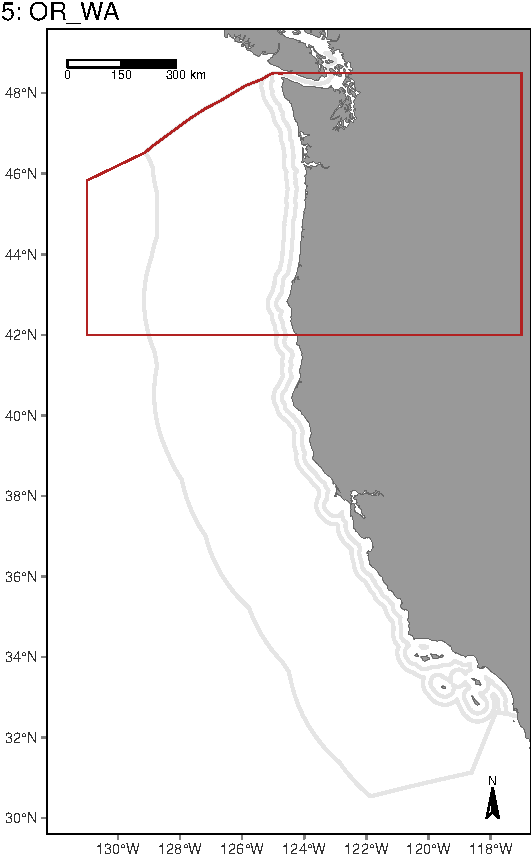
\includegraphics{figures/unnamed-chunk-56-5.pdf}

\hypertarget{etp}{%
\section*{ETP}\label{etp}}
\addcontentsline{toc}{section}{ETP}

\begin{Shaded}
\begin{Highlighting}[]
\KeywordTok{strata_explore}\NormalTok{(}\StringTok{'etp'}\NormalTok{)}
\end{Highlighting}
\end{Shaded}

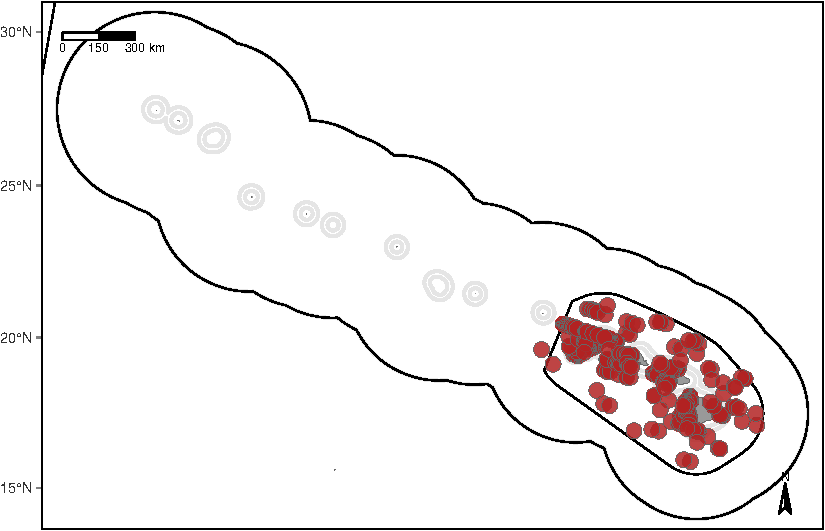
\includegraphics{figures/unnamed-chunk-57-1.pdf} 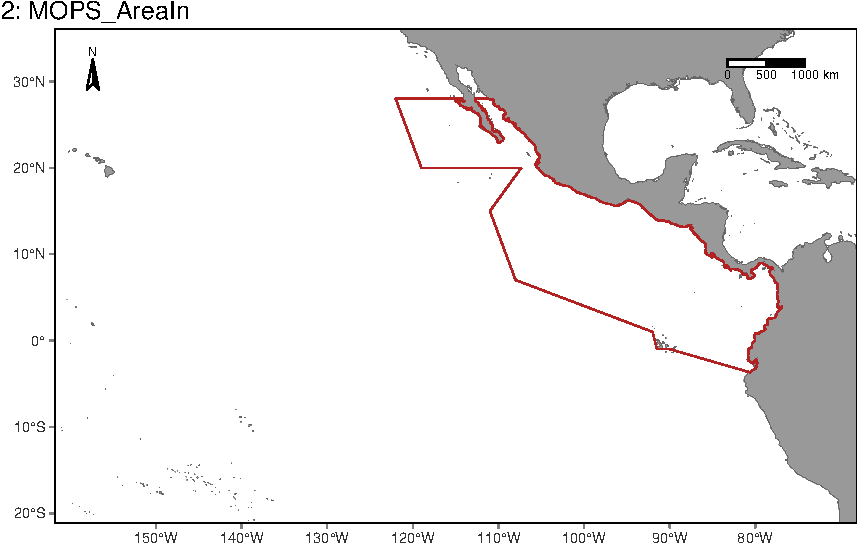
\includegraphics{figures/unnamed-chunk-57-2.pdf} 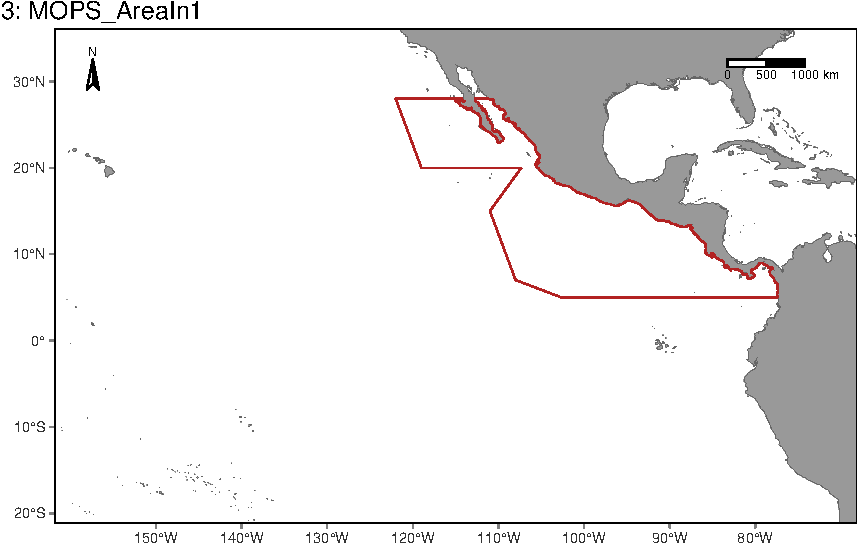
\includegraphics{figures/unnamed-chunk-57-3.pdf} 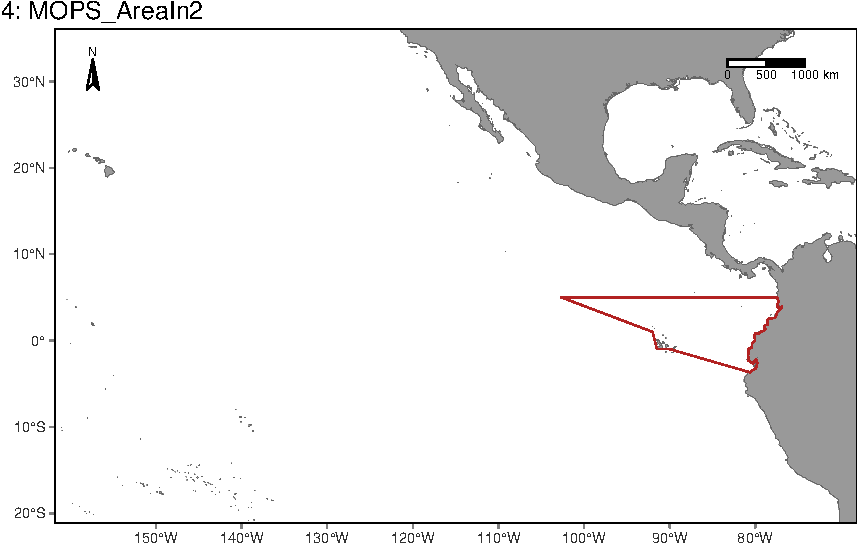
\includegraphics{figures/unnamed-chunk-57-4.pdf} 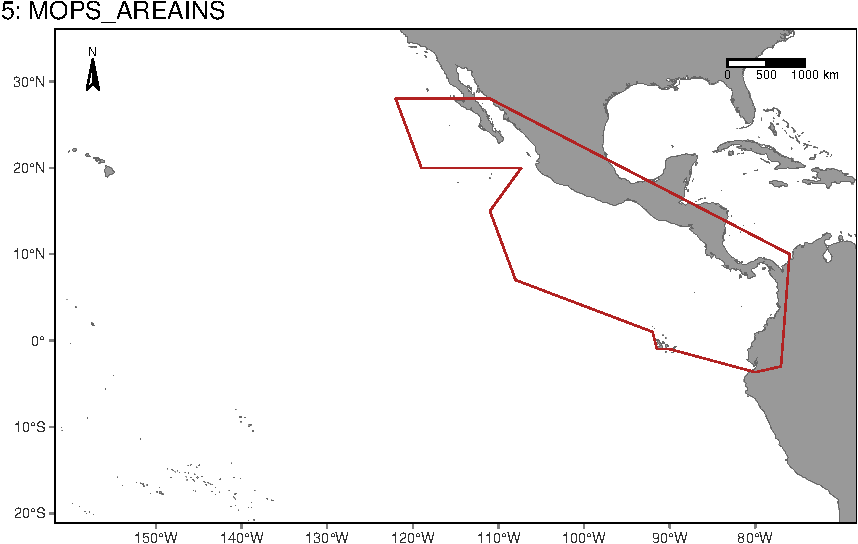
\includegraphics{figures/unnamed-chunk-57-5.pdf} 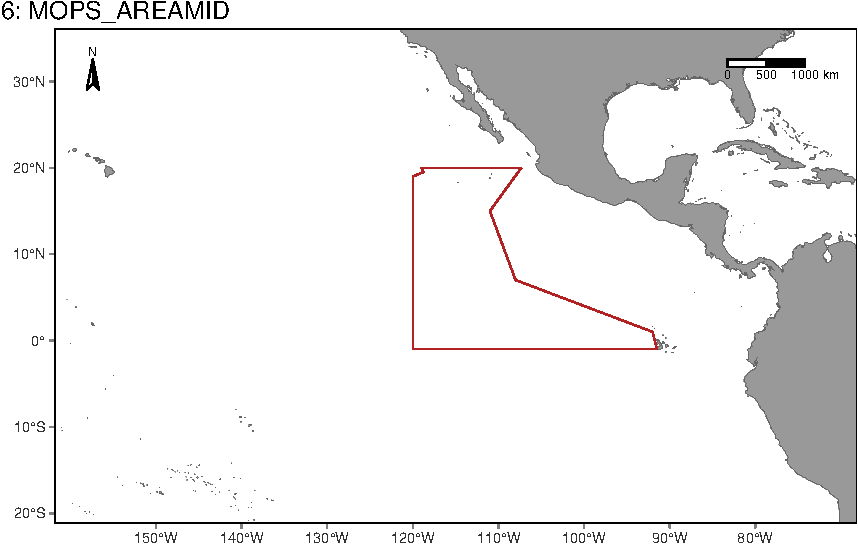
\includegraphics{figures/unnamed-chunk-57-6.pdf} 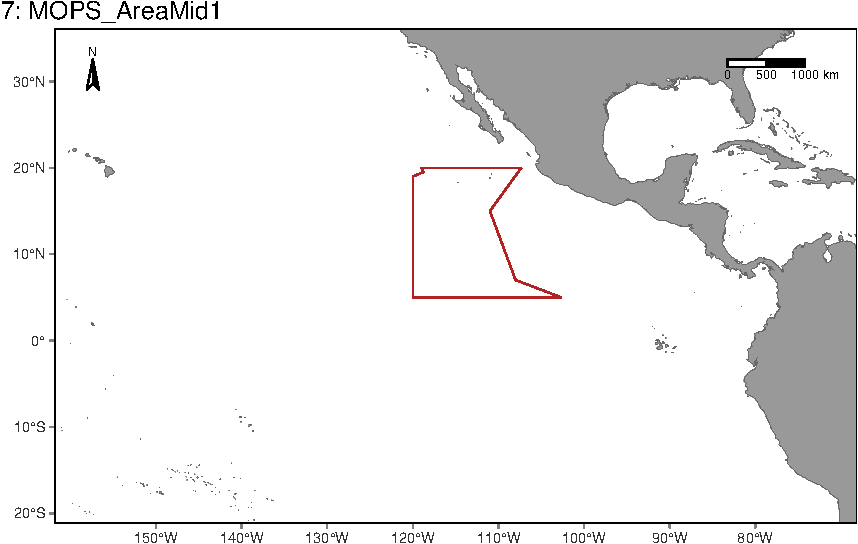
\includegraphics{figures/unnamed-chunk-57-7.pdf} 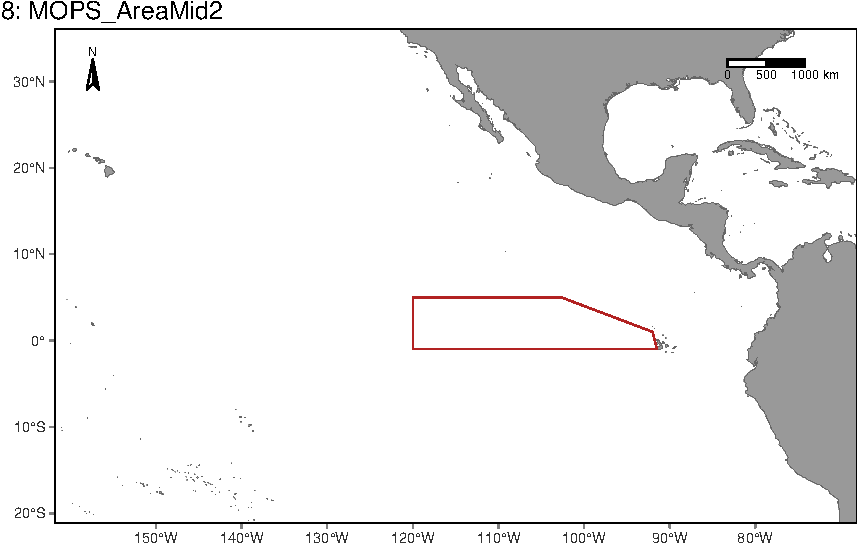
\includegraphics{figures/unnamed-chunk-57-8.pdf} 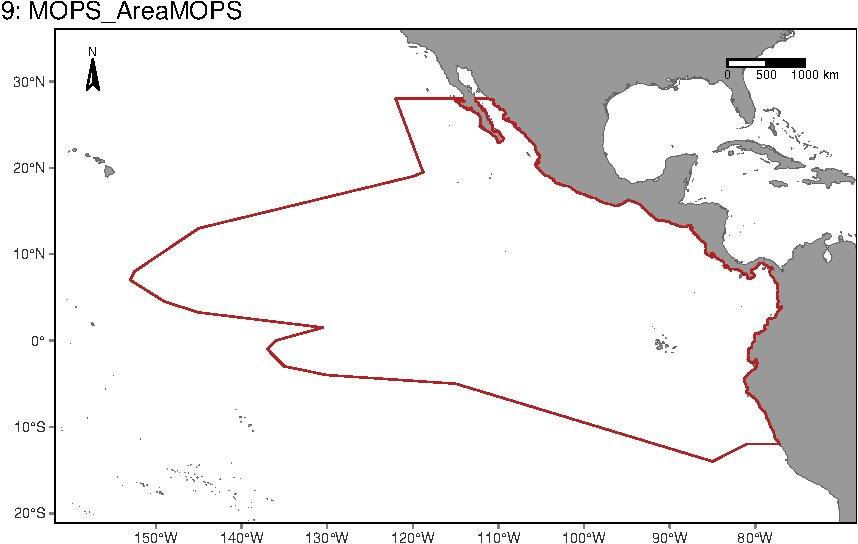
\includegraphics{figures/unnamed-chunk-57-9.pdf} 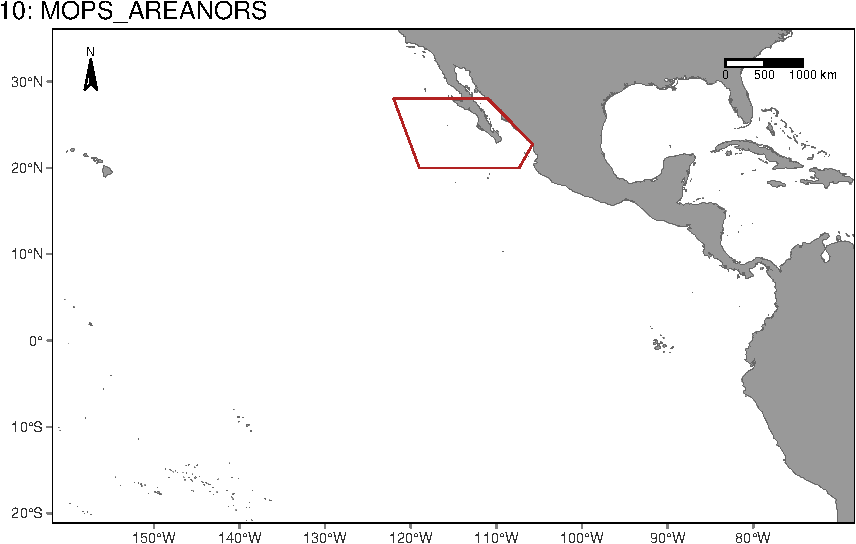
\includegraphics{figures/unnamed-chunk-57-10.pdf} 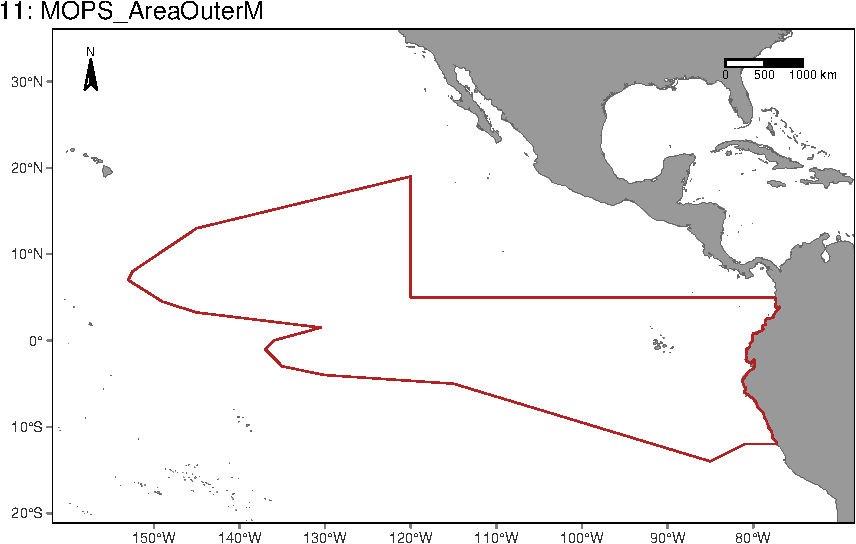
\includegraphics{figures/unnamed-chunk-57-11.pdf} 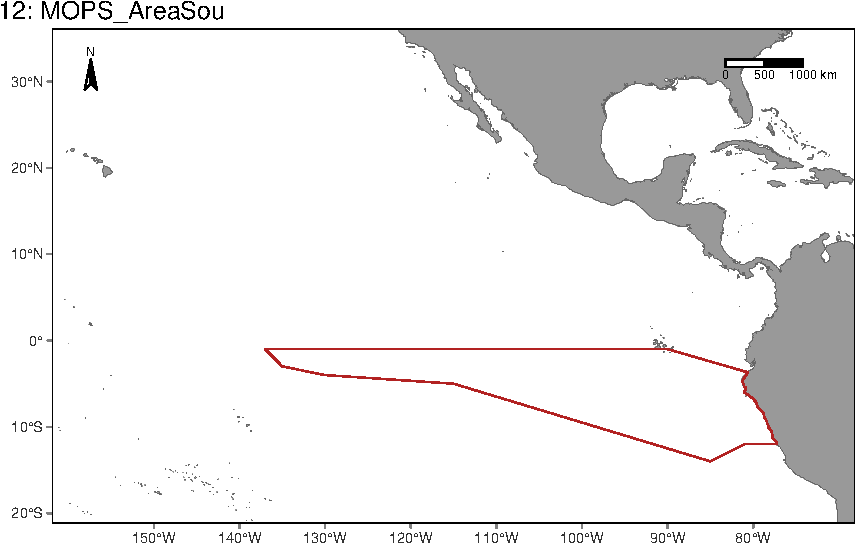
\includegraphics{figures/unnamed-chunk-57-12.pdf} 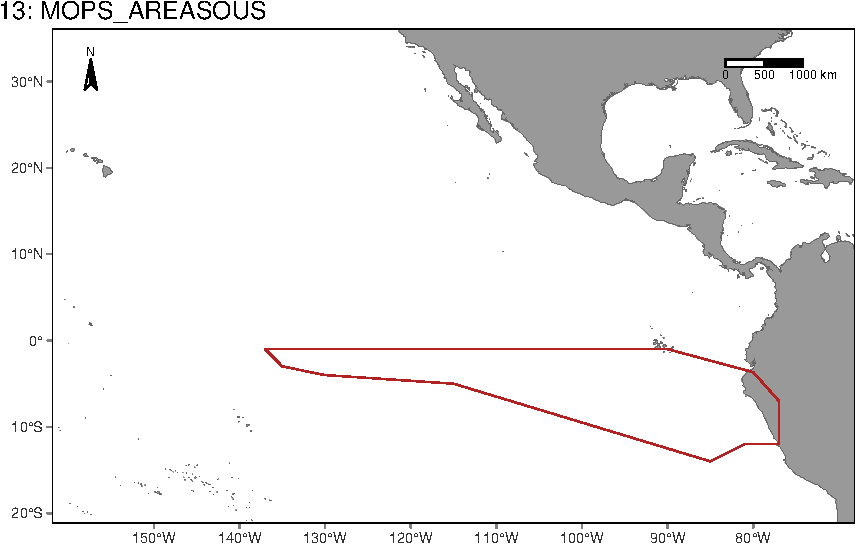
\includegraphics{figures/unnamed-chunk-57-13.pdf} 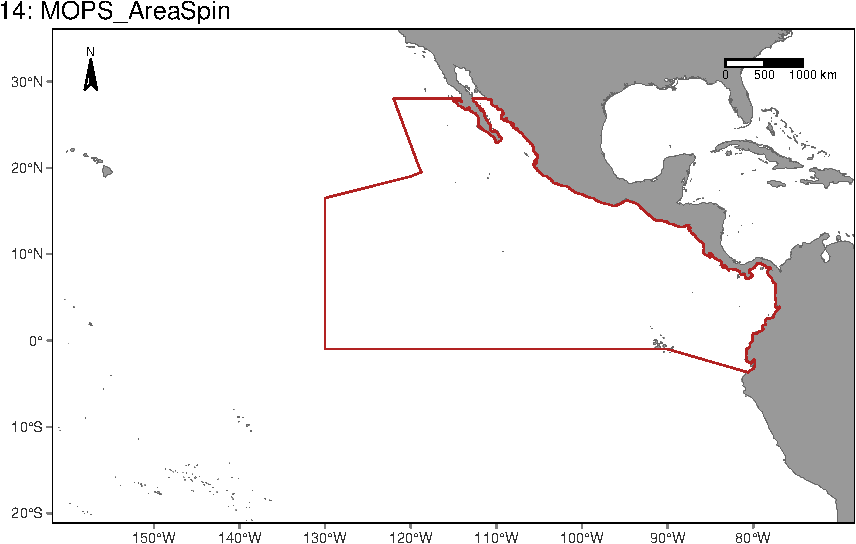
\includegraphics{figures/unnamed-chunk-57-14.pdf} 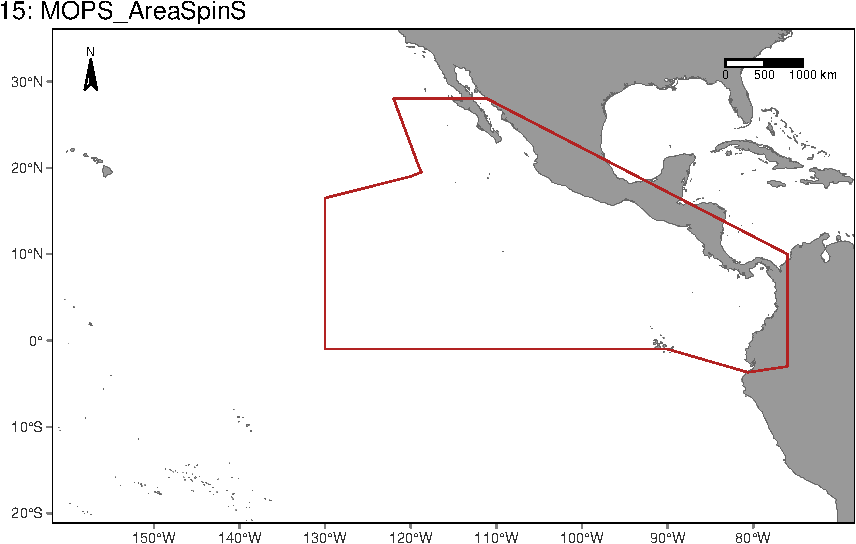
\includegraphics{figures/unnamed-chunk-57-15.pdf} 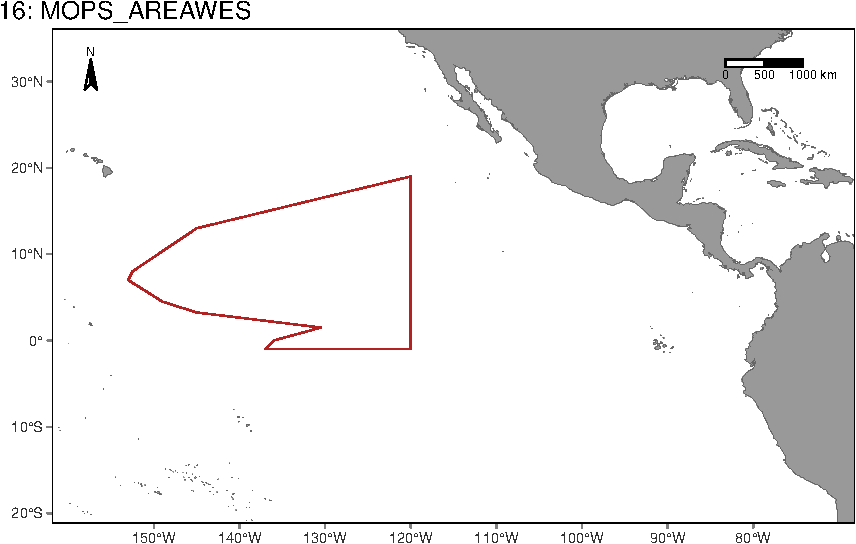
\includegraphics{figures/unnamed-chunk-57-16.pdf} 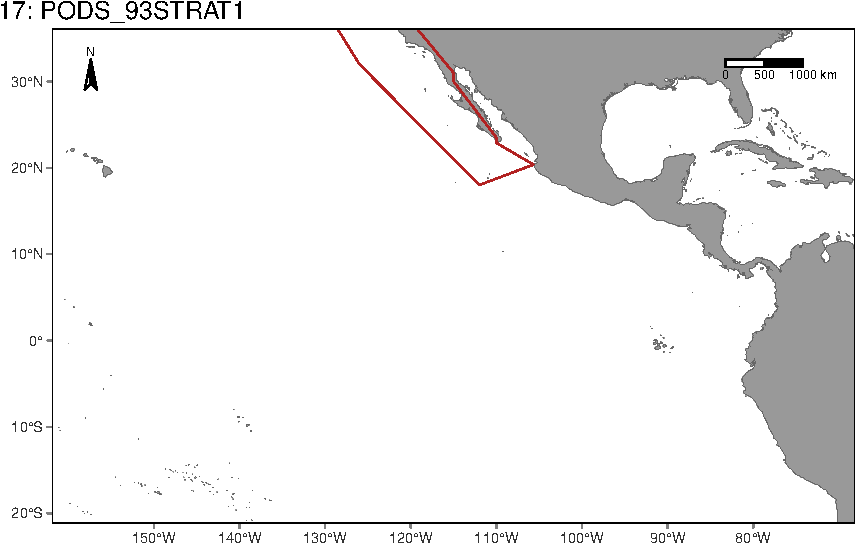
\includegraphics{figures/unnamed-chunk-57-17.pdf} 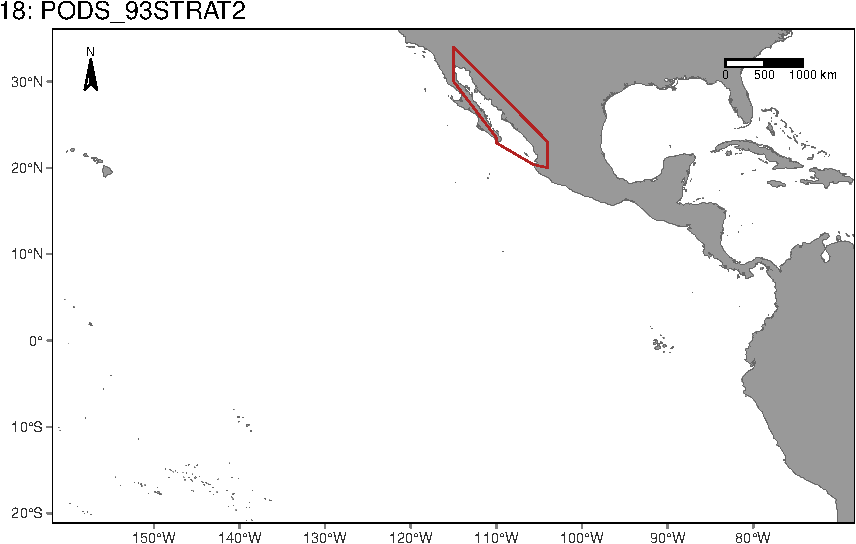
\includegraphics{figures/unnamed-chunk-57-18.pdf} 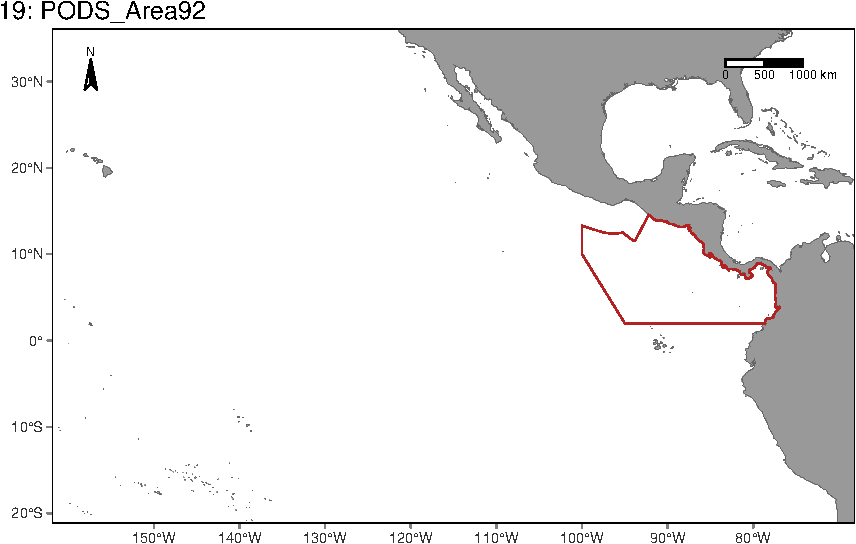
\includegraphics{figures/unnamed-chunk-57-19.pdf} 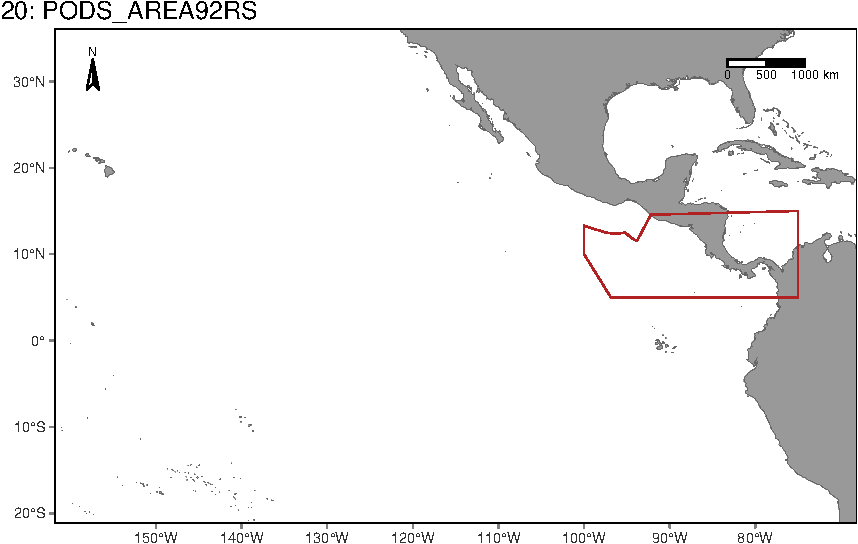
\includegraphics{figures/unnamed-chunk-57-20.pdf} 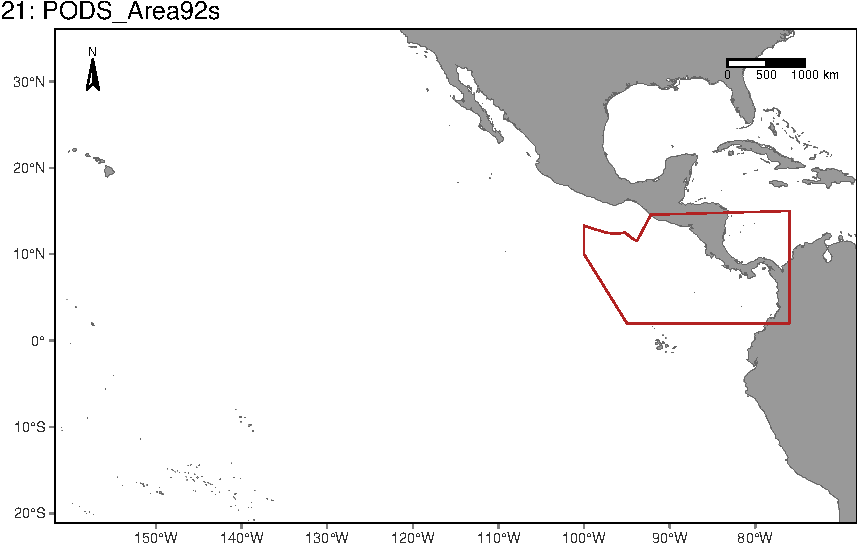
\includegraphics{figures/unnamed-chunk-57-21.pdf} 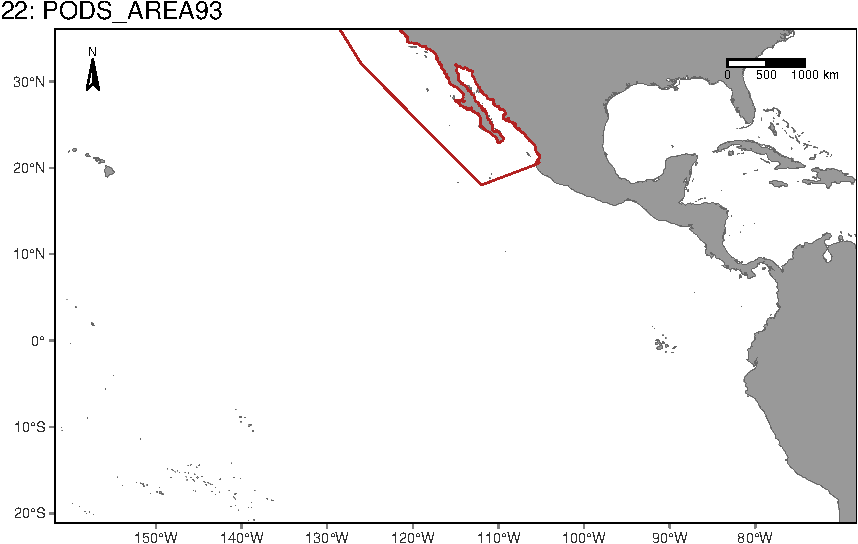
\includegraphics{figures/unnamed-chunk-57-22.pdf} 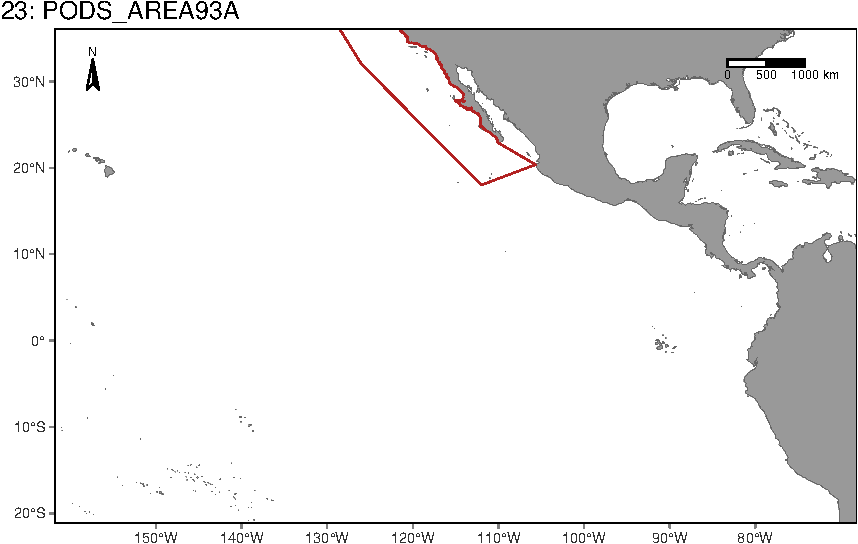
\includegraphics{figures/unnamed-chunk-57-23.pdf} 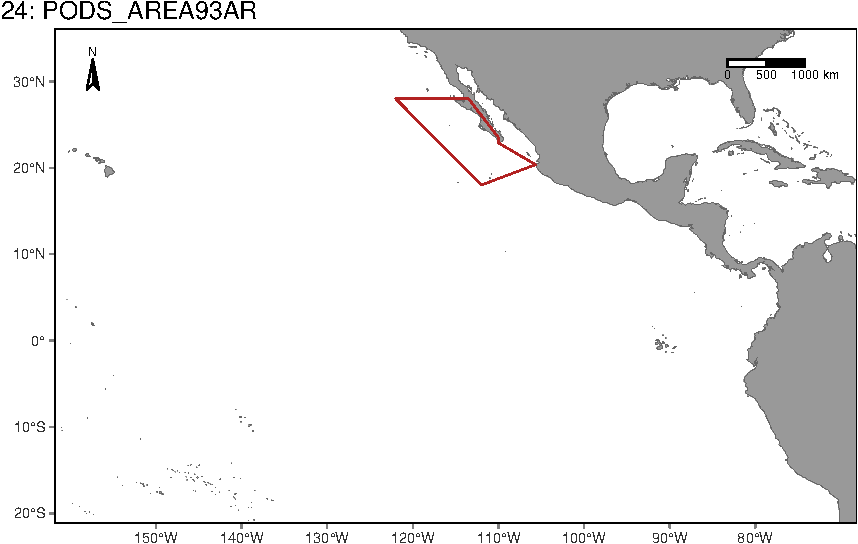
\includegraphics{figures/unnamed-chunk-57-24.pdf} 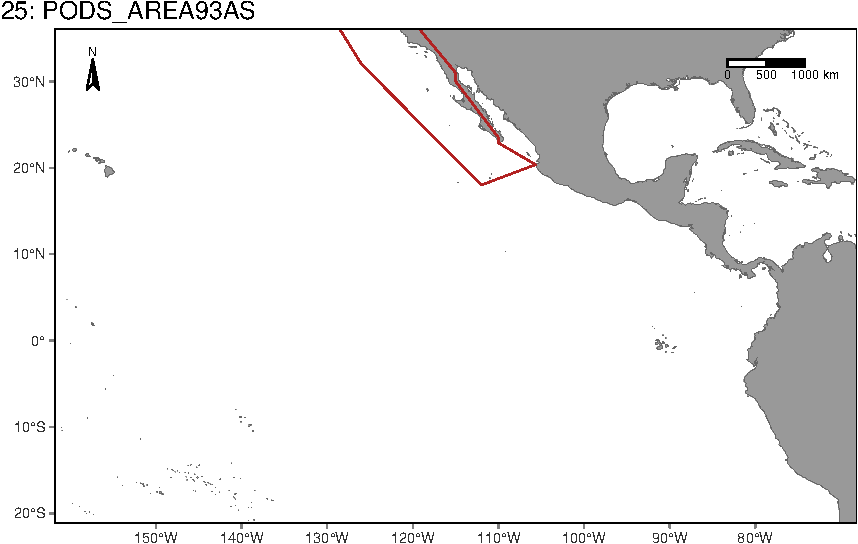
\includegraphics{figures/unnamed-chunk-57-25.pdf} 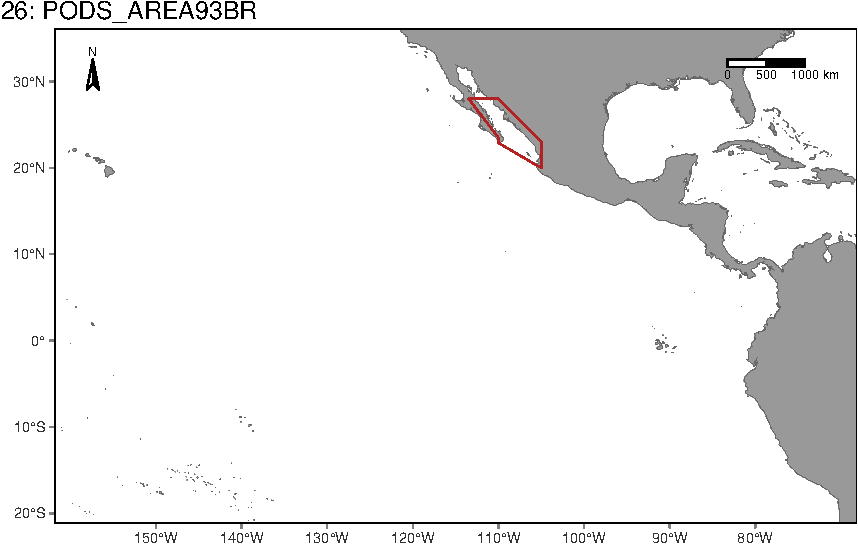
\includegraphics{figures/unnamed-chunk-57-26.pdf} 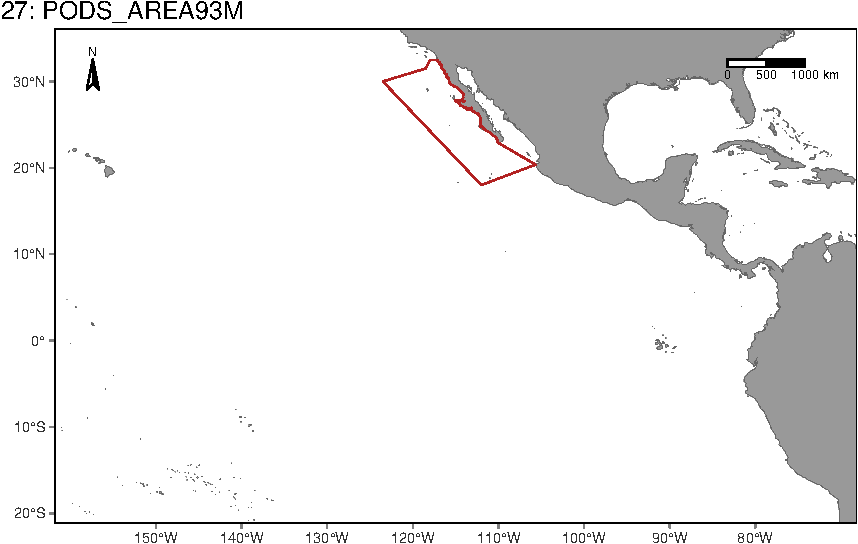
\includegraphics{figures/unnamed-chunk-57-27.pdf} 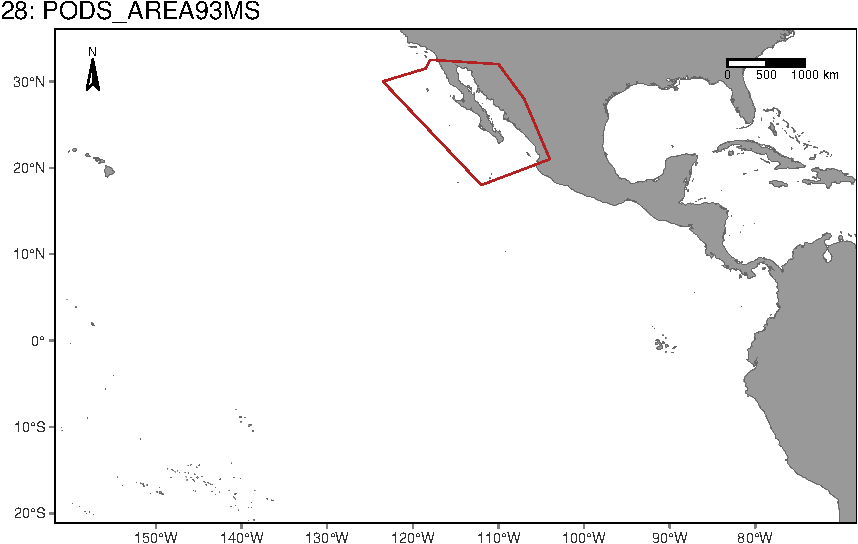
\includegraphics{figures/unnamed-chunk-57-28.pdf} 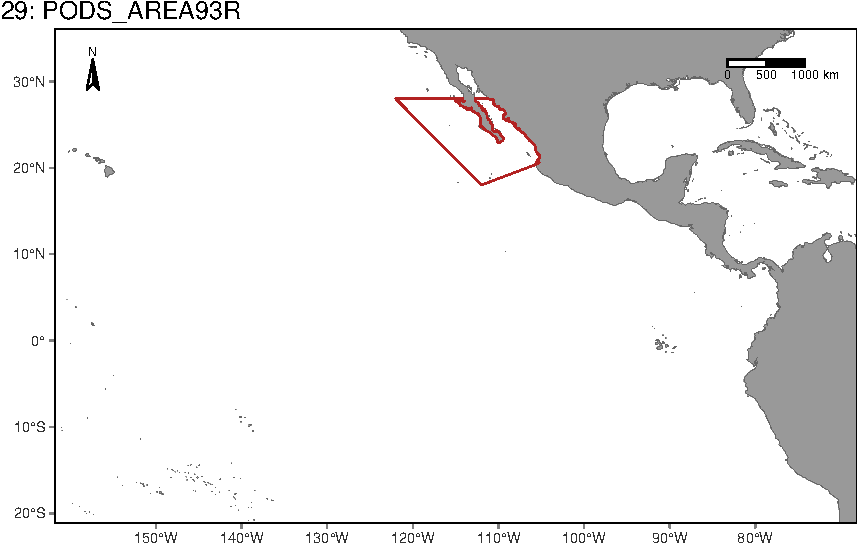
\includegraphics{figures/unnamed-chunk-57-29.pdf} 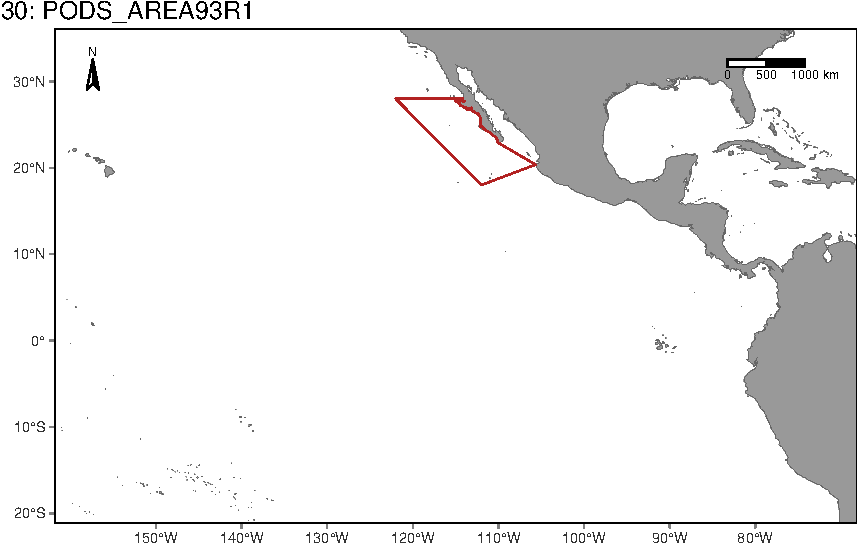
\includegraphics{figures/unnamed-chunk-57-30.pdf} 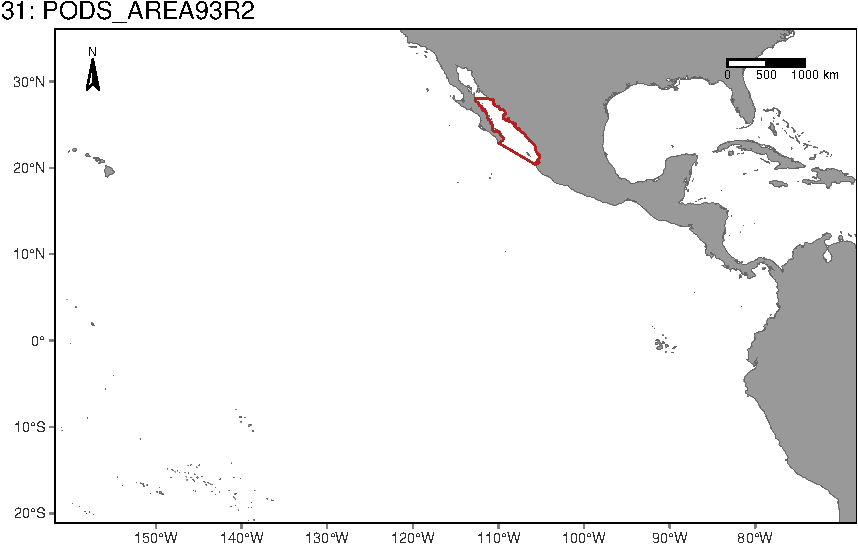
\includegraphics{figures/unnamed-chunk-57-31.pdf} 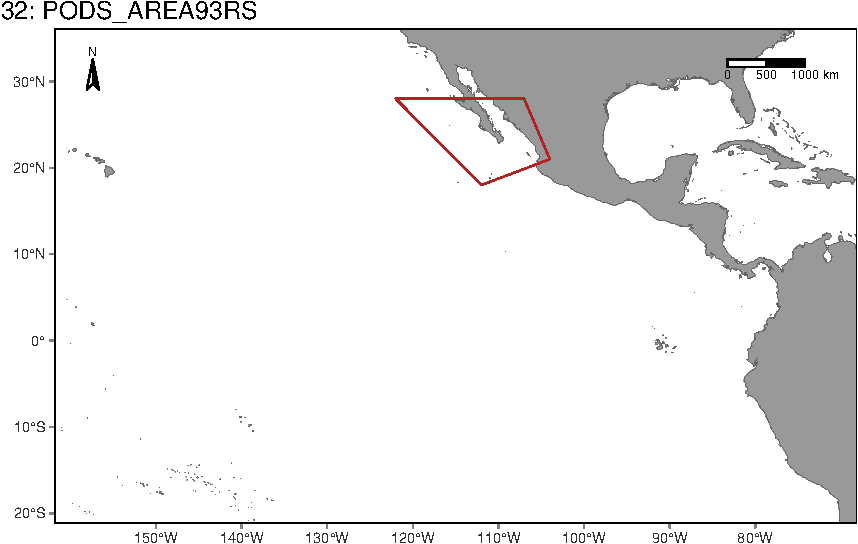
\includegraphics{figures/unnamed-chunk-57-32.pdf} 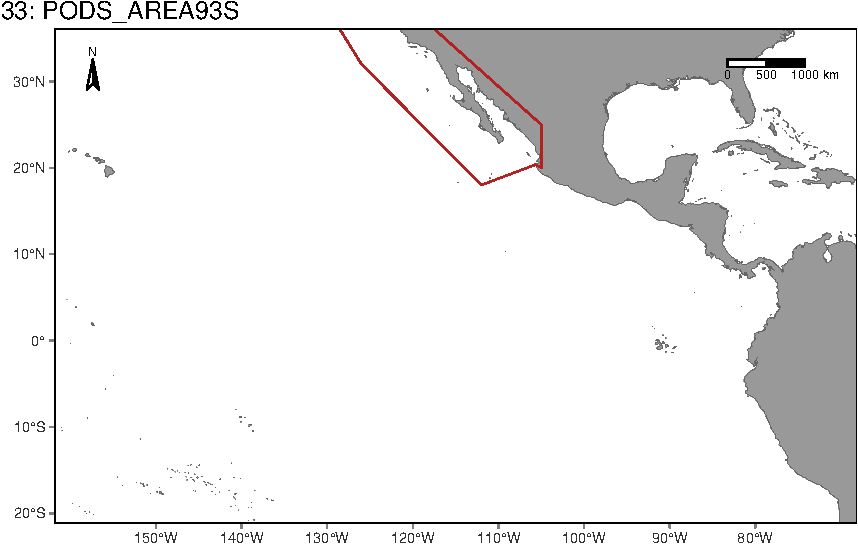
\includegraphics{figures/unnamed-chunk-57-33.pdf} \includegraphics{figures/unnamed-chunk-57-34.pdf} \includegraphics{figures/unnamed-chunk-57-35.pdf} \includegraphics{figures/unnamed-chunk-57-36.pdf} \includegraphics{figures/unnamed-chunk-57-37.pdf} \includegraphics{figures/unnamed-chunk-57-38.pdf} \includegraphics{figures/unnamed-chunk-57-39.pdf} \includegraphics{figures/unnamed-chunk-57-40.pdf} \includegraphics{figures/unnamed-chunk-57-41.pdf} \includegraphics{figures/unnamed-chunk-57-42.pdf} \includegraphics{figures/unnamed-chunk-57-43.pdf} \includegraphics{figures/unnamed-chunk-57-44.pdf} \includegraphics{figures/unnamed-chunk-57-45.pdf} \includegraphics{figures/unnamed-chunk-57-46.pdf} \includegraphics{figures/unnamed-chunk-57-47.pdf} \includegraphics{figures/unnamed-chunk-57-48.pdf} \includegraphics{figures/unnamed-chunk-57-49.pdf} \includegraphics{figures/unnamed-chunk-57-50.pdf} \includegraphics{figures/unnamed-chunk-57-51.pdf} \includegraphics{figures/unnamed-chunk-57-52.pdf} \includegraphics{figures/unnamed-chunk-57-53.pdf} \includegraphics{figures/unnamed-chunk-57-54.pdf} \includegraphics{figures/unnamed-chunk-57-55.pdf} \includegraphics{figures/unnamed-chunk-57-56.pdf} \includegraphics{figures/unnamed-chunk-57-57.pdf} \includegraphics{figures/unnamed-chunk-57-58.pdf} \includegraphics{figures/unnamed-chunk-57-59.pdf} \includegraphics{figures/unnamed-chunk-57-60.pdf} \includegraphics{figures/unnamed-chunk-57-61.pdf} \includegraphics{figures/unnamed-chunk-57-62.pdf} \includegraphics{figures/unnamed-chunk-57-63.pdf} \includegraphics{figures/unnamed-chunk-57-64.pdf} \includegraphics{figures/unnamed-chunk-57-65.pdf} \includegraphics{figures/unnamed-chunk-57-66.pdf} \includegraphics{figures/unnamed-chunk-57-67.pdf} \includegraphics{figures/unnamed-chunk-57-68.pdf} \includegraphics{figures/unnamed-chunk-57-69.pdf} \includegraphics{figures/unnamed-chunk-57-70.pdf}

\hypertarget{segmentizing}{%
\chapter{Appendix: Segmentizing}\label{segmentizing}}

The package's \texttt{segmentize()} function and its associated settings were designed to give researchers full control over how data are segmented, be it for design-based density analysis (which tend to use long segments of 100 km or more and allow for non-contiguous effort to be included in the same segment) or for habitat modeling (which tend to use short segments of 5 - 10 km and disallow non-contiguous effort to be pooled into the same segment).

The demonstration of \texttt{segmentize()} on in \protect\hyperlink{processing}{Processing chapter} relies on the \texttt{settings} object that is attached as a slot in the \texttt{cruz} object. But you can override those settings with direct function inputs in \texttt{segmentize()}, which gives us a chance to explore segmentization options.

First we loadthe demo data and carry out initial processing:

\begin{Shaded}
\begin{Highlighting}[]
\KeywordTok{data}\NormalTok{(settings)}
\NormalTok{das_file <-}\StringTok{ 'data/surveys/HICEASwinter2020.das'}
\NormalTok{das <-}\StringTok{ }\KeywordTok{load_das}\NormalTok{(das_file, }
                \DataTypeTok{perform_checks =} \OtherTok{FALSE}\NormalTok{,}
                \DataTypeTok{print_glimpse =} \OtherTok{FALSE}\NormalTok{)}
\NormalTok{das <-}\StringTok{ }\KeywordTok{format_das}\NormalTok{(das, settings)}
\NormalTok{cruz <-}\StringTok{ }\KeywordTok{process_strata}\NormalTok{(das,}
\NormalTok{                       settings,}
                       \DataTypeTok{verbose=}\OtherTok{FALSE}\NormalTok{)}
\end{Highlighting}
\end{Shaded}

And this is the histogram function we will be using to display the results of each run of \texttt{segmentize()}:

\begin{Shaded}
\begin{Highlighting}[]
\NormalTok{segment_histogram <-}\StringTok{ }\ControlFlowTok{function}\NormalTok{(cohort_effort, }\DataTypeTok{by_day=}\OtherTok{FALSE}\NormalTok{)\{}
\NormalTok{  segs <-}\StringTok{ }\NormalTok{cohort_effort}\OperatorTok{$}\NormalTok{segments}
\NormalTok{  segmax <-}\StringTok{ }\KeywordTok{max}\NormalTok{(segs}\OperatorTok{$}\NormalTok{dist,}\DataTypeTok{na.rm=}\OtherTok{TRUE}\NormalTok{)}\OperatorTok{*}\FloatTok{1.1}
  
  \ControlFlowTok{if}\NormalTok{(by_day)\{}
\NormalTok{    main_use <-}\StringTok{ }\KeywordTok{paste0}\NormalTok{(}\StringTok{'Segments (use) |  by day'}\NormalTok{)}
\NormalTok{    main_exclude <-}\StringTok{ }\KeywordTok{paste0}\NormalTok{(}\StringTok{'Segments (exclude) |  by day'}\NormalTok{)}
\NormalTok{  \}}\ControlFlowTok{else}\NormalTok{\{}
\NormalTok{    main_use <-}\StringTok{ }\KeywordTok{paste0}\NormalTok{(}\StringTok{'Segments (use) |  target: '}\NormalTok{,settings}\OperatorTok{$}\NormalTok{survey}\OperatorTok{$}\NormalTok{segment_target_km,}\StringTok{' km'}\NormalTok{)}
\NormalTok{    main_exclude <-}\StringTok{ }\KeywordTok{paste0}\NormalTok{(}\StringTok{'Segments (exclude) |  target: '}\NormalTok{,settings}\OperatorTok{$}\NormalTok{survey}\OperatorTok{$}\NormalTok{segment_target_km,}\StringTok{' km'}\NormalTok{)}
\NormalTok{  \}}
  \KeywordTok{par}\NormalTok{(}\DataTypeTok{mfrow=}\KeywordTok{c}\NormalTok{(}\DecValTok{1}\NormalTok{,}\DecValTok{2}\NormalTok{))}
  \KeywordTok{par}\NormalTok{(}\DataTypeTok{mar=}\KeywordTok{c}\NormalTok{(}\FloatTok{4.2}\NormalTok{,}\FloatTok{4.2}\NormalTok{,}\FloatTok{2.5}\NormalTok{,.}\DecValTok{5}\NormalTok{))}
  \KeywordTok{hist}\NormalTok{(segs}\OperatorTok{$}\NormalTok{dist[segs}\OperatorTok{$}\NormalTok{use],}
       \DataTypeTok{breaks =} \KeywordTok{seq}\NormalTok{(}\DecValTok{0}\NormalTok{,segmax,}\DataTypeTok{by=}\NormalTok{segmax}\OperatorTok{/}\DecValTok{40}\NormalTok{),}
       \DataTypeTok{xlab=}\StringTok{'Segment lengths (km)'}\NormalTok{,}
       \DataTypeTok{main=}\NormalTok{main_use,}
       \DataTypeTok{cex.main =} \FloatTok{.8}\NormalTok{, }\DataTypeTok{cex.axis =} \FloatTok{.8}\NormalTok{, }\DataTypeTok{cex.lab =} \FloatTok{.8}\NormalTok{)}

  \KeywordTok{hist}\NormalTok{(segs}\OperatorTok{$}\NormalTok{dist[}\OperatorTok{!}\NormalTok{segs}\OperatorTok{$}\NormalTok{use],}
       \DataTypeTok{breaks =} \KeywordTok{seq}\NormalTok{(}\DecValTok{0}\NormalTok{,segmax,}\DataTypeTok{by=}\NormalTok{segmax}\OperatorTok{/}\DecValTok{40}\NormalTok{),}
       \DataTypeTok{xlab=}\StringTok{'Segment lengths (km)'}\NormalTok{,}
       \DataTypeTok{main=}\NormalTok{main_exclude,}
       \DataTypeTok{cex.main =} \FloatTok{.8}\NormalTok{, }\DataTypeTok{cex.axis =} \FloatTok{.8}\NormalTok{, }\DataTypeTok{cex.lab =} \FloatTok{.8}\NormalTok{)}
  \KeywordTok{par}\NormalTok{(}\DataTypeTok{mfrow=}\KeywordTok{c}\NormalTok{(}\DecValTok{1}\NormalTok{,}\DecValTok{1}\NormalTok{))}
\NormalTok{\}}
\end{Highlighting}
\end{Shaded}

\hypertarget{defaults-2}{%
\section*{Defaults}\label{defaults-2}}
\addcontentsline{toc}{section}{Defaults}

Here is the \texttt{segmentize()} function parameterized with the ``factory default'' settings from \texttt{load\_settings()}.

\begin{Shaded}
\begin{Highlighting}[]
\NormalTok{cruz_demo <-}\StringTok{ }\KeywordTok{segmentize}\NormalTok{(cruz,}
                        \DataTypeTok{segment_method =} \StringTok{'equallength'}\NormalTok{,}
                        \DataTypeTok{segment_target_km =} \DecValTok{30}\NormalTok{,}
                        \DataTypeTok{segment_max_interval =} \DecValTok{48}\NormalTok{,}
                        \DataTypeTok{segment_type_handling =} \StringTok{'separate'}\NormalTok{,}
                        \DataTypeTok{segment_remainder_handling =} \KeywordTok{c}\NormalTok{(}\StringTok{'append'}\NormalTok{,}\StringTok{'segment'}\NormalTok{),}
                        \DataTypeTok{density_types =} \KeywordTok{c}\NormalTok{(}\StringTok{'S'}\NormalTok{,}\StringTok{'F'}\NormalTok{),}
                        \DataTypeTok{density_modes =} \KeywordTok{c}\NormalTok{(}\StringTok{'P'}\NormalTok{,}\StringTok{'C'}\NormalTok{),}
                        \DataTypeTok{density_on_off =} \KeywordTok{c}\NormalTok{(}\OtherTok{TRUE}\NormalTok{),}
                        \DataTypeTok{distance_types =} \OtherTok{NULL}\NormalTok{,}
                        \DataTypeTok{distance_modes =} \OtherTok{NULL}\NormalTok{,}
                        \DataTypeTok{distance_on_off =} \OtherTok{NULL}\NormalTok{,}
                        \DataTypeTok{random_seed =} \OtherTok{NULL}\NormalTok{)}
\NormalTok{[}\DecValTok{1}\NormalTok{] }\StringTok{"separate"}
\NormalTok{[}\DecValTok{1}\NormalTok{] }\StringTok{"append"}  \StringTok{"segment"}
\NormalTok{[}\DecValTok{1}\NormalTok{] }\StringTok{"equallength"}
\NormalTok{[}\DecValTok{1}\NormalTok{] }\DecValTok{833171}
\NormalTok{[}\DecValTok{1}\NormalTok{] }\DecValTok{172800}
\NormalTok{[}\DecValTok{1}\NormalTok{] }\DecValTok{30}
\NormalTok{[}\DecValTok{1}\NormalTok{] }\StringTok{"S"} \StringTok{"F"}
\NormalTok{[}\DecValTok{1}\NormalTok{] }\StringTok{"P"} \StringTok{"C"}
\NormalTok{[}\DecValTok{1}\NormalTok{] }\OtherTok{TRUE}
\NormalTok{[}\DecValTok{1}\NormalTok{] }\StringTok{"S"} \StringTok{"F"}
\NormalTok{[}\DecValTok{1}\NormalTok{] }\StringTok{"P"} \StringTok{"C"}
\NormalTok{[}\DecValTok{1}\NormalTok{] }\OtherTok{TRUE}
\NormalTok{[}\DecValTok{1}\NormalTok{] }\StringTok{"separate"}
\NormalTok{[}\DecValTok{1}\NormalTok{] }\StringTok{"append"}  \StringTok{"segment"}
\NormalTok{[}\DecValTok{1}\NormalTok{] }\StringTok{"equallength"}
\NormalTok{[}\DecValTok{1}\NormalTok{] }\DecValTok{833171}
\NormalTok{[}\DecValTok{1}\NormalTok{] }\DecValTok{172800}
\NormalTok{[}\DecValTok{1}\NormalTok{] }\DecValTok{30}
\NormalTok{[}\DecValTok{1}\NormalTok{] }\StringTok{"S"} \StringTok{"F"}
\NormalTok{[}\DecValTok{1}\NormalTok{] }\StringTok{"P"} \StringTok{"C"}
\NormalTok{[}\DecValTok{1}\NormalTok{] }\OtherTok{TRUE}
\NormalTok{[}\DecValTok{1}\NormalTok{] }\StringTok{"S"} \StringTok{"F"} \StringTok{"N"}
\NormalTok{[}\DecValTok{1}\NormalTok{] }\StringTok{"P"} \StringTok{"C"}
\NormalTok{[}\DecValTok{1}\NormalTok{] }\OtherTok{TRUE}

\CommentTok{# Number of segments}
\NormalTok{cruz_demo}\OperatorTok{$}\NormalTok{cohorts}\OperatorTok{$}\NormalTok{default}\OperatorTok{$}\NormalTok{density}\OperatorTok{$}\NormalTok{segments }\OperatorTok\StringTok{ }\NormalTok{nrow}
\NormalTok{[}\DecValTok{1}\NormalTok{] }\DecValTok{278}

\CommentTok{# Plot}
\KeywordTok{segment_histogram}\NormalTok{(cruz_demo}\OperatorTok{$}\NormalTok{cohorts}\OperatorTok{$}\NormalTok{default}\OperatorTok{$}\NormalTok{density)}
\end{Highlighting}
\end{Shaded}

\includegraphics{figures/unnamed-chunk-61-1.pdf}

\hypertarget{day-vs-equal-length}{%
\section*{Day vs Equal Length}\label{day-vs-equal-length}}
\addcontentsline{toc}{section}{Day vs Equal Length}

\begin{Shaded}
\begin{Highlighting}[]
\NormalTok{cruz_demo <-}\StringTok{ }\KeywordTok{segmentize}\NormalTok{(cruz,}
                        \DataTypeTok{segment_method =} \StringTok{'day'}\NormalTok{,}
                        \DataTypeTok{segment_target_km =} \DecValTok{30}\NormalTok{,}
                        \DataTypeTok{segment_max_interval =} \DecValTok{48}\NormalTok{,}
                        \DataTypeTok{segment_type_handling =} \StringTok{'separate'}\NormalTok{,}
                        \DataTypeTok{segment_remainder_handling =} \KeywordTok{c}\NormalTok{(}\StringTok{'append'}\NormalTok{,}\StringTok{'segment'}\NormalTok{),}
                        \DataTypeTok{density_types =} \KeywordTok{c}\NormalTok{(}\StringTok{'S'}\NormalTok{,}\StringTok{'F'}\NormalTok{),}
                        \DataTypeTok{density_modes =} \KeywordTok{c}\NormalTok{(}\StringTok{'P'}\NormalTok{,}\StringTok{'C'}\NormalTok{),}
                        \DataTypeTok{density_on_off =} \KeywordTok{c}\NormalTok{(}\OtherTok{TRUE}\NormalTok{),}
                        \DataTypeTok{distance_types =} \OtherTok{NULL}\NormalTok{,}
                        \DataTypeTok{distance_modes =} \OtherTok{NULL}\NormalTok{,}
                        \DataTypeTok{distance_on_off =} \OtherTok{NULL}\NormalTok{,}
                        \DataTypeTok{random_seed =} \OtherTok{NULL}\NormalTok{)}
\NormalTok{[}\DecValTok{1}\NormalTok{] }\StringTok{"separate"}
\NormalTok{[}\DecValTok{1}\NormalTok{] }\StringTok{"append"}  \StringTok{"segment"}
\NormalTok{[}\DecValTok{1}\NormalTok{] }\StringTok{"day"}
\NormalTok{[}\DecValTok{1}\NormalTok{] }\DecValTok{833171}
\NormalTok{[}\DecValTok{1}\NormalTok{] }\DecValTok{172800}
\NormalTok{[}\DecValTok{1}\NormalTok{] }\DecValTok{30}
\NormalTok{[}\DecValTok{1}\NormalTok{] }\StringTok{"S"} \StringTok{"F"}
\NormalTok{[}\DecValTok{1}\NormalTok{] }\StringTok{"P"} \StringTok{"C"}
\NormalTok{[}\DecValTok{1}\NormalTok{] }\OtherTok{TRUE}
\NormalTok{[}\DecValTok{1}\NormalTok{] }\StringTok{"S"} \StringTok{"F"}
\NormalTok{[}\DecValTok{1}\NormalTok{] }\StringTok{"P"} \StringTok{"C"}
\NormalTok{[}\DecValTok{1}\NormalTok{] }\OtherTok{TRUE}
\NormalTok{[}\DecValTok{1}\NormalTok{] }\StringTok{"separate"}
\NormalTok{[}\DecValTok{1}\NormalTok{] }\StringTok{"append"}  \StringTok{"segment"}
\NormalTok{[}\DecValTok{1}\NormalTok{] }\StringTok{"day"}
\NormalTok{[}\DecValTok{1}\NormalTok{] }\DecValTok{833171}
\NormalTok{[}\DecValTok{1}\NormalTok{] }\DecValTok{172800}
\NormalTok{[}\DecValTok{1}\NormalTok{] }\DecValTok{30}
\NormalTok{[}\DecValTok{1}\NormalTok{] }\StringTok{"S"} \StringTok{"F"}
\NormalTok{[}\DecValTok{1}\NormalTok{] }\StringTok{"P"} \StringTok{"C"}
\NormalTok{[}\DecValTok{1}\NormalTok{] }\OtherTok{TRUE}
\NormalTok{[}\DecValTok{1}\NormalTok{] }\StringTok{"S"} \StringTok{"F"} \StringTok{"N"}
\NormalTok{[}\DecValTok{1}\NormalTok{] }\StringTok{"P"} \StringTok{"C"}
\NormalTok{[}\DecValTok{1}\NormalTok{] }\OtherTok{TRUE}

\CommentTok{# Number of segments}
\NormalTok{cruz_demo}\OperatorTok{$}\NormalTok{cohorts}\OperatorTok{$}\NormalTok{default}\OperatorTok{$}\NormalTok{density}\OperatorTok{$}\NormalTok{segments }\OperatorTok\StringTok{ }\NormalTok{nrow}
\NormalTok{[}\DecValTok{1}\NormalTok{] }\DecValTok{96}

\CommentTok{# Plot}
\KeywordTok{segment_histogram}\NormalTok{(cruz_demo}\OperatorTok{$}\NormalTok{cohorts}\OperatorTok{$}\NormalTok{default}\OperatorTok{$}\NormalTok{density, }\DataTypeTok{by_day =} \OtherTok{TRUE}\NormalTok{)}
\end{Highlighting}
\end{Shaded}

\includegraphics{figures/unnamed-chunk-63-1.pdf}

\hypertarget{contiguous-vs.-non-contiguous-effort}{%
\section*{Contiguous vs.~non-contiguous effort}\label{contiguous-vs.-non-contiguous-effort}}
\addcontentsline{toc}{section}{Contiguous vs.~non-contiguous effort}

The example above allows for non-contiguous effort; a segment is allowed to contain effort separated by gaps as large as 24 hours (\texttt{settings\$max\_interval}). To coerce segments to represent only contiguous effort, make that setting very small:

\begin{Shaded}
\begin{Highlighting}[]
\NormalTok{cruz_demo <-}\StringTok{ }\KeywordTok{segmentize}\NormalTok{(cruz,}
                        \DataTypeTok{segment_method =} \StringTok{'equallength'}\NormalTok{,}
                        \DataTypeTok{segment_target_km =} \DecValTok{30}\NormalTok{,}
                        \DataTypeTok{segment_max_interval =} \FloatTok{.1}\NormalTok{,}
                        \DataTypeTok{segment_type_handling =} \StringTok{'separate'}\NormalTok{,}
                        \DataTypeTok{segment_remainder_handling =} \KeywordTok{c}\NormalTok{(}\StringTok{'append'}\NormalTok{,}\StringTok{'segment'}\NormalTok{),}
                        \DataTypeTok{density_types =} \KeywordTok{c}\NormalTok{(}\StringTok{'S'}\NormalTok{,}\StringTok{'F'}\NormalTok{),}
                        \DataTypeTok{density_modes =} \KeywordTok{c}\NormalTok{(}\StringTok{'P'}\NormalTok{,}\StringTok{'C'}\NormalTok{),}
                        \DataTypeTok{density_on_off =} \KeywordTok{c}\NormalTok{(}\OtherTok{TRUE}\NormalTok{),}
                        \DataTypeTok{distance_types =} \OtherTok{NULL}\NormalTok{,}
                        \DataTypeTok{distance_modes =} \OtherTok{NULL}\NormalTok{,}
                        \DataTypeTok{distance_on_off =} \OtherTok{NULL}\NormalTok{,}
                        \DataTypeTok{random_seed =} \OtherTok{NULL}\NormalTok{)}
\NormalTok{[}\DecValTok{1}\NormalTok{] }\StringTok{"separate"}
\NormalTok{[}\DecValTok{1}\NormalTok{] }\StringTok{"append"}  \StringTok{"segment"}
\NormalTok{[}\DecValTok{1}\NormalTok{] }\StringTok{"equallength"}
\NormalTok{[}\DecValTok{1}\NormalTok{] }\DecValTok{833171}
\NormalTok{[}\DecValTok{1}\NormalTok{] }\DecValTok{360}
\NormalTok{[}\DecValTok{1}\NormalTok{] }\DecValTok{30}
\NormalTok{[}\DecValTok{1}\NormalTok{] }\StringTok{"S"} \StringTok{"F"}
\NormalTok{[}\DecValTok{1}\NormalTok{] }\StringTok{"P"} \StringTok{"C"}
\NormalTok{[}\DecValTok{1}\NormalTok{] }\OtherTok{TRUE}
\NormalTok{[}\DecValTok{1}\NormalTok{] }\StringTok{"S"} \StringTok{"F"}
\NormalTok{[}\DecValTok{1}\NormalTok{] }\StringTok{"P"} \StringTok{"C"}
\NormalTok{[}\DecValTok{1}\NormalTok{] }\OtherTok{TRUE}
\NormalTok{[}\DecValTok{1}\NormalTok{] }\StringTok{"separate"}
\NormalTok{[}\DecValTok{1}\NormalTok{] }\StringTok{"append"}  \StringTok{"segment"}
\NormalTok{[}\DecValTok{1}\NormalTok{] }\StringTok{"equallength"}
\NormalTok{[}\DecValTok{1}\NormalTok{] }\DecValTok{833171}
\NormalTok{[}\DecValTok{1}\NormalTok{] }\DecValTok{360}
\NormalTok{[}\DecValTok{1}\NormalTok{] }\DecValTok{30}
\NormalTok{[}\DecValTok{1}\NormalTok{] }\StringTok{"S"} \StringTok{"F"}
\NormalTok{[}\DecValTok{1}\NormalTok{] }\StringTok{"P"} \StringTok{"C"}
\NormalTok{[}\DecValTok{1}\NormalTok{] }\OtherTok{TRUE}
\NormalTok{[}\DecValTok{1}\NormalTok{] }\StringTok{"S"} \StringTok{"F"} \StringTok{"N"}
\NormalTok{[}\DecValTok{1}\NormalTok{] }\StringTok{"P"} \StringTok{"C"}
\NormalTok{[}\DecValTok{1}\NormalTok{] }\OtherTok{TRUE}

\CommentTok{# Number of segments}
\NormalTok{cruz_demo}\OperatorTok{$}\NormalTok{cohorts}\OperatorTok{$}\NormalTok{default}\OperatorTok{$}\NormalTok{density}\OperatorTok{$}\NormalTok{segments }\OperatorTok\StringTok{ }\NormalTok{nrow}
\NormalTok{[}\DecValTok{1}\NormalTok{] }\DecValTok{493}

\CommentTok{# Plot}
\KeywordTok{segment_histogram}\NormalTok{(cruz_demo}\OperatorTok{$}\NormalTok{cohorts}\OperatorTok{$}\NormalTok{default}\OperatorTok{$}\NormalTok{density, }\DataTypeTok{by_day =} \OtherTok{TRUE}\NormalTok{)}
\end{Highlighting}
\end{Shaded}

\includegraphics{figures/unnamed-chunk-64-1.pdf}

You can see that many contiguous periods of effort were much shorter than the target length of 30 km. This is why allowing for non-contiguous effort can be advantageous for target segment lengths larger than 5 - 10 km.

\hypertarget{segment-remainder-handling}{%
\section*{Segment remainder handling}\label{segment-remainder-handling}}
\addcontentsline{toc}{section}{Segment remainder handling}

The default setting for \texttt{segment\_remainder\_handling}, \texttt{c(\textquotesingle{}append\textquotesingle{},\textquotesingle{}segment\textquotesingle{})}, means that remainders less than half the target length will be randomly appended to another segment, while remainders more than half will be treated as their own segment (and will be placed randomly along the trackline).

If you don't want that level of complexity, you can simply assign a single setting: \texttt{c\textquotesingle{}append\textquotesingle{})} will append the remainder in all cases, regardless of remainder length relative to the target length. The same idea goes for \texttt{c(\textquotesingle{}segment\textquotesingle{})}.

The other possible setting is \texttt{disperse}, which disperses the remainder evenly across all segments. To demonstrate, let's use a target length of 100 km.

\begin{Shaded}
\begin{Highlighting}[]
\NormalTok{cruz_demo <-}\StringTok{ }\KeywordTok{segmentize}\NormalTok{(cruz,}
                        \DataTypeTok{segment_method =} \StringTok{'equallength'}\NormalTok{,}
                        \DataTypeTok{segment_target_km =} \DecValTok{100}\NormalTok{,}
                        \DataTypeTok{segment_max_interval =} \DecValTok{48}\NormalTok{,}
                        \DataTypeTok{segment_type_handling =} \StringTok{'separate'}\NormalTok{,}
                        \DataTypeTok{segment_remainder_handling =} \KeywordTok{c}\NormalTok{(}\StringTok{'disperse'}\NormalTok{),}
                        \DataTypeTok{density_types =} \KeywordTok{c}\NormalTok{(}\StringTok{'S'}\NormalTok{,}\StringTok{'F'}\NormalTok{),}
                        \DataTypeTok{density_modes =} \KeywordTok{c}\NormalTok{(}\StringTok{'P'}\NormalTok{,}\StringTok{'C'}\NormalTok{),}
                        \DataTypeTok{density_on_off =} \KeywordTok{c}\NormalTok{(}\OtherTok{TRUE}\NormalTok{),}
                        \DataTypeTok{distance_types =} \OtherTok{NULL}\NormalTok{,}
                        \DataTypeTok{distance_modes =} \OtherTok{NULL}\NormalTok{,}
                        \DataTypeTok{distance_on_off =} \OtherTok{NULL}\NormalTok{,}
                        \DataTypeTok{random_seed =} \OtherTok{NULL}\NormalTok{)}
\NormalTok{[}\DecValTok{1}\NormalTok{] }\StringTok{"separate"}
\NormalTok{[}\DecValTok{1}\NormalTok{] }\StringTok{"disperse"}
\NormalTok{[}\DecValTok{1}\NormalTok{] }\StringTok{"equallength"}
\NormalTok{[}\DecValTok{1}\NormalTok{] }\DecValTok{833171}
\NormalTok{[}\DecValTok{1}\NormalTok{] }\DecValTok{172800}
\NormalTok{[}\DecValTok{1}\NormalTok{] }\DecValTok{100}
\NormalTok{[}\DecValTok{1}\NormalTok{] }\StringTok{"S"} \StringTok{"F"}
\NormalTok{[}\DecValTok{1}\NormalTok{] }\StringTok{"P"} \StringTok{"C"}
\NormalTok{[}\DecValTok{1}\NormalTok{] }\OtherTok{TRUE}
\NormalTok{[}\DecValTok{1}\NormalTok{] }\StringTok{"S"} \StringTok{"F"}
\NormalTok{[}\DecValTok{1}\NormalTok{] }\StringTok{"P"} \StringTok{"C"}
\NormalTok{[}\DecValTok{1}\NormalTok{] }\OtherTok{TRUE}
\NormalTok{[}\DecValTok{1}\NormalTok{] }\StringTok{"separate"}
\NormalTok{[}\DecValTok{1}\NormalTok{] }\StringTok{"disperse"}
\NormalTok{[}\DecValTok{1}\NormalTok{] }\StringTok{"equallength"}
\NormalTok{[}\DecValTok{1}\NormalTok{] }\DecValTok{833171}
\NormalTok{[}\DecValTok{1}\NormalTok{] }\DecValTok{172800}
\NormalTok{[}\DecValTok{1}\NormalTok{] }\DecValTok{100}
\NormalTok{[}\DecValTok{1}\NormalTok{] }\StringTok{"S"} \StringTok{"F"}
\NormalTok{[}\DecValTok{1}\NormalTok{] }\StringTok{"P"} \StringTok{"C"}
\NormalTok{[}\DecValTok{1}\NormalTok{] }\OtherTok{TRUE}
\NormalTok{[}\DecValTok{1}\NormalTok{] }\StringTok{"S"} \StringTok{"F"} \StringTok{"N"}
\NormalTok{[}\DecValTok{1}\NormalTok{] }\StringTok{"P"} \StringTok{"C"}
\NormalTok{[}\DecValTok{1}\NormalTok{] }\OtherTok{TRUE}

\CommentTok{# Number of segments}
\NormalTok{cruz_demo}\OperatorTok{$}\NormalTok{cohorts}\OperatorTok{$}\NormalTok{default}\OperatorTok{$}\NormalTok{density}\OperatorTok{$}\NormalTok{segments }\OperatorTok\StringTok{ }\NormalTok{nrow}
\NormalTok{[}\DecValTok{1}\NormalTok{] }\DecValTok{80}

\CommentTok{# Plot}
\KeywordTok{segment_histogram}\NormalTok{(cruz_demo}\OperatorTok{$}\NormalTok{cohorts}\OperatorTok{$}\NormalTok{default}\OperatorTok{$}\NormalTok{density, }\DataTypeTok{by_day =} \OtherTok{TRUE}\NormalTok{)}
\end{Highlighting}
\end{Shaded}

\includegraphics{figures/unnamed-chunk-65-1.pdf}

Note that most segments are longer than the target length, due to the impact of dispersing the remainder. If you wanted, you could combat this by making the target length slightly smaller:

\begin{Shaded}
\begin{Highlighting}[]
\NormalTok{cruz_demo <-}\StringTok{ }\KeywordTok{segmentize}\NormalTok{(cruz,}
                        \DataTypeTok{segment_method =} \StringTok{'equallength'}\NormalTok{,}
                        \DataTypeTok{segment_target_km =} \DecValTok{90}\NormalTok{,}
                        \DataTypeTok{segment_max_interval =} \DecValTok{48}\NormalTok{,}
                        \DataTypeTok{segment_type_handling =} \StringTok{'separate'}\NormalTok{,}
                        \DataTypeTok{segment_remainder_handling =} \KeywordTok{c}\NormalTok{(}\StringTok{'disperse'}\NormalTok{),}
                        \DataTypeTok{density_types =} \KeywordTok{c}\NormalTok{(}\StringTok{'S'}\NormalTok{,}\StringTok{'F'}\NormalTok{),}
                        \DataTypeTok{density_modes =} \KeywordTok{c}\NormalTok{(}\StringTok{'P'}\NormalTok{,}\StringTok{'C'}\NormalTok{),}
                        \DataTypeTok{density_on_off =} \KeywordTok{c}\NormalTok{(}\OtherTok{TRUE}\NormalTok{),}
                        \DataTypeTok{distance_types =} \OtherTok{NULL}\NormalTok{,}
                        \DataTypeTok{distance_modes =} \OtherTok{NULL}\NormalTok{,}
                        \DataTypeTok{distance_on_off =} \OtherTok{NULL}\NormalTok{,}
                        \DataTypeTok{random_seed =} \OtherTok{NULL}\NormalTok{)}
\NormalTok{[}\DecValTok{1}\NormalTok{] }\StringTok{"separate"}
\NormalTok{[}\DecValTok{1}\NormalTok{] }\StringTok{"disperse"}
\NormalTok{[}\DecValTok{1}\NormalTok{] }\StringTok{"equallength"}
\NormalTok{[}\DecValTok{1}\NormalTok{] }\DecValTok{833171}
\NormalTok{[}\DecValTok{1}\NormalTok{] }\DecValTok{172800}
\NormalTok{[}\DecValTok{1}\NormalTok{] }\DecValTok{90}
\NormalTok{[}\DecValTok{1}\NormalTok{] }\StringTok{"S"} \StringTok{"F"}
\NormalTok{[}\DecValTok{1}\NormalTok{] }\StringTok{"P"} \StringTok{"C"}
\NormalTok{[}\DecValTok{1}\NormalTok{] }\OtherTok{TRUE}
\NormalTok{[}\DecValTok{1}\NormalTok{] }\StringTok{"S"} \StringTok{"F"}
\NormalTok{[}\DecValTok{1}\NormalTok{] }\StringTok{"P"} \StringTok{"C"}
\NormalTok{[}\DecValTok{1}\NormalTok{] }\OtherTok{TRUE}
\NormalTok{[}\DecValTok{1}\NormalTok{] }\StringTok{"separate"}
\NormalTok{[}\DecValTok{1}\NormalTok{] }\StringTok{"disperse"}
\NormalTok{[}\DecValTok{1}\NormalTok{] }\StringTok{"equallength"}
\NormalTok{[}\DecValTok{1}\NormalTok{] }\DecValTok{833171}
\NormalTok{[}\DecValTok{1}\NormalTok{] }\DecValTok{172800}
\NormalTok{[}\DecValTok{1}\NormalTok{] }\DecValTok{90}
\NormalTok{[}\DecValTok{1}\NormalTok{] }\StringTok{"S"} \StringTok{"F"}
\NormalTok{[}\DecValTok{1}\NormalTok{] }\StringTok{"P"} \StringTok{"C"}
\NormalTok{[}\DecValTok{1}\NormalTok{] }\OtherTok{TRUE}
\NormalTok{[}\DecValTok{1}\NormalTok{] }\StringTok{"S"} \StringTok{"F"} \StringTok{"N"}
\NormalTok{[}\DecValTok{1}\NormalTok{] }\StringTok{"P"} \StringTok{"C"}
\NormalTok{[}\DecValTok{1}\NormalTok{] }\OtherTok{TRUE}

\CommentTok{# Number of segments}
\NormalTok{cruz_demo}\OperatorTok{$}\NormalTok{cohorts}\OperatorTok{$}\NormalTok{default}\OperatorTok{$}\NormalTok{density}\OperatorTok{$}\NormalTok{segments }\OperatorTok\StringTok{ }\NormalTok{nrow}
\NormalTok{[}\DecValTok{1}\NormalTok{] }\DecValTok{89}

\CommentTok{# Plot}
\KeywordTok{segment_histogram}\NormalTok{(cruz_demo}\OperatorTok{$}\NormalTok{cohorts}\OperatorTok{$}\NormalTok{default}\OperatorTok{$}\NormalTok{density, }\DataTypeTok{by_day =} \OtherTok{TRUE}\NormalTok{)}
\end{Highlighting}
\end{Shaded}

\includegraphics{figures/unnamed-chunk-66-1.pdf}

But in general, the \texttt{disperse} option may be more appropriate for shorter segment lengths.

\hypertarget{typical-settings}{%
\section*{Typical settings}\label{typical-settings}}
\addcontentsline{toc}{section}{Typical settings}

\hypertarget{design-based-line-transect-analysis}{%
\subsection*{Design-based line transect analysis}\label{design-based-line-transect-analysis}}
\addcontentsline{toc}{subsection}{Design-based line transect analysis}

To replicate methods used in density estimation analyses, use large segment lengths (100 km or more) or simply segmentize by day, with \texttt{S} and \texttt{F} effort types kept separate. (See the examples above.) Remember that long segment lengths won't work well unless you allow for non-contiguous effort.

\hypertarget{habitat-modeling}{%
\subsection*{Habitat modeling}\label{habitat-modeling}}
\addcontentsline{toc}{subsection}{Habitat modeling}

To replicate the methods used in typical habitat modeling studies, use smaller segment lengths of contiguous effort. In these studies it may be acceptable to pool various effort types into the same segments.

\begin{Shaded}
\begin{Highlighting}[]
\NormalTok{cruz_demo <-}\StringTok{ }\KeywordTok{segmentize}\NormalTok{(cruz,}
                        \DataTypeTok{segment_method =} \StringTok{'equallength'}\NormalTok{,}
                        \DataTypeTok{segment_target_km =} \DecValTok{5}\NormalTok{,}
                        \DataTypeTok{segment_max_interval =} \FloatTok{.1}\NormalTok{,}
                        \DataTypeTok{segment_type_handling =} \StringTok{'pool'}\NormalTok{,}
                        \DataTypeTok{segment_remainder_handling =} \KeywordTok{c}\NormalTok{(}\StringTok{'append'}\NormalTok{,}\StringTok{'segment'}\NormalTok{),}
                        \DataTypeTok{density_types =} \KeywordTok{c}\NormalTok{(}\StringTok{'S'}\NormalTok{,}\StringTok{'F'}\NormalTok{),}
                        \DataTypeTok{density_modes =} \KeywordTok{c}\NormalTok{(}\StringTok{'P'}\NormalTok{,}\StringTok{'C'}\NormalTok{),}
                        \DataTypeTok{density_on_off =} \KeywordTok{c}\NormalTok{(}\OtherTok{TRUE}\NormalTok{),}
                        \DataTypeTok{distance_types =} \OtherTok{NULL}\NormalTok{,}
                        \DataTypeTok{distance_modes =} \OtherTok{NULL}\NormalTok{,}
                        \DataTypeTok{distance_on_off =} \OtherTok{NULL}\NormalTok{,}
                        \DataTypeTok{random_seed =} \OtherTok{NULL}\NormalTok{)}
\NormalTok{[}\DecValTok{1}\NormalTok{] }\StringTok{"pool"}
\NormalTok{[}\DecValTok{1}\NormalTok{] }\StringTok{"append"}  \StringTok{"segment"}
\NormalTok{[}\DecValTok{1}\NormalTok{] }\StringTok{"equallength"}
\NormalTok{[}\DecValTok{1}\NormalTok{] }\DecValTok{833171}
\NormalTok{[}\DecValTok{1}\NormalTok{] }\DecValTok{360}
\NormalTok{[}\DecValTok{1}\NormalTok{] }\DecValTok{5}
\NormalTok{[}\DecValTok{1}\NormalTok{] }\StringTok{"S"} \StringTok{"F"}
\NormalTok{[}\DecValTok{1}\NormalTok{] }\StringTok{"P"} \StringTok{"C"}
\NormalTok{[}\DecValTok{1}\NormalTok{] }\OtherTok{TRUE}
\NormalTok{[}\DecValTok{1}\NormalTok{] }\StringTok{"S"} \StringTok{"F"}
\NormalTok{[}\DecValTok{1}\NormalTok{] }\StringTok{"P"} \StringTok{"C"}
\NormalTok{[}\DecValTok{1}\NormalTok{] }\OtherTok{TRUE}
\NormalTok{[}\DecValTok{1}\NormalTok{] }\StringTok{"pool"}
\NormalTok{[}\DecValTok{1}\NormalTok{] }\StringTok{"append"}  \StringTok{"segment"}
\NormalTok{[}\DecValTok{1}\NormalTok{] }\StringTok{"equallength"}
\NormalTok{[}\DecValTok{1}\NormalTok{] }\DecValTok{833171}
\NormalTok{[}\DecValTok{1}\NormalTok{] }\DecValTok{360}
\NormalTok{[}\DecValTok{1}\NormalTok{] }\DecValTok{5}
\NormalTok{[}\DecValTok{1}\NormalTok{] }\StringTok{"S"} \StringTok{"F"}
\NormalTok{[}\DecValTok{1}\NormalTok{] }\StringTok{"P"} \StringTok{"C"}
\NormalTok{[}\DecValTok{1}\NormalTok{] }\OtherTok{TRUE}
\NormalTok{[}\DecValTok{1}\NormalTok{] }\StringTok{"S"} \StringTok{"F"} \StringTok{"N"}
\NormalTok{[}\DecValTok{1}\NormalTok{] }\StringTok{"P"} \StringTok{"C"}
\NormalTok{[}\DecValTok{1}\NormalTok{] }\OtherTok{TRUE}

\CommentTok{# Number of segments}
\NormalTok{cruz_demo}\OperatorTok{$}\NormalTok{cohorts}\OperatorTok{$}\NormalTok{default}\OperatorTok{$}\NormalTok{density}\OperatorTok{$}\NormalTok{segments }\OperatorTok\StringTok{ }\NormalTok{nrow}
\NormalTok{[}\DecValTok{1}\NormalTok{] }\DecValTok{1729}

\CommentTok{# Plot}
\KeywordTok{segment_histogram}\NormalTok{(cruz_demo}\OperatorTok{$}\NormalTok{cohorts}\OperatorTok{$}\NormalTok{default}\OperatorTok{$}\NormalTok{density, }\DataTypeTok{by_day =} \OtherTok{TRUE}\NormalTok{)}
\end{Highlighting}
\end{Shaded}

\includegraphics{figures/unnamed-chunk-67-1.pdf}

\hypertarget{backlog}{%
\chapter{Appendix: Backlog}\label{backlog}}

\begin{itemize}
\item
  Appendix for helper functions, incl \texttt{species\_translator()}.
\item
  Method for stratifying by Beaufort.
\item
  Add setting to specify which species to pass on to Distance
\item
  Handle probable species in \texttt{process\_sightings}
\item
  Add Survey summary function / section to this Rmd
\item
  Add feature that calculates polygon area if not provided in stratum filename.
\item
  \texttt{study\_area\_explore()} and \texttt{study\_area\_select()}.
\item
  Figure out which ETP strata to have as defaults for both survey strata and study area polygons (there are like 100 in the folder Jeff sent us). May be a question for Tim G.
\item
  Test this code on lots of cruise data files to establish basic functionality for Hawaii, California Current, and ETP.
\item
  Build up settings file functionality for processing sightings (formatting DAT files for group size coefficients, etc.)
\item
  Plotting functions for species (or subsets of species)
\item
  Troubleshoot why longitudes are not displayed on Hawaii base map
\item
  Accommodate subgroup settings for FKW analyses
\item
  Close comparison to FORTRAN outputs
\item
  Onward into next stages of Data Processing milestones
\end{itemize}

  \bibliography{book.bib,packages.bib}

\end{document}
